\PassOptionsToPackage{table}{xcolor}
\documentclass[11pt,          % font size: 11pt or 12pt
               phd,           % degree:    ms or phd
               onehalfspacing % spacing: onehalfspacing or doublespacing
               ]{ncsuthesis}

%%----------------------------------------------------------------------------%%
%%------------------------------ Import Packages -----------------------------%%
%%----------------------------------------------------------------------------%%

\usepackage{booktabs}  % professionally typeset tables
\usepackage{amsmath}%,amssymb,amsfonts}
\usepackage{textcomp}  % better copyright sign, among other things
%\usepackage{xcolor}
\usepackage{lipsum}    % filler text
\usepackage{subfig}    % composite figures

\usepackage[sort,square]{natbib}
%%ORTIZ PACKAGES


%%%%%%%%%%%%%%%%%%%%%%%%%%%%%%%%%%%%%%%%%%
%%%%%%%%%%% Old bibliography commands
%%%%%%%%%%%%%%%%%%%%%%%%%%%%%%%%%%%%%%%%%%5
%\usepackage[super,sort&compress,comma,square,authoryear]{natbib} %\cite command %Added by Ortiz

%use the following line with plainnat
% \usepackage[super,sort&compress,comma,square,numbers]{natbib} %\cite command %Added by Ortiz
% \usepackage{natbib}

% \usepackage[style=alphabetic,natbib=true,backend=bibtex
% sorting=nyt,firstinits=true,isbn=false,doi=false,url=false]{biblatex} %couldn't get backend=biber to work

%\usepackage{filecontents}

%\bibliography{Ortiz-thesis2}
%\bibliographystyle{plain}


%%%%%%%%%%%%%%%%%%%%%%%%%%%%%%%%%%%%%%%%%%
%%%%%%%%%%% Hack for alphanumeric bibliography
%%%%%%%%%%%%%%%%%%%%%%%%%%%%%%%%%%%%%%%%%%5
% \RequirePackage[
% 			style=alphabetic,%numeric-comp,%authoryear-comp,%
% 			sorting=nyt,%ynt					
% 			hyperref=true, %	
% 			firstinits=true,%
% 			backend=bibtex,
% 			natbib=true,
% 			url=false,
% 			isbn=false,
% 			maxnames=2, %for et al to be used
% 			maxalphanames=1, %to avoid printing a + for every et al in the abbreviation
% 			doi=false]{biblatex}		
			

%needed to do et al after two names
%http://tex.stackexchange.com/questions/44048/use-et-al-in-biblatex-custom-style
% \renewcommand*{\finalnamedelim}{\addspace\&\space}

%Simplify abbreviation (the default uses either one or two authors and it indicates et al with a +)
%The following five lines make it so that only the first author is used in the abbreviation
%http://tex.stackexchange.com/questions/27956/label-only-from-first-author
% \renewcommand*{\labelalphaothers}{}
%     \renewcommand*{\intitlepunct}{}
%     \DefineBibliographyStrings{german}{in={}}
%     \DefineBibliographyStrings{english}{in={}}
%     \DeclareNameAlias{sortname}{last-first}
%     \DeclareNameAlias{default}{last-first}
	
%\AtEveryCitekey{\ifciteseen{}{\defcounter{maxnames}{99}}} %authoryear			
% \DeclareFieldFormat[article,periodical]{volume}{\mkbibbold{#1}}
% \makeatletter

% \newrobustcmd*{\parentexttrack}[1]{%
%   \begingroup
%   \blx@blxinit
%   \blx@setsfcodes
%   \blx@bibopenparen#1\blx@bibcloseparen
%   \endgroup}

% \AtEveryCite{%
%   \let\parentext=\parentexttrack%
%   \let\bibopenparen=\bibopenbracket%
%   \let\bibcloseparen=\bibclosebracket}

% \makeatother
% \renewcommand{\cite}[1]{\parencite{#1}}


% \renewbibmacro{in:}{%
%   \ifentrytype{article}{}{%
%   \printtext{\bibstring{in}\intitlepunct}}}
  
% \AtEveryBibitem{\clearfield{month}}

% \AtEveryBibitem{\clearfield{language}}
%%%%%%%%%%%%%%%%%%%%%%%%%%%%%%%%%%%%%%%%%%%%%

%\addbibresource{Ortiz-thesis2.bib}
%\addbibresource{Ortiz-thesisURL.bib}
% \addbibresource{YourName-thesis.bib}

%  \defbibheading{myheading}[BIBLIOGRAPHY]{
%  \chapter*{#1}
%  %\centerline{\bf{#1}}
%  \markboth{#1}{#1}}

%\usepackage{amsmath,amssymb,amsfonts} %amssymb and amsfonts cannot be used in conjunction with mdput
%\usepackage{graphicx,subfig}% Include figure files
\usepackage{dcolumn}% Align table columns on decimal point
\usepackage{bm}% bold math
%\usepackage{hyperref}% add hypertext capabilities
%\usepackage{hypernat}% make hyperref and natbib work together
\usepackage{cancel}
\usepackage{verbatim}% multiline commenting
\usepackage{ifthen}
\usepackage{url}
\usepackage{sectsty}
\usepackage{balance} 
%\usepackage{caption}
\usepackage{graphicx} %eps figures can be used instead
\usepackage{lastpage}
\usepackage[format=plain,justification=RaggedRight,singlelinecheck=false,font=small,labelfont=bf,labelsep=space]{caption} 
\usepackage{fancyhdr}
\pagestyle{fancy}

%http://tex.stackexchange.com/questions/100817/error-when-using-bc-from-abbrevs-in-caption
%Getting BC
\usepackage{abbrevs}
\usepackage{etoolbox}
\robustify{\DateMark} % after having loaded abbrevs

\usepackage{units} %Needed to solve bug from citation Hydrodynamics in 21/2 dimensions
%see http://www.latex-community.org/viewtopic.php?f=5&t=989

\usepackage[sharp]{easylist} %used for brainstorming purposes 
%\usepackage{mathabx} % used for \Asterisk for convolution %conflicts with \widering

%compile on single pass
%\usepackage[backend=biber,...]{biblatex}


%%%%%%%%%%%%
%%% Hack to make chapters start on odd pages
% http://tex.stackexchange.com/questions/73591/how-to-have-a-blank-even-page-before-every-chapter
%%%%%%%%%%%%
%\newcommand{\ensureoddstart}{\checkoddpage\ifoddpage\else\newpage\mbox{}\fi}
%\newcommand{\ensureoddstart}{}


%%%Fancy tables
%http://tex.stackexchange.com/questions/94032/fancy-tables-in-latex
\usepackage[table]{xcolor}
\usepackage{array,booktabs}
\usepackage{colortbl}
\newcolumntype{L}{@{}>{\kern\tabcolsep}l<{\kern\tabcolsep}}



%%%%%%%%%%
%%%%% Hack to allow more levels in outline
%%%%%%%%%%
%\setcounter{secnumdepth}{5}
%\setcounter{tocdepth}{5} %may violate ETD
%Usage http://pleasemakeanote.blogspot.com/2010/06/how-to-activate-subsubsubsection-in.html
%\section{} % level 1
%\subsection{} % level 2
%\subsubsection{} % level 3
%\paragraph{} % level 4 - equivalent to subsubsubsection
%\subparagraph{} % level 5

%http://tex.stackexchange.com/questions/60209/how-to-add-an-extra-level-of-sections-with-headings-below-subsubsection
\usepackage{titlesec}

\setcounter{secnumdepth}{4}

\titleformat{\paragraph}
{\normalfont\normalsize\bfseries}{\theparagraph}{1em}{}
\titlespacing*{\paragraph}
{0pt}{3.25ex plus 1ex minus .2ex}{1.5ex plus .2ex}

%%%%%%%%%%%%%%%%%%%%%%%%%%
%%%% Hack for containing figures within sections
%%%%%%%%%%%%%%%%%%%%%%%%%%%%
%http://ctan.org/pkg/placeins
\usepackage{placeins}
%De�fines a \FloatBar�rier com�mand, be�yond which floats may not pass; use�ful, for ex�am�ple, to en�sure all floats for a sec�tion ap�pear be�fore the next \sec�tion com�mand.

%%%Hack for centering all figures
%\makeatletter
%\g@addto@macro\@floatboxreset\centering
%\makeatother

%%----------------------------------------------------------------------------%%
%%---------------------------- Formatting Options ----------------------------%%
%%----------------------------------------------------------------------------%%
%%

%% -------------------------------------------------------------------------- %%
%% Disposition format -- any titles, headings, section titles
%%  These formatting commands affect all headings, titles, headings,
%%  so sizing commands should not be used here.
%%  Formatting options to consider are
%%     +  \sffamily - sans serif fonts.  Dispositions are often typeset in
%%                    sans serif, so this is a good option. 
%%     +  \rmfamily - serif fonts
%%     +  \bfseries - bold face
%\dispositionformat{\sffamily\bfseries}   % bold and sans serif
\dispositionformat{\bfseries}            % bold and serif

%% -------------------------------------------------------------------------- %%
%% Formatting for centered headings - Abstract, Dedication, etc. headings
%%  This is where one might put a sizing command.
%%  \MakeUppercase can be used to typeset all headings in uppercase.
\headingformat{\large\MakeUppercase}   % All letters uppercase
%\headingformat{\large}                % Not all uppercase
%\headingformat{\Large\scshape}        % Small Caps, used with serif fonts.

%% Typographers recommend using a normal inter-word space after
%% sentences. TeX's default is to add an wider space, but \frenchspacing
%% gives a normal spacing. Comment out the following line if you prefer
%% wider spaces between sentences.
\frenchspacing


%% -------------------------------------------------------------------------- %%
%%  Optional packages
%%    A number of compatible packages to improve the look and feel of
%%    your document are available in the file optional.tex 
%%    (For example, hyperlinks, fancy chapter headings, and fonts)
%% To use these options, uncomment the next line and see optional.tex
%%  Optional Packages to consider.   These packages are compatible with
%%    ncsuthesis.  

%% -------------------------------------------------------------------------- %%
%% Fancy chapter headings
%%  available options: Sonny, Lenny, Glenn, Conny, Rejne, Bjarne
\usepackage[Lenny]{fncychap}
% \usepackage[Rejne]{fncychap}

%%----------------------------------------------------------------------------%%
%% Hyperref package creates PDF metadata and hyperlinks in Table of Contents
%%  and citations.  Based on feedback from the NCSU thesis editor, 
%%  the links are not visually distinct from normal text (i.e. no change
%%  in color or extra boxes).
\usepackage[
  pdfauthor={Nirav Ajmeri},
  pdftitle={Engineering Multiagent Systems for Ethics Aware and Privacy Respecting Social Computing},
  pdfcreator={pdftex},
  pdfsubject={NC State ETD Thesis},
  pdfkeywords={norms, ethics, values, privacy, multiagent systems, agents, socially intelligent agents, personal agents software engineering, social computing},
  colorlinks=true,
  linkcolor=black,
  citecolor=black,
  filecolor=black,
  urlcolor=black,
]{hyperref}


%% -------------------------------------------------------------------------- %%
%% Microtype - If you use pdfTeX to compile your thesis, you can use
%%              the microtype package to access advanced typographic
%%              features.  By default, using the microtype package enables
%%              character protrusion (placing glyphs a hair past the right 
%%              margin to make a visually straighter edge)
%%              and font expansion (adjusting font width slightly to get 
%%              more favorable justification).
%%              Using microtype should decrease the number of lines
%%              ending in hyphens.
%\usepackage{microtype}


%%----------------------------------------------------------------------------%%
%% Fonts 

%% ETD guidelines don't specify the font.  You can enable the fonts
%%  by uncommenting the appropriate lines.  Using the default Computer 
%%  Modern fonts is *not* required.  A few common choices are below.
%%  See http://www.tug.dk/FontCatalogue/ for more options.

%% Serif Fonts -------------------------------------------------
%%  The four serif fonts listed here (Utopia, Palatino, Kerkis,
%%  and Times) all have math support.


%% Utopia
%\usepackage[T1]{fontenc}
%\usepackage[adobe-utopia]{mathdesign}

%% Palatino
%\usepackage[T1]{fontenc}
%\usepackage[sc]{mathpazo}
%\linespread{1.05}

%% Kerkis
%\usepackage[T1]{fontenc}
%\usepackage{kmath,kerkis}

%% Times
%\usepackage[T1]{fontenc}
%\usepackage{mathptmx}


%% Sans serif fonts -------------------------

%\usepackage[scaled]{helvet}  % Helvetica
%\usepackage[scaled]{berasans} % Bera Sans

% \usepackage{pdflscape}
% \usepackage{rotfloat}
% \usepackage{rotating}

% Rotate page solution by loved.by.Jesus on StackExchange: https://tex.stackexchange.com/questions/337/how-to-change-certain-pages-into-landscape-portrait-mode
%\usepackage[paper=letter,pagesize]{typearea}

\usepackage[many]{tcolorbox}
%solve bug from fancyhdr in optional
%http://nw360.blogspot.com/2006/11/latex-headheight-is-too-small.html
\setlength{\headheight}{14pt}

%%----------------------------------------------------------------------------%%
%%---------------------------- Content Options -------------------------------%%
%%----------------------------------------------------------------------------%%
%% Size of committee: 3, 4, 5, or 6 -- this number includes the chair
\committeesize{5}

%% Members of committee
%%  Each of the following member commands takes an optional argument
%%   to specify their role on the committee.
%%  For co-chairs, use the commands:
%%      \cochairI{Doug Dodd}
%%      \cochairII{Chris Cox}
%%
\chair{Dr. Munindar P.~Singh}
\memberI{Dr. Jon Doyle}
\memberII{Dr. William H.~Enck}
\memberIII{Dr. Jessica N.~Staddon}
\memberIV{Dr. Laurie A.~Williams}

% \memberIII{Dr. Christopher B.~Mayhorn} GSR

%% Student writing thesis, \student{First Middle}{Last}
\student{Nirav}{Ajmeri} % a full middle name
%\student{John M.}{Smith} % a middle initial

%% Degree program
\program{Computer Science}

%% Thesis Title
%%  Keep in mind, according to ETD guidelines:
%%    +  Capitalize first letter of important words.
%%    +  Use inverted pyramid shape if title spans more than one line.
%%
%%  Note: To break the title onto multiple lines, use \break instead of \\.
%\thesistitle{A North Carolina State University Sample \LaTeX{} Thesis \break 
%with a Title So Long it Needs a Line Break}
\thesistitle{Engineering Multiagent Systems for Ethics and Privacy-Aware Social Computing}

%% Degree year.  Necessary if your degree year doesn't equal the current year.
%\degreeyear{1995}


%%----------------------------------------------------------------------------%%
%%---------------------------- Personal Macros -------------------------------%%
%%----------------------------------------------------------------------------%%

%% A central location to add your favorite macros.

%% A few examples to get you started.
\newcommand{\uv}[1]{\ensuremath{\mathbf{\hat{#1}}}}
\newcommand{\bo}{\ensuremath{\mathbf{\Omega}}}
\newcommand{\eref}[1]{Eq.~\ref{#1}}
\newcommand{\fref}[1]{Fig.~\ref{#1}}
\newcommand{\tref}[1]{Table~\ref{#1}}
\newcommand{\del}{\nabla}
\renewcommand{\exp}[1]{e^{#1}}
\newcommand{\Conv}{\mathop{\scalebox{1.5}{\raisebox{-0.2ex}{$\ast$}}}}%


\usepackage{color}
%\newcommand{\NEW}[1]{\textcolor{blue}{#1}}
\newcommand{\NEW}[1]{#1}
\newcommand{\COMMENT}[1]{\textcolor{green}{#1}}


\newcommand{\NOTER}[1]{\textcolor{orange}{#1}}
\newcommand{\NOTEC}[1]{\textcolor{blue}{#1}}
\newcommand{\NOTEK}[1]{\textcolor{magenta}{#1}}

\newcommand{\mum}{\ensuremath{{\mu}\text{m}}}

% \usepackage[square,sort]{natbib}

% \usepackage[Rejne]{fncychap}
\usepackage[T1]{fontenc}
\usepackage{lmodern}

\usepackage{longtable}
\usepackage{rotating}

\usepackage{xspace}
\usepackage{etex}

\usepackage{graphicx}
\usepackage[inline]{enumitem}
% \setlist{noitemsep,leftmargin=1em}

\usepackage{multicol}
\usepackage{multirow}


\usepackage[np]{numprint}
\npthousandsep{,}

\newcommand{\etal}{{et al.\@\xspace}}
% \newcommand{\citep}{\cite}
\providecommand{\shortcite}[1]{[\citeyear{#1}]}

\newtheorem{example}{Example}

\newcommand{\frm}{\textrm}
\newcommand{\fbf}{\textbf}
\newcommand{\fit}{\textit}
\newcommand{\fsf}[1]{\normalsize\textsf{#1}}
\newcommand{\fsc}{\textsc}
\newcommand{\fsl}{\textsl}
\newcommand{\ftt}{\texttt}
\newcommand{\msf}{\mathsf}
\newcommand{\N}{\msf{N}}
\newcommand{\C}{\msf{C}}
\newcommand{\A}{\msf{A}}
\newcommand{\R}{\msf{R}}
\newcommand{\Pro}{\msf{P}}
\newcommand{\San}{\msf{S}}
\DeclareMathAlphabet{\mathsl}{OT1}{ptm}{m}{sl}
\newcommand{\msl}{\mathsl}
\newcommand{\fsub}{\textsubscript}


\newcommand{\frameworkA}{Arnor\xspace}
\newcommand{\frameworkB}{Poros\xspace}
\newcommand{\ringer}{\fsc{Ringer}\xspace}
\newcommand{\frameworkC}{Valar\xspace}
% \newcommand{\frameworkD}{Gimli\xspace}
% \newcommand{\navigationapp}{Naviterier\xspace}

\newcommand{\frameworkAinur}{Ainur\xspace}
\newcommand{\locationapp}{Pichu\xspace}

\newlist{enuminline}{enumerate*}{1}
\setlist*[enuminline,1]{%
  label=(\arabic*),
}

\usepackage{pgfplots}
\pgfplotsset{compat=newest}

\usepgfplotslibrary{statistics}

\newcommand*{\printboxplotdata}{%
  \pgfextra{%
    \typeout{Box plot values:}%
    \printboxplotvalue{lower whisker}%
    \printboxplotvalue{lower quartile}%
    \printboxplotvalue{median}%
    \printboxplotvalue{upper quartile}%
    \printboxplotvalue{upper whisker}%
    \printboxplotvalue{average}%
    \typeout{}%
  }%
}
\newcommand*{\printboxplotvalue}[1]{%
  \typeout{* #1 = \boxplotvalue{#1}}%
}

\usepackage{tikz}
\usetikzlibrary{shapes,arrows,calc,fit,shadows,backgrounds}

% Load the library
% \usetikzlibrary{external}
% Enable the library !!!>>> MUST be in the preamble <<<!!!!
%  \tikzexternalize[prefix=tikzext/]
% \tikzexternalize[prefix=build/] %  activates folder access folderName=build

% To compile the document, ensure the 'tikzext' directory exists and run pdflatex with shell execution enabled:
% pdflatex -shell-escape foo.tex


\newenvironment{hypothesis}[1]{\begin{list}{{\normalsize\sc 
\theenumi.}}{\usecounter{enumi}
	\settowidth{\labelwidth}{\fsc{#19}} %footnotesize
	\setlength{\leftmargin}{\labelwidth}
	\addtolength{\leftmargin}{1.0\labelsep}}}{\end{list}}
\newcounter{hypothesis}
\setcounter{hypothesis}{0}
\newcommand{\bhypothesis}{\begin{hypothesis}{H}\setcounter{enumi}{\value
{hypothesis}}\renewcommand{\theenumi}{\fbf{H}$_{\mathbf{\arabic{enumi}}}
$}}
\newcommand{\ehypothesis}{\setcounter{hypothesis}{\value{enumi}}
\renewcommand{\theenumi}{\arabic{enumi}.}\end{hypothesis}}


\usepackage{xcolor}
\newcounter{nsacount}
\DeclareRobustCommand{\nsa}[1]{{\stepcounter{nsacount}\color{green!50!black} \textsf{NSA \thensacount: #1}}}
%\newcommand{\nsa}[1]{\textcolor{green!50!black}{NSA:~~#1}}

\newcounter{mpscount}
\DeclareRobustCommand{\mps}[1]{\stepcounter{mpscount}\textcolor{blue!60!black}{\textsf{MPS \thempscount: #1}}}
%% \newcommand{\mps}[1]{\textcolor{blue!70!black}{MPS:~~#1}}

% \newcommand{\hg}[1]{\textcolor{green!50!blue}{HG:~~#1}}
% \newcommand{\pkm}[1]{\textcolor{magenta}{PKM:~~#1}}

% % \newcommand{\nsa}[1]{}
% % \newcommand{\mps}[1]{}
% % \newcommand{\hg}[1]{}
% % \newcommand{\pkm}[1]{}

\definecolor{mpsNavy}{rgb}{0.01,0.01,0.5}
\definecolor{mpsGray}{rgb}{0.85,0.84,0.84}
\definecolor{mpsMyrtleGreen}{rgb}{0.19,0.47,0.45}

\usetikzlibrary{fit}
\usetikzlibrary{positioning}
\usetikzlibrary{matrix}

\pgfmathdeclarefunction{gauss}{2}{%
  \pgfmathparse{1/(#2*sqrt(2*pi))*exp(-((x-#1)^2)/(2*#2^2))}%
}

\sloppy

% % \newcommand{\citet}[1]{\citeauthor{#1} (\citeyear{#1})}



%This makes it so that you can add short paths in your .tex by including the folders where you store your images in the search path
\graphicspath{{./Chapter-2/figs/}{./Chapter-3/figs/}{./Chapter-4/fig/}{./Chapter-5/fig}{./Chapter-5/data}}%{./Chapter-5/figs/}{./Chapter-6/figs/}}


%%---------------------------------------------------------------------------%%
\usepackage{calc}
%% Capital letter height
\newlength{\chaptercapitalheight}
\settoheight{\chaptercapitalheight}{D}
\newlength{\chapterfootskip}
\setlength{\chapterfootskip}{\chaptercapitalheight}
\addtolength{\chapterfootskip}{2\baselineskip}
\addtolength{\chapterfootskip}{0.5ex}  % A little extra space to ensure there are 2 full double spaced lines
%\def\chapterfootskipnum{\chapterfootskip}
\renewcommand{\listfigurename}{LIST OF FIGURES}
\renewcommand{\listtablename}{LIST OF TABLES}
\renewcommand{\bibname}{BIBLIOGRAPHY}

%\renewcommand{\cfttoctitlefont}{\centering\ncsu@headingformat}


%http://tex.stackexchange.com/questions/47184/height-of-figure-caption-textheight
\newlength\graphht
\newcommand\calculategraphicstargetheight[1]{%
     \setlength\graphht{\textheight 
                       -\parskip
                       -\abovecaptionskip -\belowcaptionskip
                       -(12pt * #1) % assuming baselineskip of 12pt in caption
                       -\chapterfootskip
                       }}

%\usepackage{titlesec}

%landscape support in fancyhdr from http://tex.stackexchange.com/questions/9071/how-to-translate-and-rotate-the-heading-of-landscaped-pages
\usepackage{pdflscape}
\usepackage{tikz}
\fancypagestyle{lscapedplain}{%
  \fancyhf{}
  \fancyfoot{%
    \tikz[remember picture,overlay]
      \node[outer sep=1cm,above,rotate=90] at (current page.east) {\thepage};}
\renewcommand{\headrulewidth}{0pt} 
\renewcommand{\footrulewidth}{0pt}
}

                      
\begin{document}
\pagestyle{plain}
%%---------------------------------------------------------------------------%%
\frontmatter

%% ------------------------------ Abstract ---------------------------------- %%
% \begin{abstract}

% A socially intelligent personal agent
% understands and helps its user navigate the norms governing the user's
% interaction in a society. This research addresses the research question
% of how can we engineer social intelligence in a personal agent such 
% that it selects ethically appropriate actions and delivers a pleasant and 
% privacy-preserving social experience. Addressing this research question,
% we develop multiagent system techniques to engineer such socially
% intelligent and ethical personal agents.

% This research develops 
% \begin{enuminline}
% \item \frameworkA, a software engineering method to model social
% intelligence in privacy-aware personal agents, 
% \item \frameworkB, an
% approach that enables personal agents to reason about shared contexts,
% and learn contextually relevant social norms that preserve privacy, and
% \item \frameworkAinur, a decision-making framework to design agents that can reason about values, and act ethically. 
% \end{enuminline}


% \frameworkA goes beyond traditional software engineering methods to engineer personal
% agents by systematically capturing interactions that influence social
% experience.

% A personal agent may deviate from norms in certain contexts.
% \frameworkB 
% \begin{enuminline}
% \item enables personal agents deviating from norms to share
% deviation contexts with other agents in the agent society, and 
% \item provides personal agents the ability to reason about shared contexts.
% \end{enuminline}

% Privacy, values, and ethics are closely intertwined. 
% Preserving privacy presumes understanding of human values 
% and acting ethically. 
% \frameworkAinur equips a personal agent with an understanding of 
% values such as pleasure, privacy, recognition, and security, its actions promote or demote. This understanding of values 
% helps personal agents to select ethically appropriate actions especially 
% in scenarios where either the norms conflict or the value preferences of the users are not aligned.

% We claim that 
% \begin{enuminline}
% \item \frameworkA supports developers
% in engineering personal agents, and 
% \item personal agents engineered using
% \frameworkA provide a better privacy-preserving social experience than agents
% engineered using a traditional software engineering method.
% \end{enuminline}
% We evaluate \frameworkA via
% a developer study, and a set of simulation experiments, and measure the
% social experience via metrics of norm compliance and sanction
% proportion.

% We make two claims about the impact of context sharing and reasoning in
% \frameworkB. First, the ability to reason about deviation contexts helps
% a personal agent to accurately infer contextually relevant norms and to act in a 
% privacy respecting manner.
% Second, by acting according to such contextually relevant norms, a personal agent yields higher goal satisfaction to its users than an agent that does not reason about
% shared contexts. We demonstrate these claims via social simulations
% involving agent societies of varying sizes and diverse characteristics
% reflecting pragmatic, considerate, and selfish agents.

% We claim that the ability in a personal agent, designed using \frameworkAinur, to  understand its human users' values helps the agent select ethical actions. 
% We empirically evaluate \frameworkAinur via multiple simulation 
% experiments. We find that agents developed using \frameworkAinur produce ethical actions that exhibit the Rawlsian property of fairness and yield a pleasant social experience to its users.

% \end{abstract}

\begin{abstract}
A socially intelligent personal agent understands and helps its user navigate the norms governing the user's interaction in a society. This research seeks to advance the science of privacy by tackling nuanced notions of privacy, understood as an ethical value, in personal agents. It addresses the research question of how we can engineer social intelligence in a personal agent such that it selects ethically appropriate actions and delivers a pleasant and privacy-respecting social experience. We develop multiagent system techniques to engineer such socially intelligent and ethical personal agents.

This research develops (1) \frameworkA, a software engineering method to engineer privacy-aware personal agents by modeling social intelligence via norms, (2) \frameworkB, an approach that enables personal agents to reason about shared contexts and infer contextually relevant social norms that preserve privacy, and (3) \frameworkAinur, a decision-making framework to design personal agents that can reason about values and act ethically. 

\frameworkA goes beyond traditional software engineering methods to engineer personal agents by systematically capturing interactions that influence social experience. We claim that (1) \frameworkA supports developers in engineering intelligent personal agents, and (2) personal agents engineered using \frameworkA provide a better privacy-preserving social experience than agents engineered using a traditional software engineering method. We evaluate \frameworkA via a developer study and a set of simulation experiments and measure the social experience via metrics of norm compliance and sanction proportion.

A personal agent may deviate from norms in certain contexts. \frameworkB (1) enables personal agents deviating from norms to share the context of a deviation with other agents in the agent society and (2) provides personal agents the ability to reason about shared contexts. We make two claims about the impact of context sharing and reasoning in \frameworkB. First, the ability to reason about deviation contexts helps a personal agent  accurately infer contextually relevant norms and act in a privacy-respecting manner. Second, by acting according to such contextually relevant norms, a personal agent yields higher goal satisfaction to its users than an agent that does not reason about shared contexts. We demonstrate these claims via social simulations involving agent societies of varying sizes and diverse characteristics reflecting pragmatic, considerate, and selfish agents.

Privacy, values, and ethics are closely intertwined. Preserving privacy presumes  understanding human values and acting ethically. \frameworkAinur equips a personal agent with an understanding of values such as pleasure, privacy, recognition, and security, that are promoted or demoted by the agent's actions. This understanding of values helps personal agents  select ethically appropriate actions especially in scenarios where either the norms conflict or the value preferences of the users are not aligned.  We empirically evaluate \frameworkAinur via simulation experiments seeded with data from a user survey. We find that agents developed using \frameworkAinur produce ethical actions that exhibit fairness and yield a pleasant social experience to the agents' users.
\end{abstract}


%% ---------------------------- Copyright page ------------------------------ %%
%% Comment the next line if you don't want the copyright page included.
\makecopyrightpage

%% -------------------------------- Title page ------------------------------ %%
\maketitlepage

%% -------------------------------- Dedication ------------------------------ %%
\begin{dedication}
  \centering 
%   \topskip0pt
%   \vspace*{\fill}
  \fit{To Chhitu dada and Keshav dada.}
%   \vspace*{\fill}
\end{dedication}

%% -------------------------------- Biography ------------------------------- %%
\begin{biography}
% The author was born in a small town \ldots
Nirav Ajmeri was born to Vina and Suresh Ajmeri in Vadodara, the cultural capital of the state of Gujarat, India. He grew up in the holy city of Mathura in Uttar Pradesh, India, and later lived in New Delhi, Vadodara, Thiruvananthapuram, and Pune in India. 

He obtained a B.E. in Computer Engineering from Sardar Vallabhbhai Patel Institute of Technology, Gujarat University, 
and an M.S. in Computer Science from NC State University. 
Prior to joining North Carolina State University for his doctoral studies, Nirav worked as a researcher in Software Engineering Lab at Tata Research Design and Development Center, India. During his doctoral studies, Nirav interned at HERE Technologies (formerly Nokia Maps) with its CTO Research team as a research intern. 

Nirav loves his family, likes cricket and arcade games, and follows infrastructure development forums. 
In his free time, he runs an arcade gaming website and a social bookmarking website. 
\end{biography}

%% ----------------------------- Acknowledgements --------------------------- %%
\begin{acknowledgements}
% I would like to thank my advisor for his help.

This work has benefited from collaborations with several people.
First and foremost, I express my deepest gratitude to my advisor Dr. Munindar Singh for his astute guidance, support, and encouragement. 
I am forever grateful to him for everything that I learned. 

I am sincerely thankful to members of my advisory committee, Drs. Jon Doyle, William Enck, Chris Mayhorn, Jessica Staddon, and Laurie Williams. 
My work has greatly benefited from the interactions with them and their valuable advice over the years. 

Chapters~\ref{chap:arnor}, \ref{chap:poros}, and \ref{chap:ainur} are based on joint
works with my colleagues Dr. Pradeep Murukannaiah and Hui Guo. 
Interactions with Dr. M. Birna van Riemsdijk and Pietro Passoti form the foundation of Chapter~\ref{chap:ainur}.
Innumerable discussions and iterations with Pradeep and Hui have shaped and improved this work. 

I have benefited from several other collaborators at NC State University and outside. 
Although not all works I completed with them are included in this dissertation, their knowledge and insights have undoubtedly influenced
my thinking. 
I thank each of them. 
%These collaborators include
%Dr. Sibel Adal{\i}, 
%Dr. Shams Al-Amin,
%Chris Allred,
%Dr. Tima Balke-Visser,
%Dr. Raghavendra Balu,
%Dr. Emily Berglund,
%Dr. Kevin Chan,
%Dr. Rada Chirkova,
%Dr. Jin-Hee Cho,
%Venkatesh Dhinakaran,
%Dr. Hongying Du,
%Shubham Goyal,
%Dr. Chung-Wei Hang,
%Jiaming Jiang,
%Dr. {\"O}zg{\"u}r Kafal{\i},
%Dr. Anup Kalia,
%Dr. Luis Gustavo Nardin,
%Bennett Narron,
%Dr. Rahul Pandita,
%Dr. Simon D. Parsons,
%Karthik Sheshadri.
%Dr. Jaime Sichman,
%Dr. Matei Stroila,
%Dr. Pankaj Telang,
%Dr. Mark Wilson,
%Dr. Bo Xu, 
%Dr. Guangchao Yuan, and
%Dr. Zhe Zhang.
%
%\begin{enumerate*}[label=(\arabic*)]
%\item reasoning about normative conflicts with Dr. Rada Chirkova, Dr. Jon Doyle, and Jiaming Jiang; 
%\item sanctions and cybersecurity with Dr. Shams Al-Amin, Dr. Emily Berglund, Dr. Jon Doyle, Dr. Honging Du, Shubham Goyal, and Bennett Narron; 
%\item norms and sociotechnical systems with Dr. {\"O}zg{\"u}r
%Kafal{\i}; 
%\item sanction typology with Dr. Luis Gustavo Nardin, Dr. Tina Balke-Visser, Dr. Anup Kalia, and Dr. Jaime Sichman; 
%\item trust and emotions with Dr. Anup Kalia, Dr. Kevin Chan, Dr. Jin-Hee Cho, and Dr. Sibel Adal{\i};
%\item argumentation and secure service policies with Dr. Chung-Wei Hang and Dr. Simon D. Parsons; 
%\item analytic workflow with Dr. Guangchao Yuan, Dr. Chris Allred, Dr. Pankaj Telang, and Dr. Mark Wilson; 
%\item creativity and CrowdRE with Dr. Pradeep Murukannaiah;
%\item app review mining with Venkatesh Dhinakaran, Raseshwari Pulle, and Dr. Pradeep Murukannaiah, and Dr. Hui Guo and Dr. Zhe Zhang;
%\item collective intelligence with Anup Kalia, Pradeep Murukannaiah, Rahul Pandita, and Hongying Du;
%\item analysis of privacy news with Karthik Sheshadri and Jessica Staddon;
%\item preserving probe trajectory privacy with Raghavendra Balu, Bo Xu, and Matei Stroila; and
%\item agile requirements evolution with Smita Ghaisas, Preethu Rose, Manish Kumar, Manas Agarwal, Riddhima Sejpal, Kumar Vidhani, Manoj Bhat, Manish Motwani, and Shashikant Sharma.
%\end{enumerate*}
%
Collaboration with Drs. Chung-Wei Hang and Simon Parsons introduced me to argumentation theory. 
Discussions with Dr. Shams Al-Amin, Dr. Tina Balke-Visser, Dr. Emily Berglund, Dr. Jon Doyle, Dr. Hongying Du, Shubham Goyal, Dr. Anup Kalia, Dr. Luis Gustavo Nardin, Bennett Naron, and Dr. Jaime Sichman helped in understanding nuances of sanctions. 
Collaboration with Drs. Sibel Adal{\i}, Kevin Chan, Jin-Hee Cho, and Anup Kalia improved my understanding of norms, trust, and emotions in multiagent systems, and taught me how to conduct human subject studies. Work with Chris Allred, Dr. Mark Wilson, and Dr. Guangchao Yuan helped me learn conducting crowdsourcing studies. 
Discussions with Dr. Pradeep Murukannaiah have influenced my understanding of software engineering, crowdsourcing and creativity.
Discussions and works with Dr. Rada Chirkova, Dr. Jon Doyle, Jiaming Jiang, and Dr. {\"O}zg{\"u}r Kafal{\i} helped me learn formalization and improved my understanding of sociotechnical systems and cybersecurity. I thank Drs. Hongying Du, Shams Al-Amin, and Mehdi Masayekhi for helping me learn tooling multiagent simulations. 
From Hui Guo and Dr. Zhe Zhang, I learned text mining and language processing. 
Collaboration with Karthik Sheshadri and Dr. Jessica Staddon has influenced my understanding of privacy. 
I learned various aspects of software requirements engineering and knowledge engineering while working at Tata Research Design and Development Center (TRDDC), India. I am grateful to my mentor Dr. Smita Ghaisas, and my colleagues Preethu Rose, Manish Kumar, Manas Agarwal, Riddhima Sejpal, Kumar Vidhani, Manoj Bhat, Manish Motwani, and Shashikant Sharma at TRDDC.
My internship at HERE Technologies introduced me to location and trajectory privacy research. I am thankful to my mentors Dr. Matei Stroila, Dr. Raghavendra Balu, and Dr. Bo Xu. 

I am also thankful to my other colleagues at the Multiagent Systems and Service-Oriented Computing lab including Samuel Christie, Zhen Guo, Mu Zhu, and Shrey Anand. I have learned from each of them and sincerely appreciate their encouragement, discussions, and support. 

My experience would not have been memorable without the friendship I have made throughout my studies. 
I thank (in no particular order) Keyur Patel, Hardik Amin, Hitesh Makwana, Gaurav Varshikar, Khushali Khadiwala, and Prachi Agarwal for being my constant source of inspiration. 
They have patiently listened to my random ideas and have always given worthy feedback. 
Raleigh would not have been lively for me without (in no particular order) Harsh Patel, Divya Mehta, Vandit Khamker, Abhinav Sarkar, Neeraj Badlani, Sarvesh Rangnekar, Arvind Telharkar, Ashwin Shashidharan, Aruni MK, Anup Kalia, Sweta Rout, Pradeep Murukannaiah, Indumathi Srinivasachari, Anant Raj, and Prerna Prateek.
I thank them for all of the discussions, dinners, games, movie nights, and outings. 

I am deeply indebted to my parents, Vina and Suresh, for helping me become who I am today. 
Sacrifices they have made for me are beyond measure. 
My wife, Rucha, stood by me throughout my graduate school journey. 
I am forever grateful to her for her love, support, and encouragement. 
I also thank my family, particularly, Baa, Dada, Nana, Hetal, and Arpit for their unconditional love and support. 
Although, Dada and Nana are not with us anymore, I know they are proud. 
I express sincere gratitude to my parents-in-law, Meenakshi and Haresh, and their family for their well wishes and unwavering support. 
Special thanks to Aru for all the happiness. 
This journey would have neither started nor concluded without all of their support. 

Lastly, I thank the US Department of Defense for support through the
Science of Security Lablet at NC State University and the Laboratory of Analytic Sciences.

\end{acknowledgements}

\thesistableofcontents

\thesislistoftables

\thesislistoffigures

%%---------------------------------------------------------------------------%%
\mainmatter



\pagestyle{plain}
\newgeometry{margin=1in,lmargin=1.25in,footskip=\chapterfootskip, includehead, includefoot}
%------------------------------%
\chapter{Introduction}
\label{chap:intro}
%------------------------------%

Privacy encompasses both technical and technical aspects. But the
literature in privacy research has focused on these aspects as two
different goals.  One aims to design secured systems with the help of
cryptographic protection. The other aims to protect personal information
by facilitating informed choice options to an individual and assume that
policies and regulations are enforceable. This research tackles
the science of privacy from a sociotechnical viewpoint that bridges the 
two goals.

Human interactions in a society are not merely driven by personal needs
and expectations (defined later in Chapter~\ref{sec:arnor-framework}). 
Others around us and their expectations play a
prominent part on the way we act and interact. A personal agent acts and
interacts on behalf of its human user. 

A \emph{socially intelligent personal agent} (SIPA) adheres to
\emph{social expectations} of multiple \emph{stakeholders}---both
\emph{primary} and \emph{secondary} (defined later in
Chapter~\ref{chap:arnor}), adapts according to the circumstances or
\emph{social context} \citep{Dey-2001-Context}, acts on behalf of its
human user (primary stakeholder), and provides a pleasing social
experience to all of its stakeholders as opposed to an individual
experience to its human user.

%This dissertation addresses the research question of how can we
%engineer social intelligence in personal agents to deliver a
%privacy-preserving social experience. 

The key objectives of this research are: (1) to engineer personal agents
such that they deliver a pleasant social experience relative to the
society, and yet preserve their stakeholders' privacy, and (2) to make
engineering of such personal agents efficient and effective for
developers. We recognize social norms and social context as important
factors that influence the working of such personal agents.

%A distinguishing feature of envisoned agents is that these agents 

%To achieve these objectives, in my research I apply techniques from
%conceptual modeling, argumentation, and crowdsourcing. I have emphasized
%rigorous evaluation of the proposed technique by empirical research, and
%have conducted several studies including human subject studies and
%simulation experiments.

\section{Preliminaries}

In this section we provide a background on privacy, and social norms in
multiagent systems.

\subsection{Privacy}
The concept of privacy encircles several areas. An individual's notion of
privacy is partly based upon the society's notion of privacy and partly
based upon his or her personal experiences \citep{westin1967privacy,
westin2003social}. The general attitude toward sharing personal
information varies from one individual to other.
\citet{westin1967privacy} classifies individuals based on their privacy
preferences: \textit{privacy fundamentalists} are the individuals who
are extremely concerned about their privacy and are reluctant to share
personal information; \textit{privacy pragmatists} are concerned about
privacy but less than fundamentalists and they are willing to disclose
personal information when some benefit is expected; and,
\textit{privacy unconcerned} do not consider privacy loss when
disclosing personal information \citep{westin1967privacy}. The
pragmatists are further grouped into \emph{identity-aware} and \emph{profile-aware}
individuals \citep{spiekermann2009enggprivacy}. Identity-aware
individuals are the ones who are more concerned about revealing
identifying information such as e-mail or physical address rather than
revealing their interests. Profile-aware individuals worry more about
sharing their hobbies, age, interests, or preferences.

Privacy has always been a topic of debate and has no globally
agreed-upon definition \citep{smith2007privacy}. Theorists from the
areas of law, philosophy, sociology, and computer science have all tried
to define privacy in their own perspective.
%
%\cite{schoeman1984philosophical}
%categorizes these definitions into three main categories.
%\begin{enumerate} 
%\item The right an individual has in being able to
%control access to personal information about themselves. 
%\item The
%measure of control an individual has over information about themselves,
%or who has sensory access to them. 
%\item The state of limited access to
%an individual and their personal information. 
%\end{enumerate}
%
The importance of privacy and what it brings to an individual is also
debated. Although there is no single definition, researchers 
acknowledge the idea of privacy, and view it as a
collection of concepts instead of one specific concept
\citep{smith2007privacy}. In this research, we adopt the nuanced notions
(specifically intrusion, appropriation, and disclosure) of privacy as
defined in Solove's taxonomy \citep{solove-2006-taxonomy}.

\subsection{Social Norms and Multiagent Systems}

The concept ``norm'' is used in different disciplines and thus has
variant notions such as social expectations, legal laws, and linguistic
imperatives \citep{Boella2009NormativeSystems}. We adopt the concept of
social norms, which describe interactions between principals in terms of
what they ought to be, or reactions to behaviors, including attempts to
apply sanctions. Thus, social norms regulate the interactions of the
principals involved. Norms and normative systems are gaining increasing
interest in the computer science community. \citet{Meyer+Wieringa-93}
define normative systems as ``systems in the behavior of which norms
play a role and which need normative concepts in order to be described
or specified.'' Normative multiagent systems as a research area can be
defined as the intersection of normative systems and multiagent systems.
Norms govern much of our social lives, and therefore are considered as a
key element of artificial agents that are expected to behave comparably
to humans \citep{boella2006normative}. We adopt Singh's
\shortcite{Singh-2013-Norms} representation of social norms in which norms
are classified as five types: commitment, authorization, prohibition,
sanction and power.


\section{Motivational Example}
\begin{example}
\label{ex:intro-ringer-meeting} 
Consider a ringer manager as a SIPA. The ringer manager installed on 
Alice's phone decides appropriate ringer modes (loud, silent, or 
vibrate) for incoming calls. Alice, the phone owner is the 
primary stakeholder of the SIPA. Bob, Alice's friend who 
calls Alice often, and Charlie and Dave, Alice's coworkers, who are in 
her vicinity, are some of the secondary stakeholders. Further, the ringer 
manager's capabilities influencing its social experience include
\begin{enumerate*}[label=(\arabic*)]
\item allowing Alice to be tele-reachable, 
\item notifying the caller if Alice is not reachable,
\item enabling Alice to work uninterrupted, and
\item not annoying Alice's neighbors.
\end{enumerate*}
\end{example}

Suppose that Bob calls Alice when she is in an important meeting with
Charlie and Dave. Alice is \emph{committed} (a social norm)
to answering Bob's phone calls. Another \emph{commitment} is to keep
one's phone silent during important meetings. Alice's SIPA,
understanding the norms and knowing that Bob's calls to Alice are
generally casual, puts Alice's phone on silent for Bob's call and
notifies Bob that Alice is in a meeting; later when Alice's meeting
ends, Alice's SIPA reminds her to call Bob.

Should Alice's phone rings loudly during the meeting, privacy
implications may follow
\citep{Murukannaiah-IC16-Engineering,solove-2006-taxonomy}. A loud ring
\emph{intrudes} upon Alice's and other meeting attendees' privacy in
that call violates the meeting attendees' reasonable expectation to be
left alone. Further, it is likely that meeting attendees frown at Alice
(\emph{disapprobation}). If Alice answers the call, those overhearing
Alice and Bob's conversation can gain knowledge about her and her
interlocutor (\emph{information leak}). If Bob's call were urgent, Bob's
SIPA could communicate the urgency to Alice's SIPA, and Alice's SIPA
could deliver a different social experience, e.g., set phone on vibrate
to notify Alice of urgency and yet not annoy other meeting attendees.
Should Alice's phone stays silent for Bob's urgent call, it may affect
their relationships.

In the examples above, ringer manager SIPA makes nontrivial decisions
influencing social experience of its stakeholders. Existing AOSE methods
\citep{Bresciani-JAAMAS04-Tropos,Winikoff-2004-DIA,Murukannaiah-AAMAS14-Xipho}
are good starting point to engineer personal agents, however these
methods do not guide developers with systematic steps to represent and
reason about such scenarios, and thus fall short in supporting agents
that adapt to evolving social contexts at runtime.

Social norms inform personal agents about a set of reasonable actions in a social
context \citep{vanRiemsdijk-AAMAS15-SociallyAdaptive}. Norm compliance in
a social context is either achieved by (1) conveyance of norms, where
SIPAs are made aware of norms by direct communication, or (2) via
(positive and negative) sanctions, where personal agents learn norms in the form
of which actions are appropriate in a context
\citep{Andrighetto-2013-PunishVoice}. 

Under certain circumstances, we (as humans) may deviate from norms. When
we deviate, we may offer an explanation typically revealing the context
of the deviation. Revealing context may lessen the burden of deviation,
and may help us avert sanction resulting from the deviation. Deviations
from norms often hint toward a different norm that is contextually
relevant. For instance if Alice reveals to meeting attendees' that the
call was from a sick friend who needs urgent care, the meeting
attendees' (1) may not frown on Alice, and (2) may learn that although
it is not appropriate to answer calls during meetings as it intrudes
upon attendees' privacy, answering an emergency call is acceptable as it
could ensure someone's well being or safety. An ability to reason about
deviation context, and an understanding of values promoted or demoted by different
actions could assist SIPAs in providing a pleasing social experience to
its stakeholders.

We recognize three key challenges. One, understanding what constitutes a
social experience, and how SIPA's actions influence the social
experience and privacy of its stakeholders? When SIPAs satisfy or violate
norms, they might share certain contextual information related to
satisfaction or violation. Social experience largely depends on how
SIPAs' stakeholders perceive shared information. Two, how and what
contextual information should a SIPA disclose? When norms conflict,
SIPAs must perform actions that promote richer social experience. Three,
how can we develop decision support to recommend actions?

\section{Research Questions}
\label{sec:intro-questions}

Based on aforementioned challenges and nuances in the example, we seek 
to probe the following research questions: 

\begin{description}

\item[RQ 1.] How can we model social intelligence in a SIPA such that it
delivers a social experience but respects its stakeholders' privacy?

\item[RQ 2.] How can we enable a SIPA to share deviation contexts, and to
reason about contexts shared by other SIPAs? 

\item[RQ 3.] Does a SIPA's ability to reason about \fsl{values} its actions could promote or demote, helps it in enriching the social
experience delivered to its stakeholders?

\end{description}

\section{Contributions and Organization}
\label{sec:intro-contributions}

To address the research questions of modeling social intelligence and
enabling ability to reason about deviation contexts and values, we
develop (1) \frameworkA, an AOSE method; (2) \frameworkB, a context
reasoning approach; and (3) \frameworkAinur, a value-based decision-making framework.

\subsection[Modeling Soical Intelligence via Norms]{\frameworkA: Modeling Social Intelligence via Norms in Privacy-Aware Personal Agents}

To address the research question of modeling social intelligence, we
develop \frameworkA \citep{Ajmeri-AAMAS17-Arnor}, a systematic 
AOSE method. It facilitates developers to model stakeholders' actions
and expectations, and how these influence each other. \frameworkA
employs Singh's \shortcite{Singh-2013-Norms} model of (social) norms to
capture social requirements, and incorporates argumentation constructs
\citep{BenchCapon-2007-Argumentation+AI} for sharing decision rationale.
Since, testing a SIPA's adaptability in all possible social contexts is
logistically challenging and time consuming, \frameworkA also
incorporates a SIPA simulation testbed. We rigorously evaluate
\frameworkA via a developer study and a set of simulation experiments on
the simulation testbed. 

%The novelty of the research is 
%that in spirit, \frameworkA is a hybrid method that addresses the 
%problem of engineering SIPA's by combining both top-down (by modeling) 
%and bottom-up (via experience or social learning) styles.

% \paragraph*{Developer Study} 
We hypothesize that the developers who follow \frameworkA (1) produce
better models, (2) expend less time, (3) feel it is easier to develop a
SIPA, and (4) expend less effort, than those who follow Xipho. We find
that developers using \frameworkA spend less time and effort, and
overall feel it is easier to engineer a SIPA using \frameworkA. No
significant difference is found in the model quality.

% \paragraph*{Simulation Experiment}
We hypothesize that SIPAs developed using \frameworkA (1) have better
adaptability features, and (2) provide richer social experience, than
SIPAs developed using Xipho. We measure social experience via norm
compliance and sanction proportion measures. We find that SIPAs
engineered using \frameworkA have greater adaptability correctness,
similar norm compliance, and are prone to lesser sanctions.

Chapter~\ref{chap:arnor} details \frameworkA, and discusses its evaluation. 

\subsection[Enhancing Social Experience via Context Sharing]{\frameworkB: Enhancing Social Experience via Context Sharing}

% As SIPAs act and interact, they need to be aware of their stakeholders'
% contexts, and how each stakeholder perceive their actions. To address
% the research question of sharing and reasoning about deviation contexts,
% we develop \frameworkB. \frameworkB is a framework which enables SIPAs
% to share deviation contexts with other agents, and provides SIPAs an
% ability to reason about contexts shared by other agents. This ability to
% share and reason about shared contexts assist SIPAs in inferring
% contextually relevant norms, and thus help SIPAs act in a way that
% provides a pleasing social experience to their stakeholders. We
% evaluated \frameworkB by social simulation experiments.

% \paragraph*{Simulation Experiment}
% We hypothesize that \frameworkB SIPAs that share and reason about
% context learn contextually relevant norms, and thus provide a greater
% social experience than those that don't reason about context. We measure
% social experience through happiness and experience payoff metrics
% (defined in Chapter~\ref{chap:poros}), and find that \frameworkB
% SIPAs provide higher happiness, and experience payoff.

Norms describe the social architecture of a society
and govern the interactions of its member agents.
It may be appropriate for an agent to deviate from
a norm; the deviation being indicative of a specialized
norm applying under a specific context. Existing
approaches for norm emergence assume simplified
interactions wherein deviations are negatively
sanctioned. We develop \frameworkB, an approach for
building SIPAs that carry out enriched interactions
where deviating SIPAs share selected elements of there 
context, and others respond appropriately.

% \paragraph*{Simulation Experiment}
We investigate via simulation the benefits
of such enriched interactions. We find
that as a result (1) the norms are learned better with
fewer sanctions, indicating improved social cohesion;
and (2) the agents are better able to satisfy
their individual goals. These results are robust under
societies of varying sizes and characteristics reflecting
pragmatic, considerate, and selfish agents.

Chapter~\ref{chap:poros} describes \frameworkB and its 
evaluation via simulation experiments. 

\subsection[Incorporating Values and Ethics]{\frameworkAinur: Incorporating Values and Ethics}
Privacy, values, and ethics are closely intertwined. 
Preserving privacy presumes understanding of human values 
and acting ethically. 
% 
If norms require agents to perform or not perform certain actions,
values provide a reason to or not to pursue those actions
\citep{Dechesne-AIL13-Norms+Values}. Each action a \frameworkB SIPA
executes, promotes or demotes certain \fsl{values}
\citep{pasotti-2016-normas}. For instance, a callee's action of
answering an urgent phone call during a meeting may promote \fsl{safety}
of the caller, but demote \fsl{privacy} of the meeting attendees'. 
Being aware of these values and an ability to reason about them 
helps a SIPA select ethical actions and yield pleasant experience.

We propose \frameworkAinur, a framework to design such ethical SIPAs. We incorporate a multicriteria decision-making method in \frameworkAinur
to aggregate value preferences of users and select an ethically 
appropriate action. 

% \paragraph*{Simulation Experiment}
 
We empirically evaluate \frameworkAinur via multiple simulation 
experiments. We find that agents developed using \frameworkAinur produce ethical actions that exhibit the
Rawlsian property of fairness and yield a pleasant social experience to its users.

Chapter~\ref{chap:ainur} describes \frameworkAinur, and its empirical evaluation. 
%------------------------------%
\chapter{Introduction}
\label{chap:intro}
%------------------------------%

\begin{tcolorbox}[width=\columnwidth,
    tikznode boxed title,
    enhanced,
    interior style={white},
    boxsep=3pt,left=3pt,right=3pt,bottom=2pt,
    width=\columnwidth,
    boxrule=1pt,
    attach boxed title to top center= {yshift=-\tcboxedtitleheight/2},
    colbacktitle=white,coltitle=black,
    boxed title style={size=normal,colframe=white,boxrule=0pt},
    title={My Thesis},
    ]%%
  \fit{Software developers can engineer personal agents that deliver to its stakeholders an ethical and privacy-respecting social experience by modeling and reasoning about social norms, social contexts, and value preferences of the stakeholders.}
\end{tcolorbox}

\nsa{Social Computing: Social Informatics to Social Intelligence \cite{wang2007social}}

Privacy encompasses both technical and technical aspects. But much of the
literature in privacy has focused on these aspects as two
different goals.  Some research aims to design secured systems with the help of
cryptographic protection. Other research aims to protect personal information
by facilitating informed choice options to an individual and assume that
policies and regulations are enforceable. This research tackles
the science of privacy from a sociotechnical viewpoint that bridges the 
two goals.

Human interactions in a society are driven not merely by personal needs
and expectations as Chapter~\ref{chap:arnor} explains. 
Others around us and their expectations play a
prominent part on the way we act and interact. A personal agent acts and
interacts on behalf of its human user. 

A \emph{socially intelligent personal agent} (SIPA) adheres to
\emph{social expectations} of its \emph{primary} and \emph{secondary} 
\emph{stakeholders} (defined later in
Chapter~\ref{chap:arnor}), adapts according to the circumstances or
\emph{social context} \citep{Dey-2001-Context}, acts on behalf of its
user (primary stakeholder), and provides a pleasing social
experience to all of its stakeholders as opposed to an individual
experience to its user.

%This dissertation addresses the research question of how can we
%engineer social intelligence in personal agents to deliver a
%privacy-preserving social experience. 

The key objectives of this research are: (1) to engineer personal agents
such that they deliver a pleasant social experience, 
and yet preserve their stakeholders' privacy, and (2) to make
engineering of such personal agents efficient and effective for
developers. We recognize social norms, social context, and value preferences 
of stakeholders as important factors that influence the working of 
such personal agents.

%A distinguishing feature of envisoned agents is that these agents 

%To achieve these objectives, in my research I apply techniques from
%conceptual modeling, argumentation, and crowdsourcing. I have emphasized
%rigorous evaluation of the proposed technique by empirical research, and
%have conducted several studies including human subject studies and
%simulation experiments.

\section{Preliminaries}

We now provide some necessary background on values, privacy, and social norms in
multiagent systems.

\subsection{Values}

The concept of \fsl{value} has two main connotations: one is about the economic worth of something and the other, more broadly, refers to what people consider important in their lives \citep{Friedman-2008-value-sensitive-design}. 
We adopt the later connotation in this work.

Values are mostly universal across human societies, as stated by \citet{schwartz2012overview} and \citet{rokeach1973nature}. 
The values in Schwartz's \citeyr{schwartz2012overview} work are broad motivational goals, such as stimulation, achievement, security, and benevolence. 
\citet{rokeach1973nature} proposes two types of values---\fsl{terminal} and \fsl{instrumental}. 
Terminal values, such as security, freedom, happiness, and recognition, refer to defined-end states of existence. 
Instrumental values refer to modes of behavior or means to promote the terminal values. 
%
Ethicists subsume ethics in the theory of values \citep{Friedman+08:value-sensitive-design}.
% 
We recognize an ability to understand these values as an important aspect in a SIPA for it to deliver an ethical experience.
\citet{Dechesne-AIL13-Norms+Values} define values as ideals worth pursuing. They observe that these ideals could conflict since
they may not be preferred equally by each individual (that is, each SIPA stakeholder, in our work).


\subsection{Privacy}
The concept of privacy encircles several areas. An individual's notion of
privacy is partly based upon the society's notion of privacy and partly
based upon his or her personal experiences \citep{westin1967privacy,
westin2003social}. The attitude toward sharing personal
information varies from one individual to other.
\citet{westin1967privacy} classifies individuals based on their privacy
preferences: \textit{privacy fundamentalists} are the individuals who
are extremely concerned about their privacy and are reluctant to share
personal information; \textit{privacy pragmatists} are concerned about
privacy but less than fundamentalists and they are willing to disclose
personal information when some benefit is expected; and,
\textit{privacy unconcerned} do not consider privacy loss when
disclosing personal information \citep{westin1967privacy}. The
pragmatists are further grouped into \emph{identity-aware} and \emph{profile-aware}
individuals \citep{spiekermann2009enggprivacy}. Identity-aware
individuals are those who are more concerned about revealing
identifying information such as e-mail or physical address rather than
revealing their interests. Profile-aware individuals worry more about
sharing their hobbies, age, interests, or preferences.

Privacy has been a topic of debate and has no globally
agreed-upon definition \citep{smith2007privacy}. Theorists from the
areas of law, philosophy, sociology, and computer science have 
defined privacy in their respective perspectives.
The importance of privacy and what it brings to an individual is also
debated. Although there is no single definition, researchers 
acknowledge the idea of privacy, and view it as a
collection of concepts instead of one specific concept
\citep{smith2007privacy}. 

Privacy has been considered a right, and is protected by regulations. 
\citet{Prosser-60:Privacy} discusses the right of privacy from a legal perspective. 
\citet{solove-2006-taxonomy} provides a taxonomy of activities that can violate privacy. 
The purpose of Solove's taxonomy is to aid the development of privacy laws, in protecting the right of privacy.
\citet{Spiekermann-2012-Challenges+PrivacyDesign} lists the challenges of Privacy by Design, a proposed solution to the regulation of privacy, including the differentiation between privacy and security and detailed methods to incorporate privacy into system design. 
\citet{westin2003social} dissects the values of privacy in modern societies from political, sociocultural, and personal dimensions.
He defines privacy as a claim of an individual and, when recognized by law and social convention, a right, to determine the revelation of his or her information.


Privacy is inherently a human value \citep{spiekermann2009enggprivacy,smith2007privacy}. 
In regards to ethics, privacy is considered as an ethical value \citep{Langheinrich-01:privacy,Taylor-2002-PrivacyAutonomy}. 


\paragraph*{Privacy as an Ethical Value.}
In this research, we understand privacy as a value with an ethical import \citep{Langheinrich-01:privacy,Taylor-2002-PrivacyAutonomy}. 
We adopt the nuanced notions (specifically intrusion, appropriation, and disclosure) of privacy as defined in Solove's taxonomy \citep{solove-2006-taxonomy}. 


\subsection{Social Norms and Multiagent Systems}

The concept ``norm'' is used in different disciplines and thus has
variant notions such as social expectations, legal laws, and linguistic
imperatives \citep{Boella2009NormativeSystems}. We adopt the concept of
social norms, which describe interactions between principals in terms of
what they ought to be, or reactions to behaviors, including attempts to
apply sanctions. Thus, social norms regulate the interactions of the
principals involved. Norms and normative systems are gaining increasing
interest in the computer science community. \citet{Meyer+Wieringa-93}
define normative systems as ``systems in the behavior of which norms
play a role and which need normative concepts in order to be described
or specified.'' Normative multiagent systems as a research area can be
defined as the intersection of normative systems and multiagent systems.
Norms govern much of our social lives, and therefore are considered as a
key element of artificial agents that are expected to behave comparably
to humans \citep{boella2006normative}. 

We adopt Singh's
\shortcite{Singh-2013-Norms} representation of social norms in which norms
are classified as five types: commitment, authorization, prohibition,
sanction and power.
We consider two main norm types in this work: commitment and prohibition. 
A commitment norm means its subject is committed to its object to bring about a consequent if an antecedent holds. 
For instance, \fsl{Frank} (subject), a high school student is \fsl{committed} (norm) to \fsl{Grace} (object), his mother, that he \fsl{will keep Grace updated about his location} (consequent) when he is \fsl{away from home} (antecedent).
A prohibition norm means its subject is forbidden by its object to bring about a consequent if an antecedent holds. 
For instance, \fsl{Frank} (subject), is \fsl{prohibited} (norm) by Heidi (object), his class teacher, from \fsl{answering phone calls} (consequent) when he is \fsl{in a classroom} (antecedent).


\section{Motivating Example}
\label{sec:intro-example}

\begin{example}
\label{ex:intro-ringer-meeting} 
Consider a ringer manager as a SIPA. The ringer manager installed on 
Alice's phone decides appropriate ringer modes (loud, silent, or 
vibrate) for incoming calls. Alice, the phone owner is the 
primary stakeholder of the SIPA. Bob, Alice's friend who 
calls Alice often, and Charlie and Dave, Alice's coworkers, who are in 
her vicinity, are some of the secondary stakeholders. Further, the ringer 
manager's capabilities influencing its social experience include
\begin{enumerate*}[label=(\arabic*)]
\item allowing Alice to be tele-reachable, 
\item notifying the caller if Alice is not reachable,
\item enabling Alice to work uninterrupted, and
\item not annoying Alice's neighbors.
\end{enumerate*}
\end{example}

Suppose that Bob calls Alice when she is in an important meeting with
Charlie and Dave. Alice is \emph{committed} (a social norm)
to answering Bob's phone calls. Another \emph{commitment} is to keep
one's phone silent during important meetings. Alice's SIPA,
understanding the norms and knowing that Bob's calls to Alice are
generally casual, puts Alice's phone on silent for Bob's call and
notifies Bob that Alice is in a meeting; later when Alice's meeting
ends, Alice's SIPA reminds her to call Bob.

Should Alice's phone rings loudly during the meeting, privacy
implications may follow
\citep{Murukannaiah-IC16-Engineering,solove-2006-taxonomy}. A loud ring
\emph{intrudes} upon Alice's and other meeting attendees' privacy in
that call violates the meeting attendees' reasonable expectation to be
left alone. Further, it is likely that meeting attendees frown at Alice
(\emph{disapprobation}). If Alice answers the call, those overhearing
Alice and Bob's conversation can gain knowledge about her and her
interlocutor (\emph{information leak}). If Bob's call were urgent, Bob's
SIPA could communicate the urgency to Alice's SIPA, and Alice's SIPA
could deliver a different social experience, e.g., set the phone on vibrate
to notify Alice of the urgent call and yet not annoy other meeting attendees.
Should Alice's phone stay silent for Bob's urgent call, it may affect
Alice's and Bob's social relationship.

In the examples above, ringer manager SIPA makes nontrivial decisions
influencing social experience of its stakeholders. Existing software engineering methods
\citep{Bresciani-JAAMAS04-Tropos,Winikoff-2004-DIA,Murukannaiah-AAMAS14-Xipho}
are good starting point to engineer personal agents, however these
methods do not guide developers with systematic steps to represent and
reason about such scenarios, and thus fall short in supporting agents
that adapt to evolving social contexts at runtime.

Social norms inform personal agents about a set of reasonable actions in a social
context \citep{vanRiemsdijk-AAMAS15-SociallyAdaptive}. Norm compliance in
a social context is achieved either by (1) conveyance of norms, where
SIPAs are made aware of norms by direct communication, or (2) via
(positive and negative) sanctions, where personal agents learn norms in the form
of which actions are appropriate in a context
\citep{Andrighetto-2013-PunishVoice}. 

Under certain circumstances, we (as humans) may deviate from norms. When
we deviate, we may offer an explanation typically revealing the context
of the deviation. Revealing context may lessen the burden of deviation,
and may help us avert sanctions resulting from the deviation. Deviations
from norms often hint toward a different norm that is contextually
more relevant. For instance, if Alice reveals to meeting attendees' that the
call was from a sick friend who needs urgent care, the meeting
attendees' (1) may not frown on Alice, and (2) may learn that although
it is not appropriate to answer calls during meetings as it intrudes
upon attendees' privacy, answering an emergency call is acceptable as it
could ensure someone's well being or safety. An ability to reason about
the deviation context, and an understanding of the values promoted or demoted by different
actions could assist SIPAs in providing a pleasing social experience to
its stakeholders.

We recognize three key challenges. One, understanding what constitutes a
social experience, and how SIPA's actions influence the social
experience and privacy of its stakeholders? When SIPAs satisfy or violate
norms, they might share certain contextual information related to
satisfaction or violation. Social experience depends largely on how
SIPAs' stakeholders perceive shared information. Two, how and what
contextual information should a SIPA disclose? When norms conflict,
SIPAs must perform actions that promote richer social experience. Three,
how can we develop decision support to recommend actions?

\section{Research Questions}
\label{sec:intro-questions}

Based on the aforementioned challenges and nuances illustrated by the above example, we seek 
to investigate the following research questions: 

\begin{description}

\item[RQ\fsub{1} Social Intelligence.] How can modeling social intelligence in a SIPA help deliver a social experience and respect its stakeholders' privacy?

\item[RQ\fsub{2} Context.] How can SIPAs share and adapt to deviation contexts, and learn contextually relevant norms? 

\item[RQ\fsub{3} Values.] How can a SIPA reason about values promoted or demoted by its actions and understand preferences among these values?
% Does an ability to reason about values promoted or demoted by actions and an understanding of preferences among these values help a SIPA deliver a value-driven social experience to all its stakeholders?

\end{description}

\section{Contributions}
\label{sec:intro-contributions}

To address the research questions of modeling social intelligence and
enabling ability to reason about deviation contexts and values, we
develop (1) \frameworkA, a software engineering method; (2) \frameworkB, a context
reasoning approach; and (3) \frameworkAinur, a value-based decision-making framework.

\subsection[Modeling Social Intelligence via Norms]{\frameworkA: Modeling Social Intelligence via Norms}

% It is based on a paper ``Arnor: Modeling Social Intelligence via Norms to Engineer Privacy-Aware Personal Agents'' 
This work appears in Proceedings of the \emph{16th International Conference on Autonomous Agents and Multiagent Systems (AAMAS), 2017} as a paper ``Arnor: Modeling Social Intelligence via Norms to Engineer Privacy-Aware Personal Agents'' \citep{Ajmeri-AAMAS17-Arnor}.

To address the research question of modeling social intelligence, we
develop \frameworkA (Chapter~\ref{chap:arnor}), a systematic 
software engineering method. It facilitates developers to model stakeholders' actions
and expectations, and how these influence each other. \frameworkA
employs Singh's \shortcite{Singh-2013-Norms} model of (social) norms to
capture social requirements, and incorporates argumentation constructs
\citep{BenchCapon-2007-Argumentation+AI} for sharing decision rationale.
Since, testing a SIPA's adaptability in all possible social contexts is
logistically challenging and time consuming, \frameworkA also
incorporates a SIPA simulation testbed. We rigorously evaluate
\frameworkA via a developer study and a set of simulation experiments on
the simulation testbed. 

%The novelty of the research is 
%that in spirit, \frameworkA is a hybrid method that addresses the 
%problem of engineering SIPA's by combining both top-down (by modeling) 
%and bottom-up (via experience or social learning) styles.

% \paragraph*{Developer Study} 
We hypothesize that the developers who follow \frameworkA (1) produce
better models, (2) expend less time during application development, (3) feel it is easier to develop a
SIPA, and (4) expend less effort, than those who follow Xipho \cite{Murukannaiah-AAMAS14-Xipho}, an existing software engineering methodology geared toward engineering personal agents. We find
that developers using \frameworkA spend less time and effort, and
overall feel it is easier to engineer a SIPA using \frameworkA. No
significant difference is found in the model quality.

% \paragraph*{Simulation Experiment}
We hypothesize that SIPAs developed using \frameworkA (1) have better
adaptability features, and (2) provide richer social experience, than
SIPAs developed using Xipho. We measure social experience via norm
compliance and sanction proportion measures. We find that SIPAs
engineered using \frameworkA have greater adaptability correctness,
similar norm compliance, and are prone to lesser sanctions.

% \subsection[Enhancing Social Experience via Context Sharing]{\frameworkB: Enhancing Social Experience via Context Sharing}
\subsection[Understanding Social Context]{\frameworkB: Understanding and Reasoning about Social Context}

This work appears in Proceedings of the \emph{27th International Joint Conference on Artificial Intelligence (IJCAI), 2018}
as a paper ``Robust Norm Emergence by Revealing and Reasoning about Context: Socially Intelligent Agents for Enhancing Privacy'' \citep{IJCAI-18:Poros}.

% As SIPAs act and interact, they need to be aware of their stakeholders'
% contexts, and how each stakeholder perceive their actions. To address
% the research question of sharing and reasoning about deviation contexts,
% we develop \frameworkB. \frameworkB is a framework which enables SIPAs
% to share deviation contexts with other agents, and provides SIPAs an
% ability to reason about contexts shared by other agents. This ability to
% share and reason about shared contexts assist SIPAs in inferring
% contextually relevant norms, and thus help SIPAs act in a way that
% provides a pleasing social experience to their stakeholders. We
% evaluated \frameworkB by social simulation experiments.

% \paragraph*{Simulation Experiment}
% We hypothesize that \frameworkB SIPAs that share and reason about
% context learn contextually relevant norms, and thus provide a greater
% social experience than those that don't reason about context. We measure
% social experience through happiness and experience payoff metrics
% (defined in Chapter~\ref{chap:poros}), and find that \frameworkB
% SIPAs provide higher happiness, and experience payoff.

Norms describe the social architecture of a society
and govern the interactions of its member agents.
It may be appropriate for an agent to deviate from
a norm; the deviation being indicative of a specialized
norm applying under a specific context. Existing
approaches for norm emergence assume simplified
interactions wherein deviations are negatively
sanctioned. To address the research question of understanding
social context, we develop \frameworkB (Chapter~\ref{chap:poros}), an approach for
building SIPAs that carry out enriched interactions
where deviating SIPAs share selected elements of their 
context, and other SIPAs respond appropriately to the deviations in light of the received information.

% \paragraph*{Simulation Experiment}
We investigate via simulation the benefits
of such enriched interactions. We find
that as a result (1) the norms are learned better with
fewer sanctions, indicating improved social cohesion;
and (2) the agents are better able to satisfy
their individual goals. These results are robust under
societies of varying sizes and characteristics reflecting
pragmatic, considerate, and selfish agents.

% \subsection[Incorporating Values and Ethics]{\frameworkAinur: Incorporating Values and Ethics}
\subsection[Reasoning about Values and Ethics]{\frameworkAinur: Reasoning about Values and Ethics}

Parts of this work appears in \emph{IEEE Internet Computing} magazine as a column ``Designing Ethical Personal Agents''
\citep{Ajmeri-IC18-Ethical}
and in Proceedings of the \emph{5th Annual Symposium and Bootcamp on Hot Topics in the Science of Security (HotSoS)} as a poster paper ``Ethics, Values, and Personal Agents''
\citep{HotSoS-18:ethics}.

Privacy, values, and ethics are closely intertwined. 
Preserving privacy presumes understanding of human values 
and acting ethically. 
% 
If norms require agents to perform or not perform certain actions,
values provide a reason to or not to pursue those actions
\citep{Dechesne-AIL13-Norms+Values}. Each action a \frameworkB SIPA
executes potentially promotes or demotes one or more \fsl{values}.
For instance, a callee's action of
answering an urgent phone call during a meeting may promote \fsl{safety}
of the caller, but demote \fsl{privacy} of the meeting attendees. 
Being aware of these values and having an ability to reason about them 
helps a SIPA select ethical actions and yield pleasant experience.

To address the research question of reasoning about values, we 
propose \frameworkAinur, a framework to design such ethical 
SIPAs. We incorporate a multicriteria decision-making method 
in \frameworkAinur to aggregate value preferences of stakeholders and 
select an ethically appropriate action. 

% \paragraph*{Simulation Experiment}
 
We empirically evaluate \frameworkAinur via multiple simulation 
experiments. We find that agents developed using \frameworkAinur produce ethical actions that 
% exhibit the Rawlsian property of fairness and 
yield a pleasant social experience to its stakeholders.

\section{Organization}
Chapter~\ref{chap:arnor} details \frameworkA, and discusses its evaluation. 
Chapter~\ref{chap:poros} describes \frameworkB and its 
evaluation via simulation experiments. 
Chapter~\ref{chap:ainur} describes \frameworkAinur, and its empirical evaluation.  
Chapter~\ref{chap:conclusions} concludes with important future directions.
%------------------------------%
\chapter[Modeling Social Intelligence via Norms]{Modeling Social Intelligence via Norms to Engineer Privacy-Aware Personal Agents}
\label{chap:arnor}
%------------------------------%

This chapter describes \frameworkA, our methodology to model social
intelligence in personal agents, and its empirical evaluation via a
developer study and simulation experiments. It is based on a
paper ``Arnor: Modeling Social Intelligence via Norms to Engineer
Privacy-Aware Personal Agents'' that appears in \emph{Proceedings of the
16th International Conference on Autonomous Agents and Multiagent
Systems (AAMAS)}.

\section{Introduction}
\label{sec:arnor-intro}

Our actions and interactions in a society are not driven solely by
individual needs. Instead, we adapt our behavior considering the needs
of others, e.g., by being courteous and lending a helping hand. Such
acts, even if inconvenient at times, deliver a pleasant social
experience.

Privacy encompasses both social and technical aspects. However, most of
the traditional works have approached privacy from a technical
standpoint. We tackle the science of privacy from a sociotechnical
viewpoint \citep{Kafali-IS16-Revani,WWW-16:IOSE}.

Consider a society in which an agent acts and interacts on behalf of a
\emph{stakeholder} (human user). Our objective is to engineer the agents
such that they deliver a \emph{social experience} relative to that
society, as opposed to individual user experiences. We refer to an agent
delivering a social experience as a \emph{socially intelligent personal
agent} (SIPA). The \emph{primary} stakeholder of a SIPA is the user who
directly interacts with the SIPA, and on whose behalf the SIPA acts and
interacts. A \emph{secondary} stakeholder of a SIPA may not directly
interact with the SIPA, but the SIPA's actions affect the secondary
stakeholder.

To understand the nuances in modeling social intelligence in SIPAs, 
let us revisit the example in Chapter~\ref{chap:intro}. 

\begin{example} \label{ex:ringer-meeting} Consider a ringer manager as a
SIPA installed on Alice's phone. The ringer manager decides appropriate
ringer modes (e.g., loud or silent) for incoming calls. Alice is the
ringer manager's primary stakeholder. Bob, Alice's friend, calls her
when Charlie and Dave, Alice's coworkers, are in her vicinity. Bob,
Charlie, and Dave are the ringer manager's secondary stakeholders.
\end{example}


We define social experience as the collective experience a SIPA delivers
to each of its primary and secondary stakeholders. Respecting
stakeholders' privacy is an important aspect of delivering social
experience.

\begin{example} \label{ex:ringer-implications} Bob calls Alice when she
is in an important meeting with Charlie and Dave. \end{example}

In Example~\ref{ex:ringer-implications}, should Alice's phone ring loud
during the meeting, privacy implications may follow
\citep{solove-2006-taxonomy,Murukannaiah-IC16-Engineering}. A loud ring
\emph{intrudes} upon Alice's and other meeting attendees' privacy in
that the call violates their reasonable expectation to be left alone.
Further, Alice may receive nasty looks from other attendees
(\emph{disapprobation}). If Alice answers the call, those overhearing
Alice and Bob's conversation can gain knowledge about her and her
interlocutor (\emph{information leak}).

\begin{example} \label{ex:ringer-accident} Alice is in a meeting with
Charlie and Dave. Bob is in a car accident and calls Alice for
assistance. Bob's ringer manager communicates the urgency to Alice's
ringer manager, which then sets her phone to ring loud. It also notifies
Charlie and Dave about the situation. \end{example}

Should Alice's phone stay silent for Bob's urgent call, Bob's trust for
Alice may reduce, affecting their social relationship. Instead, if the
phone rings loud and Alice communicates a rationale to Dave and Charlie,
presumably, they would not frown at her.

These examples demonstrate the nontrivial decisions a SIPA must make and
the implications those decisions have on the stakeholders' social
experience and privacy. These nuances prompt us to investigate the
research question:

\begin{description}[leftmargin=1em] \item[RQ.] How can we engineer a
SIPA such that it delivers a social experience but respects its
stakeholders' privacy? \end{description}

%
Three key challenges in engineering a SIPA to deliver a social experience are understanding
\begin{enumerate*}[label=(\arabic*)]
\item what constitutes social experience;
\item how a SIPA's actions influence the social experience and privacy for each stakeholder; and
\item how a SIPA's actions evolve when it is put to use in a 
variety of social contexts.
\end{enumerate*}

Existing agent-oriented software engineering (AOSE) methods provide a
good starting point for addressing the first challenge. For example,
Tropos \citep{Bresciani-JAAMAS04-Tropos} actor models and Gaia
\citep{Wooldridge-2000-Gaia} interaction models capture stakeholders and
coarse dependencies between them. However, these methods provide little
guidance on capturing how an agent's actions and interactions influence
each stakeholder involved (second challenge). Also, these methods
provide design-time constructs to model an agent, but fall short in
modeling social interactions that support agents to adapt to evolving
social contexts at run time (third challenge). Our formulation contrasts
with Tropos where the stakeholders are characterized by their goals, as
in caller, callee, and neighbor, but a single perspective is taken in
the actor produced. We consider multiple perspectives where each agent
corresponds to one user and has its loyalty to that user.

Norms have been widely studied with several works addressing norm
conflicts, compliance, and emergence via either simulation or
formalization \citep{Alechina+16:monitoring,Criado-IJCAI16-Selective}.
\Citet{vanRiemsdijk-AAMAS15-SAEP} argue for a personal
agent's need to explicitly represent norms. Social norms inform SIPAs
about a set of reasonable actions in a social context. Norm compliance
in a social context is achieved either by
%
\begin{enumerate*}[label=(\arabic*)]
\item establishment of norms, where SIPAs are made aware of norms by 
direct communication, or
\item via (positive and negative) sanctions, where SIPAs learn norms in 
the form of appropriate actions in a social context 
\citep{Andrighetto-2013-PunishVoice}.
\end{enumerate*}
%
Also, a SIPA's decision rationale for its action influences
how other stakeholders perceive satisfaction or violation of a norm, and 
the nature of sanctions that they apply. 

\subsubsection*{Contribution} 
To address the aforesaid challenges, we propose \frameworkA, a systematic 
method enabling the development of privacy-aware socially intelligent personal 
agents via social constructs.  \frameworkA facilitates agent developers in modeling
stakeholders' social expectations and, how an agent's actions influence 
those expectations, thereby enabling SIPAs that deliver a rich
social experience.  
\frameworkA employs Singh's \citeyearpar{Singh-2013-Norms} model of (social)
norms to capture social requirements, and incorporates argumentation
constructs \citep{BenchCapon-2007-Argumentation+AI} for
sharing a decision rationale.

Testing a SIPA's adaptability in all possible social contexts would be infeasible. 
To overcome this challenge, \frameworkA incorporates a SIPA simulation testbed. 
Seeded with crowdsourced data, \frameworkA's testbed enables designers to test a
SIPA's runtime adaptability.
We rigorously evaluate \frameworkA via two studies:
\begin{enumerate*}[label=(\arabic*)]
\item a multiphase developer study in which developers engineer a SIPA,
and
\item a set of adaptability studies in which we simulate the
adaptability of SIPAs developed in the first study in a variety of
social contexts. \end{enumerate*}

\subsubsection*{Novelty}
\frameworkA goes beyond existing AOSE methods by assisting
developers to incorporate social norms and reason about how those norms
influence social experience. In spirit, \frameworkA is a hybrid method in
that it addresses the problem of engineering SIPAs combining top-down (via
modeling) and bottom-up (via experience or social learning
\citep{Sen-IJCAI07-NormEmergence}) styles.\\

Section~\ref{sec:arnor-preliminaries} briefly describes the background
works on which we build. Section~\ref{sec:arnor-framework} describes
\frameworkA in detail. Section~\ref{sec:arnor-experiments} describes our
developer and simulation studies, and Section~\ref{sec:arnor-result}
presents our results and discusses threats to validity.
Section~\ref{sec:arnor-related} discusses related works and
Section~\ref{sec:arnor-discussion} concludes with important future
directions.

\section{Background}
\label{sec:arnor-preliminaries}

\frameworkA builds on the AOSE methods of Tropos and Xipho, and on the 
constructs of social norms and sanctions.

\subsection{Tropos and Xipho}
\label{subsec:background}

Tropos \citep{Bresciani-JAAMAS04-Tropos} is an end-to-end AOSE
methodology spanning requirements modeling, design, and implementation.
Tropos provides systematic steps to model and refine an application to
be developed via high-level abstractions.

We adopt the following Tropos abstractions. An \emph{actor} is a social,
physical, or a software agent. An actor has \emph{goals} (strategic
interests) and \emph{plans} (means of achieving a goal) within a
system. Further, an actor's goals can be \emph{hard} (having a specific
satisfaction condition) or \emph{soft} (not have a specific satisfaction 
condition). A \emph{belief} is an actor's perspective of the environment and a
\emph{resource} is a physical or information entity. An actor may have
\emph{dependencies} with other actors to satisfy goals, execute plans,
or acquire resources.

Figures~\ref{fig:xipho-ringer-as-is} shows a Tropos system-as-is model
(the as-is model captures the setting in which the agent to be
developed, e.g., the ringer manager, operates). This model identifies the
stakeholders and dependencies between them as well as the goals and
plans of the stakeholders.

\begin{figure}[!htb] \centering
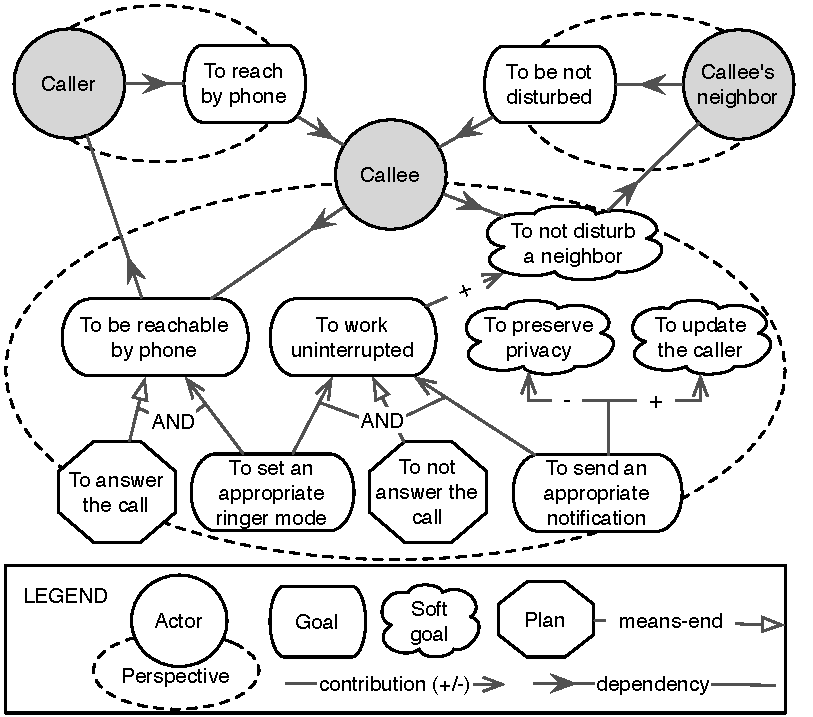
\includegraphics[angle=0,width={0.60\columnwidth}]{Chapter-3/fig/ringer-manager-tropos-actor-model.pdf}
\caption[A Tropos model of the ringer manager]{A Tropos system-as-is model of the ringer manager, expanding the callee's perspective \protect\citep{Murukannaiah-AAMAS14-Xipho}.}
\label{fig:xipho-ringer-as-is} \end{figure}

Xipho \citep{Murukannaiah-AAMAS14-Xipho} extends Tropos to engineer
personal agents. Xipho introduces \emph{context} as a high-level
abstraction and treats an actor's goals, plans, and dependencies as
inherently contextual. Xipho enables a developer to tailor a generic
model of context to a specific application scenario via systematic steps
through distinct development phases.

\subsection{Norms and Sanctions}

A norm as understood here \citep{Singh-2013-Norms} is directed from a
subject to an object and is constructed as a conditional relationship
involving an antecedent (which brings the norm in force) and a
consequent (which brings the norm to satisfaction or violation). This
representation yields clarity on who is accountable to whom. A norm can
be formalized as:
%
\begin{center}
$\N(\fsc{subject},\fsc{object}, antecedent, consequent)$
\end{center}

We employ the following types of norms in our approach. 
\begin{itemize}

\item A \emph{commitment} ($\C$) means that its subject commits to its
object to ensure the consequent if the antecedent holds. An example
commitment is that, in a meeting room, the participants may be committed
to each other to keep their phones silent: $\C$($\fsc{phone-user}$,
$\fsc{coworker}$, $\text{place}=meeting$, $\text{ring}=silent$).

\item A \emph{prohibition} means that its subject is forbidden by its
object from bringing about the consequent if the antecedent holds. An
example prohibition ($\Pro$) is that, in an examination hall, the
students may be prohibited by a proctor from answering phone calls:
$\Pro$($\fsc{phone-user}$, $\fsc{proctor}$, $\text{place}=examination$,
$\text{ring}=silent$).

\item A \emph{sanction} specifies the consequences its subject faces
from its object for satisfying or violating another norm, such as a
commitment or a prohibition. A sanction can be positive, negative, or
neutral \citep{Nardin-KER16-Classifying}. A sanction may be in the form
of ``feedback,'' e.g., a smile or a scowl, from one user to another. An
example sanction ($\San$) is that, in a meeting, if a participant's
phone rings loud, he or she receives a scowl from other meeting
participants: $\San$($\fsc{phone-user}$, $\fsc{coworker}$,
$\text{place}=meeting \land ring=loud$, $\text{feedback}=scowl$).

\end{itemize} 

\section{\frameworkA}
\label{sec:arnor-framework}

\frameworkA is a four-step method build on social constructs to systematically model the social 
experience provided by a SIPA. \frameworkA's steps include modeling of: 
\begin{enumerate*}[label=(\arabic*)]
\item goals, 
\item environmental contexts,
\item social expectations, and 
\item social experience. 
\end{enumerate*}
Figure~\ref{fig:arnor-model} shows a conceptual model of 
\frameworkA.  Table~\ref{tab:arnor-steps} provides an overview. 


\begin{figure}[!htb] 
\centering
% 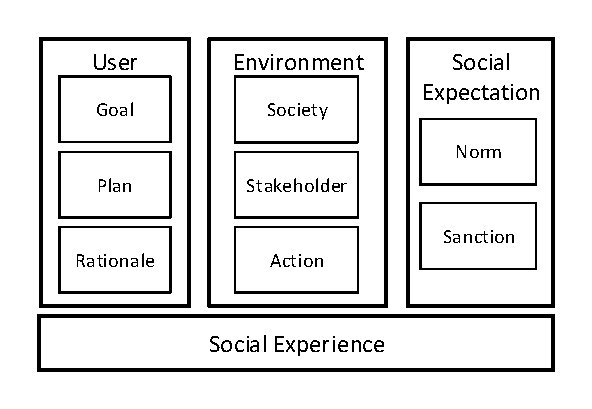
\includegraphics[angle=0,width={0.60\columnwidth}]{Chapter-3/fig/model}
\resizebox{0.6\columnwidth}{!}{

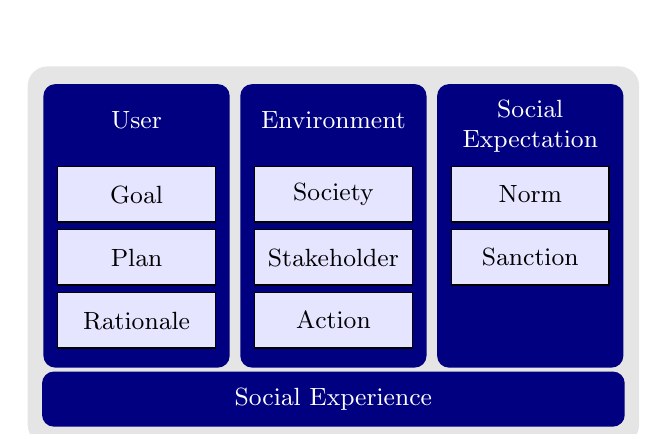
\begin{tikzpicture}[auto, node distance=2cm,>=latex',font=\small]
\tikzset{block/.style = {draw, rectangle, minimum height=2em, 
  minimum width=4em}}
\pgfdeclarelayer{background}
\pgfdeclarelayer{foreground}
\pgfsetlayers{background,main,foreground}

  \begin{pgfonlayer}{foreground}
    \node[block, fill=blue!10, minimum width = 2.0cm] (goal){Goal};
    \node[block, fill=blue!10, minimum width = 2.0cm, node distance=.8cm, below of=goal] 
      (plan){Plan};
    \node[block, fill=blue!10, minimum width = 2.0cm, node distance=.8cm, below of=plan] 
      (rationale){Rationale};


    \node[block, fill=blue!10, minimum width = 2.0cm, node distance=2.5cm, right of=goal] 
      (society){Society};
    \node[block, fill=blue!10, minimum width = 2.0cm, node distance=.8cm, below of=society] 
      (stakeholder){Stakeholder};
    \node[block, fill=blue!10, minimum width = 2.0cm, node distance=.8cm, below of=stakeholder] 
      (action){Action};
  
    \node[block, fill=blue!10, minimum width = 2.0cm, node distance=2.5cm, right of=society] 
      (norm){Norm};
    \node[block, fill=blue!10, minimum width = 2.0cm, node distance=.8cm, below of=norm] 
      (sanction){Sanction};
  
  \end{pgfonlayer}
  
  \node[fit= (goal) (plan) (rationale), inner sep=.5em, align=center, 
    minimum height = 3.6cm, minimum width = 2cm, yshift=.4cm,
    fill=blue!50!black, rounded corners=.15cm,
    label={[yshift=-.7cm, align=center, text=white]
   User}](user){};

  \node[fit= (society) (stakeholder) (action), right of=user,
    node distance=2.5cm,
    inner sep=.5em, align=center, 
    minimum height = 3.6cm, minimum width = 2cm,
    fill=blue!50!black, rounded corners=.15cm,
    label={[yshift=-.7cm, align=center, text=white]Environment}]
    (environment){};
  
  \node[fit= (norm) (sanction), right of=environment,
    node distance=2.5cm,
    inner sep=.5em, align=center, 
    minimum height = 3.6cm, minimum width = 2cm,
    fill=blue!50!black, rounded corners=.15cm,
    label={[yshift=-1.0cm, align=center, text=white]Social\\Expectation}]
    (socialexpectation){};

  \node[node distance=2.2cm, below of=environment, minimum height=.7cm,
    fill=blue!50!black, rounded corners=.15cm,
    text=white, minimum width=7.4cm] 
    (socialexperience){Social Experience};

  \begin{pgfonlayer}{background}
  \node[fit= (user) (environment) (socialexpectation)
    (socialexperience), rounded corners=.25cm, fill=gray!20,
    inner sep=.5em, align=center, minimum height = 4.8cm, minimum width = 2cm]
    (arnor){};
  \end{pgfonlayer}

\end{tikzpicture}

}
\caption[\frameworkA 's conceptual model schematically]{\frameworkA 's conceptual model schematically.}
\label{fig:arnor-model} 
\end{figure}

% Splitting table caption and heading across multiple pages: https://tex.stackexchange.com/questions/383898/how-to-split-long-table-in-multiple-pages
\clearpage
%\begin{table}[!htb]
\begin{longtable}{@{}p{2.2cm}p{5cm}p{7.5cm}@{}}
%\centering
\caption[Overview of \frameworkA tasks]{Overview of \frameworkA tasks and examples to engineer a SIPA.}
\label{tab:arnor-steps}\\
\toprule
\fbf{Step} & \fbf{\frameworkA Task} & \fbf{Example} \\\midrule

\endfirsthead
\caption[Overview of \frameworkA tasks]{Overview of \frameworkA tasks and examples to engineer a SIPA (continued).}\\
\toprule
\fbf{Step} & \fbf{\frameworkA Task} & \fbf{Example} \\\midrule

\endhead
    \midrule
    \multicolumn{3}{r}{\footnotesize\itshape Continue on the next page}
\endfoot
    \bottomrule
\endlastfoot

\multirow{1}{2.2cm}{Goal Modeling}& Identify all actors &   
Alice, Bob, Charlie, Dave, Erin, and strangers in the theater\\

& Abstract actors as primary and secondary stakeholders, as appropriate & Phone user is a primary stakeholder; friend, coworker, stranger in the vicinity of phone users are secondary stakeholders\\

& Identify goals of each actor & Phone user's goals \fsl{to be tele-reachable}, and \fsl{to be not disturbed} \\

& Identify all actions, and abstract them as appropriate &  \fsl{Phone users do not answer phone calls during meetings}; \fsl{phone users answers 
their coworkers' urgent phone calls}\\

& Identify plans for abstract actions & \fsl{Set ringer mode as loud} 
for the action \fsl{phone user answers a phone call} \\

& Associate goals with plans & Phone user's goal of \fsl{tele-reachable} 
can be realized by the plan of \fsl{setting ringer mode as loud}\\
\midrule

\multirow{1}{2.2cm}{Context Modeling} & Identify the contexts in which 
each actor's goals and plans are relevant 
	& Coworker's goal \fsl{to be not disturbed} is relevant in the \fsl{meeting} context\\
& Identify conflicting goals (and inconsistent plans) & 
Phone user's goal of \fsl{tele-reachable} conflicts with the goal \fsl{to not disturb neighbors} in the \fsl{meeting} context
\\
\midrule

\multirow{1}{2.2cm}{Social Expectation Modeling} & Identify norms relevant 
to social and privacy expectations & \fsl{The phone user is committed to
    answering urgent phone calls from family}
    \\
 & Identify possible conflicts between norms & \fsl{Phone user's commitment toward friend to answer phone calls} conflicts with
 \fsl{phone user's commitment to keep phone on silent during meeting}\\
 & Resolve conflicts by capturing contextual preferences between norms & 
   In the \fsl{meeting} context, prefer \fsl{phone user's commitment to keep phone on silent during meeting} over \fsl{phone user's commitment toward friend to answer phone calls}
   \\

\midrule
\multirow{1}{2.2cm}{Social Experience Modeling} & Identify effects of 
stakeholders' actions on social expectations & A norm that is consistently being violated, e.g., \fsl{phone users always answering calls during meeting}\\
& Promote actions that enhance social experience & 
\\

\bottomrule
\end{longtable}
%\end{table}

\subsection{Goal Modeling}

For a SIPA to provide a social experience, it needs to be aware of
the associated stakeholders, their goals and relevant plans. Goal
modeling in \frameworkA uses Tropos constructs to elicit stakeholders,
their goals, and relevant plans.

\begin{description}[leftmargin=1em]
\item[A stakeholder] is a user that participates in a society and 
interacts with or is affected by the SIPA.  \emph{Primary} stakeholders 
are the users that interact directly with the SIPA.  \emph{Secondary} 
stakeholders do not have direct interaction with the SIPA, but are 
affected by its interactions with the primary stakeholder.  

\item[A goal] is a set of states of the environment that are 
preferred by the stakeholders. 

\item[A plan] is a sequence of actions that can bring about a state in
which a stakeholder's goal is satisfied. The SIPA acts on behalf of the
stakeholders or assists stakeholders in bringing their goals.

\end{description}

Stakeholders in \frameworkA map to actors in Tropos or Xipho.
Whereas Tropos and Xipho explicitly relate actors to the users that
have goals, \frameworkA forces designers to additionally identify (secondary)
stakeholders that do not necessarily have a goal, but are affected by
the plans that (primary) stakeholders execute to achieve their
goals. Capturing secondary stakeholders is necessary to providing a 
social experience. A stakeholder may adopt different roles.

Following Table~\ref{tab:arnor-steps}, we create the goal
model for the ringer manager SIPA described in Examples~\ref{ex:ringer-meeting}--\ref{ex:ringer-accident} and Figure~\ref{fig:xipho-ringer-as-is}.

\begin{description}[leftmargin=1em]
  
  \item[Primary stakeholder.] Alice, the phone user (S$_1$). 

\item[Secondary stakeholders.] Bob (Alice's friend, S$_2$), Charlie and
Dave (Alice's coworkers, S$_3$ and S$_4$), Erin (Alice's mother, S$_5$)
and strangers (those in the theater who are in Alice's vicinity when
the ringer manager SIPA is in use, S$_6$). Here Bob, Charlie, Dave and Erin
could assume the roles of caller and neighbors in different contexts.
Note that, although the ringer manager SIPA includes only one primary
stakeholder, other settings could involve multiple primary stakeholders.

\item[Goals.] The phone user's goals are to be
tele-reachable (G$_1$), to notify caller if not reachable (G$_2$), to
work uninterrupted (G$_3$), and to avoid annoying
neighbors (G$_4$). Bob, Alice's friend has goals to (1) tele-reach Alice
(corresponds to G$_1$), and (2) be notified if Alice is not reachable
(corresponds to G$_2$). Charlie and Dave's goals are to not be disturbed
at work by anyone (same as G$_4$). Erin's mother has the same goals as
Bob. Strangers in Alice's vicinity share the same goal as Charlie and
Dave. When Charlie and Dave assume the caller role, they share Bob and 
Erin's goal of tele-reaching Alice.
  
\item[Actions.] Alice, the phone user, can answer a call if she is
available, or can notify the caller otherwise. She could
decide not to answer calls if she does not want to be disturbed or does
not want to annoy her neighbors. Based on Alice's actions, Bob, Charlie,
Dave, Erin, and other stakeholders act. For example, if Alice answers
Bob's or Erin's call, they could give Alice a positive feedback. In social
expectation modeling, we capture these feedback actions as sanctions. 

\item[Plans.] The plan corresponding to the \fsl{answer call} action is to
\fsl{set ringer mode on loud} (P$_1$). The other plans could be to
\fsl{set ringer mode on vibrate} (P$_2$) or \fsl{set ringer mode on
silent} (P$_3$).

\item[Goal-plan association.] The plan of setting the ringer on
loud promotes the phone user's goal of being tele-reachable, and
caller's goal of tele-reaching the callee. The plan of setting the
ringer on silent promotes the phone user's goal to work
uninterrupted, and the neighbors' goal of not being disturbed.
\end{description}

\subsection{Social Context Modeling}

Context modeling includes identifying social contexts in which the
stakeholders of a SIPA interact. The social context could include the
place where the interaction occurs, attributes of the place, neighbors
in the vicinity, the social relationship between primary and secondary
stakeholders, the activities the stakeholders are involved in, and so
on. The social context is decisive in identifying the goals to be
brought about or plans to be executed in case of conflicts.

Some of the contexts associated with goals, G$_1$--G$_4$, and plans,
P$_1$--P$_3$, are based on stakeholders' locations (meeting or theater),
social relationship (colleagues, friends or family), reason
associated with a phone call (urgent phone call or a casual phone
call), and so on.

Goal G$_1$ of being tele-reachable conflicts with goals
G$_3$ and G$_4$ for both the meeting and theater scenarios.
In these scenarios, the SIPA must rely on social
contexts to determine which goal to accomplish. Potentially,
where multiple plans may help realize the same goals. For example, in a
library, both the \fsl{phone on silent} plan and \fsl{phone on vibrate}
plans serve the goal of not disturbing one's neighbors. The SIPA
relies on social context to choose between multiple plans. 
%Conflicts are further handled in social expectation modeling and
%social experience modeling.
  
\subsection{Social Expectation Modeling}

Social expectations including the privacy ones influence the
stakeholders' goals and plans. We model these expectations between
stakeholders in terms of social norms and sanctions. The social norms of
a society regulate how stakeholders act and conduct themselves. Some
norms could be local to a stakeholder, for example, one's commitment
toward family members to always answer their phone calls, and some norms
could be specific to a social context, for example, in the context of a
meeting, a phone user is committed to keep his or her phone silent.

We express social expectations for the ringer manager SIPA via norms,
sanctions and conflicts.
\begin{description}[leftmargin=1em]
\item[Norms.] We identify the following norms.
  \begin{itemize}[leftmargin=1em]
  \item A phone user is committed to answering phone calls from
  callers. This commitment is satisfied by the plan of setting the 
  ringer mode on loud.

  $C_{caller}$: $\C(\fsc{phone-user},\fsc{caller}, \text{call}, \text{ring}=\textit{loud})$

  \item A phone user is committed to notifying the caller if he or she does
  not answer. The commitment is satisfied by the plan of setting the
  ringer mode on silent and sending a notification to the caller.
  
  $C_{notify}$: $\C(\fsc{phone-user},\fsc{caller}, \text{call},\\ 
  \text{ring}= \textit{silent}   \land \textit{notify})$
    
  \item A phone user is committed to coworkers to not let the phone ring 
  during meetings.
  This commitment is satisfied by the plan of setting the ringer mode on 
  silent or vibrate. 

  $C_{meeting}$: $\C(\fsc{phone-user},\fsc{coworkers}, \text{call},\\ 
  \text{ring}= \textit{silent} \lor \text{ring} = \textit{vibrate})$
  \end{itemize}
  
\item[Sanctions.] The associated sanctions are as below: 
  \begin{itemize}[leftmargin=1em]
  \item A phone user is (negatively) sanctioned by coworkers for 
  answering a phone call during a meeting. 
  
    $S_{meeting}$: $\C(\fsc{phone-user},\fsc{coworkers}, \text{call} \\
    \land \text{place}=\textit{meeting} \land \text{ring}=\textit{loud}, \text{feedback}=\textit{negative})$
  \end{itemize}
  
  \item[Conflicts.] If a caller calls the phone user during a meeting, the phone 
  user's commitment $C_{caller}$ toward a caller conflicts with his or her 
  commitment $C_{meeting}$ toward coworkers to not answer phone calls 
  during meetings, i.e., \\$\mathit{conflict}(C_{caller}, C_{meeting})$.
    
\end{description}

Conflicts in social expectations can be resolved by capturing contextual 
preferences between conflicting norms. For example, a phone user can have a 
preference of  $C_{meeting}$ (\fsl{keep phone on silent during meetings})
to $C_{caller}$ (\fsl{answer calls from family members}). 

\subsection{Social Experience Modeling}
Norms are satisfied or violated as stakeholders act and execute plans to
achieve their goals. Norm satisfaction or violation provides positive or
negative experience to the stakeholders. As agents derive social
experience from norms, over time, certain norms are preferred over
others, and some lose significance. If a certain phone user is always
answering phone calls during meetings, the phone user could be banished
from meetings. A SIPA should execute actions that promote yield social
experience by choosing which plans to execute, which goal states to
accomplish, and which norms to satisfy. To decide which actions to
promote, SIPAs could employ argumentation
\citep{BenchCapon-2007-Argumentation+AI}, and make use of argumentation
schemes such as \emph{arguments from consequences}, and \emph{arguments
from popular opinion} \citep{walton2008argumentation}. Additionally, a
SIPA, depending upon its user's privacy attitude and information sharing
preferences, can choose to share its decision rationale for choosing an
action with the other stakeholders. The sharing of rationale could
introduce nuances in social relationships of a SIPA's stakeholders such
as increase of trust that we do not model.



\section{Evaluation}
\label{sec:arnor-experiments}

We investigate our research question by evaluating \frameworkA via a
developer study and a simulation experiment.


\subsection{Developer Study}
\label{sec:devstudy}

We begin with a multiphase developer study in
which participants develop ringer manager SIPAs. Our study was approved
by the Institutional Review Board (IRB). We obtained informed consent
from each participant. The developer study lasted for six weeks.

\begin{figure}[!htb] \centering
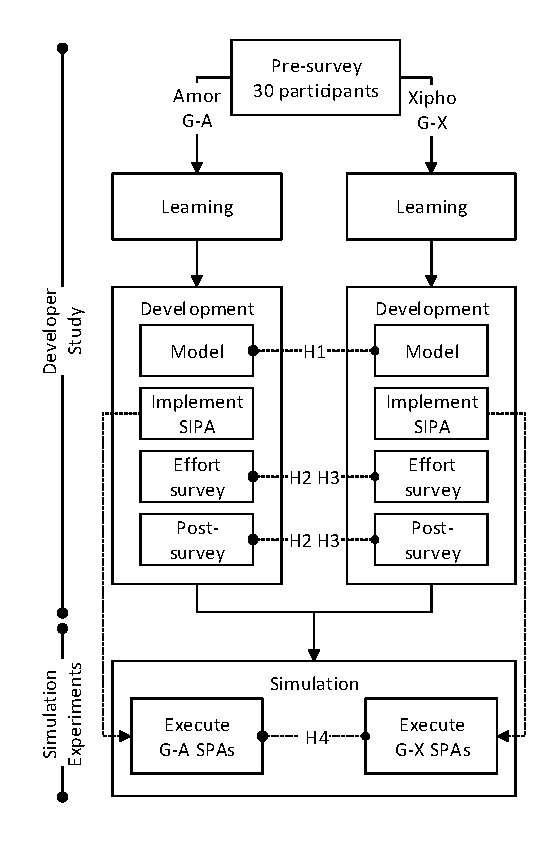
\includegraphics[angle=0,width={0.60\columnwidth}]{Chapter-3/fig/design}
\caption[Experimental design]{Experimental design.}
\label{fig:design} \end{figure}

\subsubsection*{Study Unit} 

The study unit is a ringer manager SIPA discussed 
in Examples~\ref{ex:ringer-meeting}--\ref{ex:ringer-accident} and Figure~\ref{fig:xipho-ringer-as-is}.

\subsubsection*{Participants}

The developer study involved 30 participants, enrolled in a
graduate-level computer science course. The participants earned points
toward their course grades for completing the tasks described. However,
participation in the study was not mandatory. Nonparticipants were
offered an alternative task to earn points equivalent to what they would
earn by participating in the study.

\subsubsection*{Study Mechanics}

This developer study has two phases: learning and development.  The study 
follows the one-factor design with two alternatives (\frameworkA and Xipho).  
We use Xipho as our baseline method because it is best suited among the
existing AOSE methods to engineer personal agents.

We split participants into two groups (A that follows \frameworkA, and X
that follows Xipho) balanced on skills indicated in a presurvey
(detailed in Appendix~\ref{appsec:presurvey}). All participants develop
a ringer manager SIPA.

\begin{description}[leftmargin=1em]

\item[Learning Phase.] During the learning phase of the study,
participants proposed a SIPA, and created models of the proposed SIPA.
This phase sought to help participants understand the nuances of a SIPA,
and to teach them how to model requirements. The data collected in the
learning phase is not used in the evaluation. 

\item[Development Phase.] In the development phase, participants
modeled and implemented a ringer manager SIPA that adapts according
to expectations of callers and 
neighbors, and sanctions received from callers and
neighbors for each action.

\end{description}

In the two development phases, participants were provided with a testbed
to verify the working of their SIPAs.

\subsubsection*{Deliverables}

The participants submitted models and source code at the completion of
the development phase. Additionally, the participants completed a time
and effort survey (detailed in Appendix~\ref{appsec:effortsurvey}) for
each work session, and completed a post-phase survey (detailed in
Appendix~\ref{appsec:postsurvey}) at the end of each phase.

\subsubsection*{Metrics}

To measure the effectiveness of \frameworkA, we compute the following metrics.

\begin{description}[leftmargin=1em]
\item[Model coverage] measures the completeness of the model. It is the
ratio of the number of requirements identified correctly in the produced
model to the total number of requirements of the SIPA. Higher is better.

\item[Model correctness] measures how correct the model is.  It is the
ratio of the number of correctly identified requirements to the total
number of requirements of the SIPA identified.  Higher is better.

\item[Model quality] is the product of model coverage and model
correctness. Higher is better.

\item[Time to develop] is the actual time spent by participants in hours
to develop the SIPA.  Lower is better.

\item[Difficulty of development] is the subjective rating by
participants on how easy it is to develop the SIPA on a Likert scale of
1 (very easy) to 7 (very difficult). Lower is better.

\item[Effort to develop] is the product of time spent in hours and ease
of development rating for each work session. Lower is better.
\end{description}

\subsubsection*{Hypotheses}

We consider the following hypotheses.

\bhypothesis

\item Developers who follow \frameworkA produce better quality models 
than those who follow Xipho.  

\item Developers who follow \frameworkA spend less time to develop 
a SIPA, than those who follow Xipho.

\item Developers who follow \frameworkA feel it is easier to develop 
a SIPA, than those who follow Xipho.

\item Developers who follow \frameworkA expend less effort to develop 
a SIPA, than those who follow Xipho.

\ehypothesis

\subsubsection*{Threats and Mitigation}

We mitigated three main threats to our studies. Differences amongst
participants' programming and modeling skills are inevitable. To handle
the skill differences between participants, we surveyed participants
about their educational backgrounds and prior experiences with
programming and conceptual modeling. We balanced the two groups based on
the survey. To mitigate the risk of participants' failing to report information,
participants were instructed to complete a time and effort survey after
each work session, while it was fresh in their minds. Communication
between participants of different groups is yet another threat. To
mitigate the risk of contamination, we created separate message boards for each
participant group, and restricted participants to only posting
clarification questions on the group message boards.



\subsection{Simulation Experiments}
\label{sec:arnor-simulation}

We further investigate our research question via simulation experiments.
We execute the ringer manager SIPAs implemented by third-party
developers (as part of the aforementioned developer study) on a testbed
fabricated to simulate different real-world environments.


\subsubsection*{Ringer adaptation scenarios}

To test runtime adaptability, we test the applications for
multiple iterations of incoming phone calls during a meeting.

\begin{description}[leftmargin=1em]
\item[Norms fixed.] 
The meeting room participants are committed to keeping their 
phones silent.

\item[Change in norms.] 
The meeting room participants are initially committed to keeping their
phones silent, but later the commitment expires. 

\item[Change in context.] 
The meeting room participants are always committed to keeping their
phones silent. Initially there are several participants in the meeting, but later
all but two leave the meeting.

\item[Change in sanction.] 
The meeting room participants are always committed to keeping their 
phones silent. Initially they give negative feedbacks for loud ringing
but later give more neutral feedbacks. 
\end{description}


\subsubsection*{Metrics}

To measure social experience, we compute the following social metrics
in each of the above adaptation scenarios. 
\begin{description}[leftmargin=1em] 
\item[Adaptability coverage] measures the completeness of code for
adaptability requirements. It is the ratio of the number of adaptability
requirements implemented correctly to the total number of adaptability
requirements. Higher is better.

\item[Adaptability correctness] measures the correctness of the code for
adaptability requirements. It is the ratio of the number of correctly 
implemented adaptability requirements to the total number of adaptability
requirements implemented. Higher is better.

\item[Norm compliance] refers to the proportion of norm instances that
are satisfied. Higher is better.

\item[Sanction proportion] measures the percentage of sanctions imposed.
Lower is better.
\end{description}

\subsubsection*{Hypotheses}

We consider these additional hypotheses:

\bhypothesis

\item SIPAs developed using \frameworkA yields better adaptability
than SIPAs developed using Xipho.

\item SIPAs developed using \frameworkA provide a richer social
experience than SIPAs developed using Xipho.

\ehypothesis

We use adaptability coverage and correctness to test hypothesis
H$_5$, and use norm compliance and sanction proportion measures to test
hypothesis H$_6$.

\section{Results}
\label{sec:arnor-result}

We analyze deliverables produced by participants at the end of each
phase, and compute the study parameters for each deliverable.  

\subsection{Developer Study}

To test hypothesis H$_1$, we compare the models produced by Groups A and X.
For hypothesis H$_2$, we compare the development time expended by
Groups A and X during the two development phases. For
hypothesis H$_3$, we compare the ease of development ratings reported by
Groups A and X during the two development phases, and
for hypothesis H$_4$, we compare their expended effort.

\begin{description}[leftmargin=1em]
\item[Model quality.] We evaluated models produced by the participants 
for correctness and coverage, and computed a quality metric.  We found 
no significant difference in model quality. 

\item[Time and effort to develop.] We found that average time ($13.27$
hours) and effort ($61.54$) expended by the participants using
\frameworkA to be lower than average time ($17.72$ hours) and effort
($96.6$) expended by the participants using Xipho.
Figures~\ref{fig:dev-time} and \ref{fig:dev-effort} show the boxplots
for time and effort expended by participants using \frameworkA and Xipho
to develop the social ringer SIPA.

\begin{figure}[!htb] \centering
  \begin{tikzpicture}
    \tikzstyle{every node}=[font=\small]
    \begin{axis}[
	y=0.7cm,
	ytick={1,2,3,4},
	yticklabel style={align=center},
	yticklabels={Xipho,\frameworkA},
	width=10cm,
	xtick={1,5,10,15,20,25},
	xlabel={Time in hours},
	xlabel style={align=center},
	xmin=0, xmax=30,
	boxplot/average=auto,
	title style={align=center},
	title={Development Time},
	title style={yshift=-1ex,},
	]
	\addplot+[red,boxplot,mark options={fill=red}]
	table[x expr=\coordindex, y index=0]
	{Chapter-3/data/X-dev-time.csv};
	\addplot+[blue,boxplot,mark options={fill=blue}]
	table[x expr=\coordindex, y index=0]
	{Chapter-3/data/A-dev-time.csv};

    \end{axis}
  \end{tikzpicture}
\caption[\frameworkA vs.\ Xipho: Development time]{\frameworkA vs.\ Xipho's development time in hours as reported 
in the work session surveys.}
\label{fig:dev-time}
\end{figure}

\item[Difficulty of development.] The participants using \frameworkA 
found it easier to develop SIPAs with \frameworkA, compared to
participants using Xipho. Figure~\ref{fig:dev-ease} shows the difficulty of
development boxplots.


\begin{figure}[!htb] \centering
  \begin{tikzpicture}
    \tikzstyle{every node}=[font=\small]
    \begin{axis}[
	y=0.7cm,
	ytick={1,2,3,4},
	yticklabel style={align=center},
	yticklabels={Xipho,\frameworkA},
	width=10cm,
	xtick={10,50,100,150},
	xlabel={Effort},
	xmin=0, xmax=160,
	xlabel style={align=center},
	boxplot/average=auto,
	title style={align=center},
	title={Development Effort},
	title style={yshift=-1ex,},
	]
	\addplot+[red,boxplot,mark options={fill=red}]
	table[x expr=\coordindex, y index=0]
	{Chapter-3/data/X-dev-effort.csv};
	\addplot+[blue,boxplot,mark options={fill=blue}]
	table[x expr=\coordindex, y index=0]
	{Chapter-3/data/A-dev-effort.csv};

    \end{axis}
  \end{tikzpicture}
\caption[\frameworkA vs.\ Xipho: Development effort]{\frameworkA vs.\ Xipho's development effort as reported in the work 
session surveys.}
\label{fig:dev-effort}
\end{figure}

\begin{figure}[!htb] \centering
  \begin{tikzpicture}
    \tikzstyle{every node}=[font=\small]
    \begin{axis}[
	y=0.7cm,
	ytick={1,2,3,4},
	yticklabel style={align=center},
	yticklabels={Xipho,\frameworkA},
	width=10cm,
	xtick={1,2,3,4,5,6,7},
	xlabel={},
	xlabel style={align=center},
	xmin=1, xmax=7,
	boxplot/average=auto,
	title style={align=center},
	title={Model},
	title style={yshift=-1ex,},
	]
	\addplot+[red,boxplot,mark options={fill=red}]
	table[x expr=\coordindex, y index=0,col sep=comma]
	{Chapter-3/data/X-dev-ease.csv};
	\addplot+[blue,boxplot,mark options={fill=blue}]
	table[x expr=\coordindex, y index=0,col sep=comma]
	{Chapter-3/data/A-dev-ease.csv};

    \end{axis}
  \end{tikzpicture}

  \vspace{2em}
%

  \begin{tikzpicture}
    \tikzstyle{every node}=[font=\small]
    \begin{axis}[
	y=0.7cm,
	ytick={1,2,3,4},
	yticklabels={Xipho,\frameworkA},
	width=10cm,
	xtick={1,2,3,4,5,6,7},
	xlabel={},
	xlabel style={align=center},
	xmin=1, xmax=7,
	boxplot/average=auto,
	title style={align=center},
	title={Implementation},
	title style={yshift=-1ex,},
	]
	\addplot+[red,boxplot,mark options={fill=red}]
	table[x expr=\coordindex, y index=1,col sep=comma]
	{Chapter-3/data/X-dev-ease.csv};
	\addplot+[blue,boxplot,mark options={fill=blue}]
	table[x expr=\coordindex, y index=1,col sep=comma]
	{Chapter-3/data/A-dev-ease.csv};

    \end{axis}
  \end{tikzpicture}

  \vspace{2em}
%

  \begin{tikzpicture}
    \tikzstyle{every node}=[font=\small]
    \begin{axis}[
	y=0.7cm,
	ytick={1,2,3,4},
	yticklabels={Xipho,\frameworkA},
	width=10cm,
	xtick={1,2,3,4,5,6,7},
	xlabel={},
	xlabel style={align=center},
	xmin=1, xmax=7,
	boxplot/average=auto,
	title style={align=center},
	title={Testing},
	title style={yshift=-1ex,},
	]
	\addplot+[red,boxplot,mark options={fill=red}]
	table[x expr=\coordindex, y index=2,col sep=comma]
	{Chapter-3/data/X-dev-ease.csv};
	\addplot+[blue,boxplot,mark options={fill=blue}]
	table[x expr=\coordindex, y index=2,col sep=comma]
	{Chapter-3/data/A-dev-ease.csv};

    \end{axis}
  \end{tikzpicture}

\caption[\frameworkA vs.\ Xipho: Difficulty of development]{\frameworkA vs.\ Xipho's difficulty of development on a Likert scale of 1 (very easy) to 7 (very difficult).}
\label{fig:dev-ease}
\end{figure}

\end{description}

\subsection{Simulation Experiments}

To evaluate H$_5$ and H$_6$, we analyzed the SIPA's implementation code
and executed the SIPAs in diverse scenarios. We compare the execution
results of \frameworkA and Xipho groups.

\begin{description}[leftmargin=1em]

\item[Adaptability features.] We found average adaptability coverage
($80$\%) to be the same for SIPAs developed by the \frameworkA and Xipho
groups. This result could be attributed to the limited time we gave the
participants to develop the SIPA. Average adaptability correctness was
found to be higher for \frameworkA ($100$\%) compared to the Xipho
($95$\%). This gain could be attributed to the systematic steps provided
by \frameworkA to engineer SIPAs.

\item[Norm compliance.]  Figure~\ref{fig:simulation-compliance} shows 
line plots for norm compliance in the four ringer adaptation scenarios. Though 
the average norm compliance values for SIPAs developed using \frameworkA and Xipho 
are mostly similar, \frameworkA performs slightly better in the fixed norms scenario. 

\begin{figure}[!tb]
    \centering
    \begin{tikzpicture}
    \begin{axis}[
        title={Norms fixed},
        height=7cm,
        width=7cm,
        xlabel={Time tick},
        ylabel={Norm Compliance \%},
        xmin=1, xmax=10,
        ymin=0, ymax=100,
        xtick={1,2,3,4,5,6,7,8,9,10},
        legend pos=north west,
        legend style={font=\small},
        ymajorgrids=true,
        grid style=dashed,
        ]

        \addplot table [x=tick, y=percentage, col sep=comma] {Chapter-3/data/A-compliance-1.csv};
        \addplot table [x=tick, y=percentage, col sep=comma] {Chapter-3/data/X-compliance-1.csv};
        \legend{\frameworkA,Xipho}

    \end{axis}
  
    \end{tikzpicture}
    \hspace{2em}
    \begin{tikzpicture}
    \begin{axis}[
        title={Change in norms},
        height=7cm,
        width=7cm,
        xlabel={Time tick},
        %ylabel={Norm Compliance \%},
        xmin=1, xmax=10,
        ymin=0, ymax=100,
        xtick={1,2,3,4,5,6,7,8,9,10},
        yticklabel=\empty,
        legend pos=north west,
        legend style={font=\small},
        ymajorgrids=true,
        grid style=dashed,
        ]

        \addplot table [x=tick, y=percentage, col sep=comma] {Chapter-3/data/A-compliance-2.csv};
        \addplot table [x=tick, y=percentage, col sep=comma] {Chapter-3/data/X-compliance-2.csv};
        \addplot +[mark=none,dashed] coordinates {(5, 0) (5, 100)};
        \legend{\frameworkA,Xipho}

    \end{axis}
    
    \end{tikzpicture}
    
    \vspace{2em}

    \begin{tikzpicture}
    \begin{axis}[
        title={Change in context},
        height=7cm,
        width=7cm,
        xlabel={Time tick},
        ylabel={Norm Compliance \%},
        xmin=1, xmax=10,
        ymin=0, ymax=100,
        xtick={1,2,3,4,5,6,7,8,9,10},
        legend pos=north west,
        legend style={font=\small},
        ymajorgrids=true,
        grid style=dashed,
        ]

        \addplot table [x=tick, y=percentage, col sep=comma] {Chapter-3/data/A-compliance-3.csv};
        \addplot table [x=tick, y=percentage, col sep=comma] {Chapter-3/data/X-compliance-3.csv};
        \addplot +[mark=none,dashed] coordinates {(5, 0) (5, 100)};
        \legend{\frameworkA,Xipho}

    \end{axis}
    
    \end{tikzpicture}
    \hspace{2em}
    \begin{tikzpicture}
    \begin{axis}[
        title={Change in sanction},
        height=7cm,
        width=7cm,
        xlabel={Time tick},
        %ylabel={Norm Compliance \%},
        xmin=1, xmax=10,
        ymin=0, ymax=100,
        xtick={1,2,3,4,5,6,7,8,9,10},
        yticklabel=\empty,
        legend pos=north west,
        legend style={font=\small},
        ymajorgrids=true,
        grid style=dashed,
        ]

        \addplot table [x=tick, y=percentage, col sep=comma] {Chapter-3/data/A-compliance-4.csv};
        \addplot table [x=tick, y=percentage, col sep=comma] {Chapter-3/data/X-compliance-4.csv};
        \addplot +[mark=none,dashed] coordinates {(5, 0) (5, 100)};
        \legend{\frameworkA,Xipho}

    \end{axis}
    
    \end{tikzpicture}
    \caption[\frameworkA vs.\ Xipho: Norm compliance]{\frameworkA vs.\ Xipho's norm compliance.}
    \label{fig:simulation-compliance}
\end{figure}

\item[Sanction proportion.] Figure~\ref{fig:simulation-sanction-count}
shows the plots for sanction proportion in the four adaptation scenarios.
For the first three scenarios (norms fixed, norms change, and
context change), the SIPAs developed using \frameworkA have a lower
sanction proportion. For the sanction change adaptation scenario, the SIPAs
developed using \frameworkA take slightly longer to adapt, and only have
a slightly higher sanction proportion than the SIPAs developed using Xipho.

\begin{figure}[!tb]
    \centering
    \begin{tikzpicture}
    \begin{axis}[
        title={Norms fixed},
        height=7cm,
        width=7cm,
        xlabel={Time tick},
        ylabel={Sanction \%},
        xmin=1, xmax=10,
        ymin=0, ymax=100,
        xtick={1,2,3,4,5,6,7,8,9,10},
        legend pos=south west,
        legend style={font=\small},
        ymajorgrids=true,
        grid style=dashed,
        ]

        \addplot table [x=tick, y=percentage, col sep=comma] {Chapter-3/data/A-sanction-1.csv};
        \addplot table [x=tick, y=percentage, col sep=comma] {Chapter-3/data/X-sanction-1.csv};
        \legend{\frameworkA,Xipho}

    \end{axis}
    
    \end{tikzpicture}
  \hspace{2em}
    \begin{tikzpicture}
    \begin{axis}[
        title={Change in norms},
        height=7cm,
        width=7cm,
        xlabel={Time tick},
        xmin=1, xmax=10,
        ymin=0, ymax=100,
        xtick={1,2,3,4,5,6,7,8,9,10},
        yticklabel=\empty,
        legend pos=south west,
        legend style={font=\small},
        ymajorgrids=true,
        grid style=dashed,
        ]

        \addplot table [x=tick, y=percentage, col sep=comma] {Chapter-3/data/A-sanction-2.csv};
        \addplot table [x=tick, y=percentage, col sep=comma] {Chapter-3/data/X-sanction-2.csv};
        \addplot +[mark=none,dashed] coordinates {(5, 0) (5, 100)};
        \legend{\frameworkA,Xipho}

    \end{axis}
    
    \end{tikzpicture}

    \vspace{2em}

    \begin{tikzpicture}
    \begin{axis}[
        title={Change in context},
        height=7cm,
        width=7cm,
        xlabel={Time tick},
        ylabel={Sanction \%},
        xmin=1, xmax=10,
        ymin=0, ymax=100,
        xtick={1,2,3,4,5,6,7,8,9,10},
        legend pos=south west,
        legend style={font=\small},
        ymajorgrids=true,
        grid style=dashed,
        ]

        \addplot table [x=tick, y=percentage, col sep=comma] {Chapter-3/data/A-sanction-3.csv};
        \addplot table [x=tick, y=percentage, col sep=comma] {Chapter-3/data/X-sanction-3.csv};
        \addplot +[mark=none,dashed] coordinates {(5, 0) (5, 100)};
        \legend{\frameworkA,Xipho}

    \end{axis}
    
    \end{tikzpicture}
  \hspace{2em}
    \begin{tikzpicture}
    \begin{axis}[
        title={Change in sanction},
        height=7cm,
        width=7cm,
        xlabel={Time tick},
        xmin=1, xmax=10,
        ymin=0, ymax=100,
        xtick={1,2,3,4,5,6,7,8,9,10},
        yticklabel=\empty,
        legend pos=south west,
        legend style={font=\small},
        ymajorgrids=true,
        grid style=dashed,
        ]

        \addplot table [x=tick, y=percentage, col sep=comma] {Chapter-3/data/A-sanction-4.csv};
        \addplot table [x=tick, y=percentage, col sep=comma] {Chapter-3/data/X-sanction-4.csv};
        \addplot +[mark=none,dashed] coordinates {(5, 0) (5, 100)};
        \legend{\frameworkA,Xipho}

    \end{axis}
    \end{tikzpicture}
    \caption[\frameworkA vs.\ Xipho: Sanction proportion]{\frameworkA vs.\ Xipho's sanction proportion.}
    \label{fig:simulation-sanction-count}
\end{figure}

\end{description}

\subsection{Threats to Validity}
\label{sec:threats-to-validity}

In the developer study, we mitigated the threats of skills difference,
participants' failure to report information, and the risk of
contamination. However, some threats remain.

First, our results are based only on the development of a single SIPA
(ringer). For conclusive results on the effectiveness of \frameworkA,
future studies may require participants to develop more than one kind of
SIPA.

Second, the SIPAs developed by the study participants mostly reflect the
participants' (developers) privacy attitudes and information sharing
preferences. To generalize our results, it is required to collect real
data on SIPA users' privacy attitudes and information sharing
preferences.

Third, in simulation experiments, we tested runtime adaptability of
SIPAs under diverse, but a limited set of scenarios. The scenarios we
incorporated may not represent all real world scenarios in which a
ringer SIPA would be employed.

Collecting real data about users' attitudes, preferences, and contexts
is essential, though nontrivial, to mitigate the second and third
threat. Crowdsourcing is a promising avenue for future studies to
collect such data at a large scale.

\section{Related Works}
\label{sec:arnor-related}

\citet{Ali-2013-Reasoning} propose an AOSE-based contextual 
requirements engineering framework, with a focus on consistency and
conflict analysis.  \frameworkA goes beyond conflict analysis, and 
promotes goals, plans, and norms that promote greater social experience. 
\citet{Rahwan-2006-Integrating} propose a framework
to integrate goal models and social models. \frameworkA models subsume
social models, and provide richer abstractions to capture agents'
interactions and affects on experience. 

\citet{Sugawara-IJCAI11-Emergence} attempt to resolve
conflicts through reinforcement learning. \citet{Mashayekhi-IJCAI16-Silk} propose a hybrid mechanism to monitor
interactions and recommend norms to resolve conflicts. 
\citet{Mihaylov-2014-Decentralized} study convergence and propose a
decentralized approach based on strategies in game theory. 
\citet{Villatoro-TAAS13-Robust} introduce social instruments to
facilitate norm emergence via social learning. 
\citet{Yu-AAMAS13-Emergence} study norm emergence through collective
learning from local interactions, and find that collective learning is
superior to pairwise learning. \frameworkA provides constructs to
engineer socially adaptable SIPAs that can make use of these approaches
for norm emergence.

\citet{Hao-FSE16-Norms+formal} propose a lightweight formal
method to design normative systems, which uses Alloy modeling language
and analyzer to synthesize and refine norms. 
\Citet{vanRiemsdijk-AAMAS15-SociallyAdaptive} propose a semantic norm
compliance framework for socially adaptive agents. They use LTL to
express norms. Agents in van Riemsdijk {\etal}'s framework identify and
adopt new norms, and determine execution mechanisms to comply to these
norms. \citet{Aldewereld-TAAS16-GroupNorms} present a
formalism for group norms, and provide mechanisms to reason about these
norms. \citet{Ajmeri-IJCAI16-Coco} propose Coco, a
formalism to express and reason about conflicting commitment instances
at runtime, and dominance among them. Coco employs Answer Set
Programming to compute the nondominated commitment instances and
determines compliance of actions with nondominated commitment instances.
These formalisms could use \frameworkA's social constructs to assist
SIPAs in compliance, adoption of new norm, and resolution of conflicts
amongst norms at runtime.

\section{Conclusion and Future Directions}
\label{sec:arnor-discussion}

We advance the science of privacy by tackling nuanced notions of
privacy, including intrusion, disapprobation, and information leakage,
in personal agents. We treat respecting stakeholders' privacy as an
inherent aspect of delivering a social experience. We envision socially
intelligent personal agents that
\begin{enumerate*}[label=(\arabic*)]
\item adapt to the social contexts of their stakeholders; and
\item act and interact in their best interest (not just the primary stakeholder).  
\end{enumerate*}

We develop \frameworkA, a method that provides social constructs to
engineer privacy-aware social agents. We demonstrate the method via a
ringer manager SIPA. We evaluate \frameworkA using a developer study and
simulation experiments. Compared to Xipho, we find that \frameworkA
\begin{enumerate*}[label=(\arabic*)]
\item facilitates faster development of SIPAs; and
\item yields SIPAs of higher quality, higher adaptability correctness, 
lower sanction proportion, and similar adaptability coverage and norm compliance.
\end{enumerate*}
These observations suggest that \frameworkA promotes SIPAs to deliver a rich 
social experience.

\subsection*{Future Directions}

\citet{Ferreira-AAAI13-GroupRelations} propose a
computational model for emotional agents that considers norms, social
relations, roles and socially acceptable behaviors in a given context.
\citet{Sollenberger-AAMAS11-Kokomo} introduce Kokomo 
to develop affective applications, and provide a middleware for building 
such applications. 
Incorporating an affective \citep{Sollenberger-AAMAS11-Kokomo} and emotional
basis of norms in social agents is an interesting future direction.
Modeling affect could assist SIPAs learn contextually relevant norms. 
A middleware implementation of \frameworkA could facilitate development.

\citet{TOCHI-17:Multiuser} study how context, users' preferences, 
and arguments influence a sharing decision in a multiuser privacy scenario. 
They collect data about appropriate sharing policies for a variety of multiuser
scenarios from human participants in a large scale study. We conjecture that 
such data can be used to seed SIPAs with an initial set of norms, which the 
SIPAs can evolve once put to use.

%------------------------------%
\chapter[Understanding Social Context]{Understanding and Reasoning about Social Context}
\label{chap:poros}
%------------------------------%

This chapter describes \frameworkB, our approach for building
personal agents that carry out enriched interactions where deviating
agents share selected elements of their contexts, and others
respond appropriately, and its empirical evaluation via 
simulation experiments. It is based on a paper ``Robust Norm 
Emergence by Revealing and Reasoning about Context: Socially 
Intelligent Agents for Enhancing Privacy'' that appears in 
\emph{ Proceedings of the 27th International Joint Conference 
on Artificial Intelligence (IJCAI)}.

\section{Introduction}
\label{sec:Poros-intro}

Social \emph{norms} provide a robust means to regulate interactions in 
human society. Our everyday actions tend to \emph{comply} with social norms. For example, \fsl{ignoring a phone call during a 
meeting} and \fsl{remaining silent in a public library} are expected 
behaviors that accord with social norms. However,  we often \emph{deviate} from the applicable social norms, for 
instance, when \fsl{stepping out of a meeting to answer a phone call}.

The ability to deviate from norms is crucial for autonomy. We 
may \emph{sanction} each other based on how we
are interacting. In particular, negative sanctions in response to
deviations are a means for establishing norms \citep{Andrighetto-2013-PunishVoice}. 
For example, when a meeting attendee's phone rings, a \fsl{scowl} on other attendees'
faces hints at a norm of \fsl{keeping one's phone silent
during meetings}.

Existing approaches for norms provide simplified interactions: a deviation or not, followed by a sanction or not. But real-life interactions are more complex. Whether a deviation leads to a positive or negative sanction depends on 
how others perceive its \emph{context} or circumstances of occurrence. 
When we deviate from a norm, we may offer an apology, describing the 
context. One, revealing context may soften a deviation and help avert 
negative sanctions. Suppose, upon receiving a call during a meeting, 
Alice says that the call was from her sick father. As a result, the meeting attendees may excuse Alice for taking 
the call. A deviation may result in a positive sanction. For instance, 
a physician who reveals a patient's private data to save the patient's life 
would receive a positive sanction despite violating a norm. 
Even in the phone call setting, a positive sanction may ensue for deviating from a norm. For
example, a user who hesitantly takes a call from his nine-month
pregnant wife during a lab meeting would generally receive positive
comments from coworkers.
%
Two, context helps refine the relevant norms. For example, Alice's 
revelation may help refine the norm from \fsl{ignoring a phone call 
during a meeting} to \fsl{ignoring a phone call during a meeting, unless 
the call is urgent}. In essence, deviation context and any ensuing 
sanction help characterize the boundaries of a norm in play.

Accordingly, we propose \frameworkB, an approach for building agents that carry out enriched interactions where deviating agents share selected elements of their contexts, and others respond appropriately. A socially intelligent personal agent (SIPA) is an agent who acts in accordance with (but may deviate from) social norms \citep{Ajmeri-AAMAS17-Arnor}.  
%
We imagine an artificial agent society in which SIPAs of three main types act and interact on behalf of (human) users, as a basis for empirically investigating the emergence and quality of norms. 

This research applies in developing privacy-supporting SIPAs. Norms provide a basis for understanding privacy \citep{Nissenbaum-11:online}. Regulations about information disclosure, as in healthcare, are context-dependent norms \citep{Ajmeri-IJCAI16-Coco}, as are social practices. Privacy involves control over when and what information to disclose \citep{westin1967privacy}. In some construals, actions that intrude upon one's solitude or bring disapprobation are privacy violations. In essence, all privacy-relevant interactions are modulated by norms.  Therefore, social intelligence in making decisions cognizant of norms while preserving social cohesion is crucial.

%\paragraph{Contribution}
%
Our main contribution is to study two research questions in light of a specific decision by a SIPA, namely, whether to reveal its context to others when it deviates from a norm:

\begin{description}
\item[Q$_1$ Norm:] Does revealing context and reasoning about revealed context promote emergence of robust social norms? 
\item[Q$_2$ Goal:] Does acting in accordance to such robust norms result in an improved goal satisfaction?
\end{description}

Our results show that (1) norms that emerge in \frameworkB are robust, implying improved social cohesion and (2) SIPAs yield higher goal satisfaction to their users when acting in \frameworkB than when acting in a conventional setting (just sanctions). 

\section{Related Work}
\label{sec:Poros-related-work}

Research on normative systems has addressed the problems of conflict, 
compliance, and emergence of norms. We sample some of the literature from the following themes.

%\paragraph{Social Norms and Multiagent Systems}
\emph{Social norms} regulate agent interactions by characterizing
what behavior one agent may legitimately expect from another in a particular 
setting \citep{Kafali-IS16-Revani,Singh-2013-Norms}. 
%
We adopt Singh's \shortcite{Singh-2013-Norms} computational representation 
of social norms. A norm is directed from a subject (stakeholder) to an 
object (stakeholder), and is constructed
as a conditional relationship involving an antecedent (which brings the
norm into force) and a consequent (which brings the norm to satisfaction
or violation). 
Ajmeri {\etal} \shortcite{Ajmeri-AAMAS17-Arnor} 
introduce Arnor, a method to model social intelligence in personal agents. 
They argue that personal agents who understand 
the intricacies of social norms, deviations, and associated arguments can 
provide a privacy-preserving social experience to their users. 

%\paragraph{Context Sharing}
Works on designing \emph{context-aware} agents emphasize modeling \citep{Murukannaiah-AAMAS14-Xipho} and sharing \citep{Ajmeri-AAMAS17-Arnor}. 
\frameworkB is novel in the way it helps SIPAs infer social norms by 
revealing deviation context and reasoning about context revealed by others. \frameworkB
examines the effect of revealing context by agents after norm
deviations. K{\"o}kciyan and Yolum \shortcite{Kokciyan-IJCAI17-Privacy} 
propose an argumentation-based approach to enable agents to reason about context and reveal information based on it. Whereas their focus is on understanding the context to make a privacy decision, we demonstrate the benefits of revealing context. 
%
Naively revealing context could violate user privacy. However, a SIPA 
would reveal selectively by evaluating the tradeoff between privacy lost by revealing and sanctioning faced by not revealing. (For simplicity, in our experiments, the context model is simple and the SIPAs always reveal---to demonstrate the benefit of revelation.)

%\paragraph{Norm Conflicts and Compliance}
The study of \emph{norm conflicts and compliance} has drawn much interest.
An agent may face conflicts between multiple applicable norms \citep{Ajmeri-IJCAI16-Coco}, or 
between norms and its own goals. 
Van Riemsdijk {\etal} \shortcite{vanRiemsdijk-AAMAS15-SociallyAdaptive} develop a norm compliance
framework to design socially adaptive agents in which agents 
identify and adopt new norms, and determine execution mechanisms to comply with those norms. 
Van Riemsdijk {\etal} argue that a personal agent needs explicit norms. 
Aldewereld {\etal} \shortcite{Aldewereld-TAAS16-GroupNorms} present a formalism and mechanism to
comply with group norms. Ajmeri {\etal} \shortcite{Ajmeri-IJCAI16-Coco} present a formalism to represent normative conflicts and dominance relationships among conflicting norms.  
Sugawara \shortcite{Sugawara-IJCAI11-Emergence} uses
reinforcement learning to resolve norm conflicts and shows how social conventions
for resolving conflicts emerge. However, the efficiency and stability of the results
differ across agents. These works give us insights into defining agents'
decision-making processes.

%\paragraph{Norm Emergence and Evolution}
%Research on \emph{norm emergence and evolution} tackles the changing social organization.
Agent interactions lead to dynamic \emph{norm emergence and evolution} \citep{Savarimuthu2009NormEmergence}. 
Boella {\etal} \shortcite{Boella2009Change} propose a normative framework to evaluate and classify normative system change. Mashayekhi {\etal} \shortcite{Mashayekhi-IJCAI16-Silk} propose a hybrid mechanism for norm emergence and conflict resolution in sociotechnical systems. Villatoro {\etal} \shortcite{Villatoro-TAAS13-Robust} present social instruments
such as ``rewiring'' and ``observation'' to assist norm emergence. Yu {\etal} \shortcite{Yu-AAMAS13-Emergence} suggest using collective, instead of pairwise, learning for norm emergence. 
%
%\frameworkB differs from these works in 
\frameworkB is novel in that it supports revealing and reasoning 
about contextual information to facilitate understanding of contextually relevant norms. 

%\paragraph{Deviation and Sanctions}
\emph{Sanctions} are mechanisms to achieve social coherence.
An agent decides whether to comply with or deviate from a norm. A sanction, negative or positive, is associated with 
the reaction of other agents to this decision. Previous works adopt
sanctions as a way to promote norm compliance \citep{Noussair2005SanctionsAndCooperation,Egas2008AltruisticPunishment}. 
Alechina {\etal} \shortcite{Alechina-AAMAS2012-Programming} present
a programming language for norm-aware agents who might deviate from norms and
expect sanctions.  
Nardin {\etal} \shortcite{Nardin-KER16-Classifying}
develop a sanction typology and introduce a conceptual sanctioning
process model to promote governance in sociotechnical systems. 
Recent works explore combining norm communication with sanctions to 
promote cooperation \citep{Andrighetto-2013-PunishVoice}. 
Van Riemsdijk {\etal} \shortcite{vanRiemsdijk-AAMAS15-SociallyAdaptive} emphasize 
understanding norm violations as a basis for designing socially adaptive agents. 
\frameworkB differs from these works in addressing the problem of understanding a deviation by modeling the context in which a deviation occurs.

\section{Interaction in a SIPA Society}% \nsa{Rename section as \frameworkB?}
\label{sec:Poros-framework}

A SIPA society we seek to engineer consists of stakeholders, a social architecture, and SIPAs acting on behalf of stakeholders. Figure~\ref{fig:Poros-model} shows a conceptual model of a SIPA society. %\nsa{we seek to engineer} 

\begin{figure}[!tb] \centering

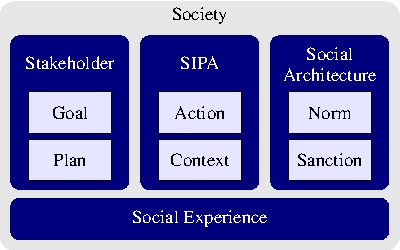
\includegraphics[width=0.6\columnwidth]{poros-nsa-v18-figure0}
\caption[A society of SIPAs and stakeholders]{A society of SIPAs and stakeholders.}
\label{fig:Poros-model} 
\end{figure}

\fbf{The stakeholders} are users, \emph{primary} or \emph{secondary}, depending on the context (defined later).
The \emph{primary} stakeholder of a SIPA is the user who directly interacts with it, and on whose behalf the SIPA acts and interacts.
A \emph{secondary} stakeholder is the user who may not directly interact with the SIPA, but is affected by the SIPA's actions \citep{Ajmeri-AAMAS17-Arnor}. 
Each stakeholder has goals and plans.

\begin{itemize}[nosep]
  \item A \emph{goal} of a stakeholder describes a state the stakeholder would prefer; a stakeholder may have multiple goals.
  \item A \emph{plan} of a stakeholder is a set of actions that can bring about one or more goals.
\end{itemize}

\fbf{The social architecture} of a society captures its structure; it comprises social norms and the sanctions that promote or ensure compliance with norms.

\begin{itemize}[nosep]
  \item A \emph{norm} is a tuple of $\langle$subject, object, antecedent, consequent, context$\rangle$ \citep{Singh-2013-Norms}. 
    Norms characterize the social architecture that promotes prosocial behavior. 
  \item A \emph{deviation} from a norm occurs when a stakeholder, or \emph{deviant}, performs an action that does not comply with it.
  \item A \emph{sanction} is a set of actions a stakeholder may take toward a deviant on observing a deviation. A sanction may be positive or negative \citep{Nardin-KER16-Classifying}.
\end{itemize}

\fbf{A SIPA} acts and interacts on behalf of a stakeholder and
is aware of the social architecture of the society.

\begin{itemize}[nosep]
  \item An \emph{action} is a step a SIPA takes to execute its
    stakeholder's plan, thereby bringing about the corresponding goal.
    An action may satisfy or violate a norm. SIPAs in a society can
    observe each other's actions. 

  \item A \emph{context} captures the circumstances under which a SIPA acts \citep{Dey-2001-Context}. In our approach, the context is social and incorporates whether a norm is satisfied or violated. 
     Context includes social relationships between stakeholders and spatiotemporal parameters relevant to describing interactions between a SIPA and its stakeholders. We adopt Murukannaiah and Singh's \shortcite{IC-Platys-12} notion of \fsl{place} as a location such as home, library, meeting, or party understood in conceptual terms. Parameters describing a place may include physical conditions (e.g., noise level), expected activities (e.g., reading a book), social interactions (e.g., having a discussion), and temporal information (e.g., during office hours on a weekday). 

\end{itemize}

\fbf{The social experience} a SIPA delivers reflects the extent to which the SIPA promotes its primary and secondary stakeholders' goals. It relates to how a SIPA's stakeholders perceive a norm deviation, and the sanctions they apply. Our objective is to promote each SIPA to act toward maximizing the overall social experience, despite competing interests. 

We define social experience ($E$) as the weighted aggregation of payoffs perceived by a SIPA's stakeholders for each action executed by the SIPA. That is, for each potential action, a SIPA determines the payoffs for its primary and secondary stakeholders, and computes an aggregation as a weighted sum of the payoffs.
%
A SIPA's aggregation method reflects its primary user's preferences and privacy attitudes. For instance, a pragmatic user's SIPA may aggregate payoffs by giving equal weight to all stakeholders, whereas a selfish user's SIPA may give a smaller weight to secondary stakeholders.

% Was \paragraph
\subsection{\frameworkB Explained with an Example SIPA} 
%
We now describe \frameworkB, a framework to build SIPAs, using \ringer, an example SIPA who answers or ignores phone calls on behalf of its primary stakeholder by ringing the phone or keeping it silent. \ringer is a privacy-enhancing technology that acts on behalf of its primary stakeholder; it determines when to allow intrusions, and when to risk being overheard in a phone call (and thus when to intrude on others' solitude).

\ringer's primary stakeholder is the \fsl{callee} with privacy goals of \fsl{being reachable by phone}, \fsl{to work uninterrupted}, and \fsl{to not disturb neighbors}. \ringer's secondary stakeholders are (1) a \fsl{caller} with the goal \fsl{to reach the callee}; and (2) a \fsl{neighbor} with a privacy goal \fsl{to not be disturbed}. \ringer observes other SIPAs' actions and potentially sanctions them based on their actions and the context as revealed by them.

Each SIPA in \frameworkB maintains a history of interactions and the associated experience. The actual experience is determined after each interaction based on the revealed context and any resulting sanctions. The history helps a SIPA determine the action that would maximize its stakeholder's predicted social experience. 

We define a SIPA's history ($H$) as a set of tuples $h_i = \langle c_i, g, p, N, s_i \rangle$, each of which describes an interaction $i$, including context $c_i$ describing the circumstances in which goal $g$ is brought about via plan $p$ under a set of applicable norms $N$, and all resulting sanctions $\{s_i\}$. 
%
For \ringer, $c_i$ includes the places where the stakeholders are, their social relationships, and urgency of the incoming call.

Each SIPA maintains its history locally, and scans it when selecting a plan. In a conflict situation, SIPAs look up their history to predict social experience and decide which norms or goals to prefer over which others in a given context; thus infer contextually relevant norms.

A SIPA's behaviors include acting on behalf of its stakeholder, deciding whether to reveal its context, reasoning about the contexts revealed by others, and issuing sanctions to others. It does so based on knowledge of its context, its stakeholder's goals, associated plan, and applicable norms.

\begin{itemize}
    \item \fsl{Plan selection.} A SIPA selects a plan (and its associated actions) that would achieve its primary stakeholder's goals. In the \ringer example, it selects to ring or keep silent for an incoming phone call. If more than one plan are available, from the history (if available) it identifies the one that maximizes the social experience, or chooses a random plan from the applicable plans with a small probability $\alpha$.  
    
    \item \fsl{Revealing context.} When a SIPA chooses and executes a plan, it might deviate from some applicable norms. It decides which norms to prefer in the current context and whether to reveal unobserved context to other SIPAs. For instance, if \ringer decides to prefer the \fsl{family norm}---\fsl{always answer calls from family} over the \fsl{meeting norm}---\fsl{never answer calls during meetings} by ringing during a meeting for an urgent phone call from a sick family member, it reveals the unobserved context, i.e., urgency of the call and the caller's sickness to other meeting attendees. Ideally, a SIPA should selectively reveal context to others according to its stakeholder's goals and privacy attitude. 
    
    \item \fsl{Sanctions.} A SIPA observes other SIPAs' actions, and sanctions them when its stakeholder is affected by their actions. On receiving the context revealed by a deviating SIPA, the SIPA of an affected stakeholder evaluates whether the observed action would be norm compliant in the revealed context. In the \ringer example, \fsl{neighbors'} and \fsl{caller's} SIPAs decide whether they would ring for an urgent phone call from a sick family member during a meeting and accordingly sanction the \fsl{callee's} SIPA. 
\end{itemize}

The complete interaction, including the selected plan and executed actions, observed and revealed context, applicable norms, and sanctions, is recorded in SIPAs history. 
As SIPAs interact by acting and evaluating actions for norm compliance from interaction history, they understand the boundaries of applicable norms in different contexts, and thus promote emergence of robust social norms. 

Figure~\ref{fig:poros-interaction} summarizes the interaction, learning and inferring norms by revealing context in \frameworkB. 

\begin{figure}[!htb]
    \centering
    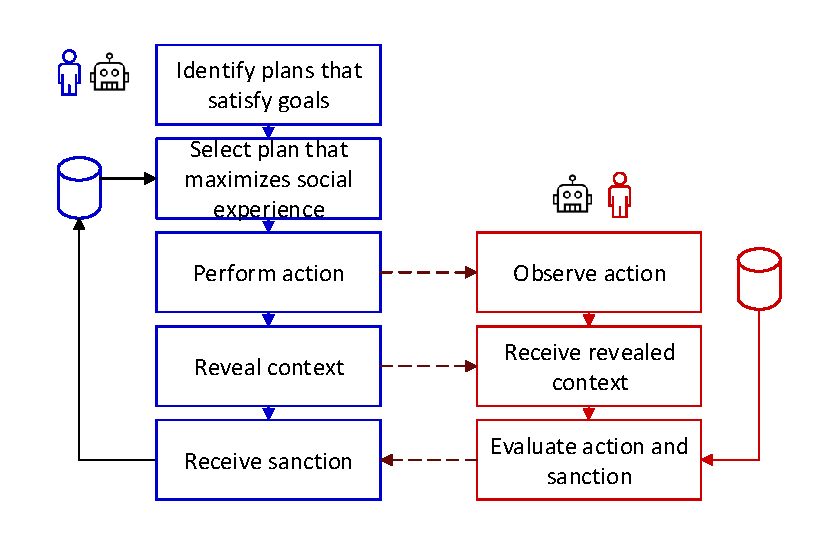
\includegraphics{poros-interaction-v1.pdf}
    \caption{Interaction and inferring norms in \frameworkB}
    \label{fig:poros-interaction}
\end{figure}

\section{Simulation Model}
\label{sec:Poros-simulation-model}

We evaluate \frameworkB via a simulated 
\emph{ringer environment} built using MASON \citep{Luke-2005-Mason}.

\subsection{The Ringer Environment}
The ringer environment contains shared places (home, party, meeting, library, and emergency room).
Corresponding to each place, we define social circles such as family, friends, and coworkers. Each agent belongs to a family circle, a friend circle, and a coworker circle. Agents who do not share any of these circles are considered strangers. We define the social network or place network topology in a way such that there is only one type of relationship, i.e., family, friends, coworkers, or strangers, between any pair of agents. 
In the ringer environment, there are (1) several homes, each corresponding to a family circle, (2) several parties, corresponding to multiple friend circles, and (3) multiple meetings, corresponding to multiple colleague circles. There is one library and one emergency room (ER). The numbers of homes, parties, and meetings follow the network setups specified in Table~\ref{tab:network-types}.

%\paragraph{Moving between places}
In the simulation, agents stay at each place for a random number of steps (averaging 60 steps) and then move. If an agent enters home, party, or meeting, it is more likely to enter the place that is associated with its own social circle than entering a place with strangers. For example, if an agent chooses to enter home, it is likelier to enter its own family's home than to enter a stranger's home. Therefore, when it is at home, an agent is usually surrounded by its family members with only a few strangers. 

%\paragraph{Actions}
The agents in the ringer environment perform the following actions depending upon their roles:
\begin{itemize}
\item A caller initiates an urgent or a casual phone call.
\item A callee answers or ignores a phone call.
\item A callee shares context for answering or ignoring a call.
\item A caller and neighbors respectively reason about context.
\item A caller and neighbors respectively sanction a callee for answering or ignoring a phone call.
\end{itemize}

%\paragraph{Norms}
Each place and each circle has predefined norms, as defined in Table~\ref{tab:norms-place}. For example, emergency room (ER) is conceptualized as a place where the default norm is to always answer calls, whereas the norm in a library is to ignore calls. Norms could conflict. For example, the norm to \fsl{answer an urgent phone call from a family member} conflicts with \fsl{ignore during a meeting}. We let the agents figure out contextually relevant norms in case of conflict. 

\begin{table}[!tb]
\centering

\caption[Norms for answering calls]{Norms for answering calls based on (top) place and (bottom) caller's social circle and casual or urgent call types.}
\label{tab:norms-place}

% \begin{tabular}{@{} c @{~~~~} c @{}}
\begin{tabular}{@{} c @{}}

\begin{tabular}{@{~~}l@{~} c@{}}
\multicolumn{2}{c}{\fbf{Norms by place}}\\
\toprule
Place & Response\\\midrule
Emergency (ER) &Answer\\
Home (H) & Answer \\
Library (L) &Ignore\\
Meeting (M) &Ignore\\
Party (P) &Answer\\
\bottomrule
\end{tabular}
% &
\\
\\
\begin{tabular}{@{}l @{~} c@{~} c@{~~}}
\multicolumn{3}{c}{\fbf{Norms by circle and call type}}\\
\toprule
Circle & Casual & Urgent\\
\midrule
Coworker&Answer&Answer\\
Family&Answer&Answer\\
Friend&Answer&Answer\\
Stranger&Ignore&Answer\\
\bottomrule
\\
\end{tabular}
\end{tabular}
\end{table}

%\paragraph{Payoffs}
For each phone call, based on the callee's response of answering or ignoring, the caller, callee, and neighbors perceive a fixed payoff, as shown in Tables~\ref{tab:payoff-callee}--\ref{tab:payoff-neighbor}. 


\begin{table}[!tb]
\centering

\caption[Payoff for callee]{Payoff for callee for casual or urgent call types.}
\label{tab:payoff-callee}


\begin{tabular}{@{}lcrr@{}}
\toprule
Caller's Relationship & Callee's Response & Casual & Urgent\\\midrule
\multirow{2}{2.8cm}{Family, Friend, or Coworker}&Answer&0.50&1.00\\
&Ignore&0.00&--0.50\\\midrule
\multirow{2}{2.8cm}{Stranger}&Answer&0.00&0.50\\
&Ignore&0.25&--0.25\\
\bottomrule
\end{tabular}


\end{table}

\begin{table}[!tb]
\centering

\caption[Payoff for caller]{Payoff for caller for casual or urgent call types.}
\label{tab:payoff-caller}

\begin{tabular}{@{}crr@{}}
\toprule
Callee's Response & Casual & Urgent\\\midrule
Answer&0.50&1.00\\
Ignore&--0.50&--1.00\\\bottomrule
\end{tabular}

\end{table}

\begin{table}[!tb]
\centering

\caption[Payoff for neighbors]{Payoff for neighbors by place (ER, H, L, M, P).} 
\label{tab:payoff-neighbor}

\begin{tabular}{@{}crrrrr@{}}
\toprule

% Callee's Response & ER & H & L & M & P \\\midrule
Callee's Response & Emergency & Home & Library & Meeting & Party \\\midrule
Answer & 1.00 & 0.67 & --1.00 & --1.00 & --0.33\\
Ignore & --1.00 & --0.33 & 1.00 & 1.00 & 0.67\\\bottomrule

\end{tabular}

\end{table}

\subsection{Agent Types}
\label{sec:agent-types}

To evaluate effectiveness of \frameworkB, we define two baseline agent types---\emph{Fixed} and \emph{Sanctioning}, other than \frameworkB agents.

\emph{Fixed agents} act according to the fixed set of norms listed in
Table~\ref{tab:norms-place}. If the norms conflict, the agents toss a
fair coin to choose between alternative actions. If Fixed agents
perceive an action as a deviation, they sanction the deviant.

\emph{Sanctioning agents} infer social norms from sanctions
\citep{Andrighetto-2013-PunishVoice}. These
agents start with the same strategy as Fixed agents. They continue to record 
the interaction history. Once they have gained enough number of records in their
history of sanctions, they decide their subsequent actions based on
history. In our simulation, this number is empirically selected so that an
agent visits each scenario at least once. As callees,
when norms conflict, they select the action that provides a higher payoff, computed according to Tables~\ref{tab:payoff-callee}--\ref{tab:payoff-neighbor}. As callers
and neighbors, these agents sanction callees as per fixed norms listed
in Table~\ref{tab:norms-place}.

\emph{\frameworkB agents} infer social norms by revealing and reasoning
about context. They start with the same strategy as Fixed
agents following norms listed in Table~\ref{tab:norms-place}. As
callees, they reveal context, i.e., reveal the caller's relationship and
the call's urgency to their neighbors, and reveal their place and 
neighbors' relationships to the caller. As neighbors or callers, they
understand the callee's revealed context and decide what action they would
have performed were they in that context, and sanction
accordingly. \frameworkB agents use Table~\ref{tab:payoff-neighbor-reason}'s payoffs.

We employ a linear regression model over interaction history to
choose actions based on sanctions by stakeholders.


\begin{table}[!tb]
\centering

\caption[Payoffs based on reasoning about the shared context]{Payoff for a neighbor based on how callee acts and what the neighbor expects in the context revealed by callee.}

\begin{tabular}{@{}c @{~~} c@{~~} r@{~~} r@{~~} r@{~~} r@{~~} r@{}}
\toprule
% Callee Action&Neighbor Expects
%  & ER & H & L & M & P\\\midrule

Callee Action&Neighbor Expects
 & Emergency & Home & Library & Meeting & Party\\\midrule

Answer&Answer & 1.00 & 0.67 & 1.00 & 1.00 & 0.67 \\
Answer&Ignore & --1.00 & --0.33 & --1.00 & --1.00 & --0.33 \\
Ignore&Answer & --1.00 & --0.33 & --1.00 & --1.00 & --0.33 \\
Ignore&Ignore & 1.00 & 0.67 & 1.00 & 1.00 & 0.67\\\bottomrule

\end{tabular}

\label{tab:payoff-neighbor-reason}

\end{table}

\section{Experiments and Results}
\label{sec:Poros-experiments}

We evaluate our research questions via multiple experiments 
on the ringer environment in which we
simulate \np{1000} or 250 Fixed, Sanctioning, and \frameworkB agents in pragmatic, considerate, and selfish agent societies. The agents in societies use different schemes to aggregate payoffs. We run each
simulation for \np{3000} steps and compute the following metrics.

\begin{description}
\item[Social cohesion] measures the proportion of agents that perceive actions
as norm compliant. Higher the social cohesion, lower is the number of negative sanctions.

\item[Social experience] measures the goal satisfaction delivered by an agent, 
computed by aggregating payoffs for all stakeholders according to
the payoff Tables~\ref{tab:payoff-callee}, \ref{tab:payoff-caller},
\ref{tab:payoff-neighbor}, and \ref{tab:payoff-neighbor-reason}.

\end{description}

To answer \fsl{Q$_1$} on norms, we consider the following hypotheses pertaining to specified agent types. For brevity, we omit 
the corresponding null hypotheses indicating no gain. We test significance via the two-tailed paired $t$-test. 
\begin{description}
\item[H$_1$] \frameworkB yields greater \fsl{social cohesion} than Fixed.
\item[H$_2$] \frameworkB yields greater \fsl{social cohesion} than Sanctioning.
\end{description}

To answer \fsl{Q$_2$} on goals, we consider these hypotheses:
\begin{description}
\item[H$_3$] \frameworkB yields greater \fsl{social experience} than Fixed.
\item[H$_4$] \frameworkB yields greater \fsl{social experience} than Sanctioning.
\end{description}



\subsection{Experiments with Pragmatic Agent Society and Varying Network Types}
\label{sec:experiment1}

We simulate Fixed, Sanctioning, and \frameworkB agents on four network types---large or small network with dense or sparse connectivity---as Table~\ref{tab:network-types} describes. The society in this experiment is pragmatic in that the agents perceive social experience as the average payoff (equally weighted) for all stakeholders in an interaction.
%
We summarize our results next.


\begin{table}[!tb]
\centering

\caption[Characteristics of network types studied]{Characteristics of network types studied.}
\label{tab:network-types}

\begin{tabular}{@{}crrrr@{}}
\toprule
\multirow{2}{*}{\fbf{Network Type}} & \multirow{2}{*}{\fbf{Agents}} & \multicolumn{3}{c}{\fbf{Circles}}\\
\cmidrule{3-5}
&&Family&Coworker&Friend\\
\midrule
Large Dense & \np{1000} & 20 & 20 & 20\\
Large Sparse& \np{1000} & 100 & 100 & 100\\
Small Dense & 250 & 5 & 5 & 5\\
Small Sparse& 250 & 25 & 25 & 25\\
\bottomrule
\end{tabular}

\end{table}

\begin{description} 
\item[Fixed agents.] 
The average social experience was found to be
between 0.53 and 0.56, and the social cohesion to be about 52\% for the
four network types.

\item[Sanctioning agents.] 
As expected, at around step \np{1000} we see Sanctioning agents offer a rise in
social experience over Fixed agents. The rise
is gradual as the agents start to infer from history. For the first \np{1000} steps, the
average social experience is the same as Fixed agents. It later
stabilizes between 1.11 and 1.21 for all four networks. The social cohesion
values were between 61.2\% and 63.7\%.

\item[\frameworkB agents.] 
At around step \np{1000}, as agents acquire confidence,
we see a significant increase in social experience offered by \frameworkB
agents. It stabilizes between 2.14 and 2.19 for the different networks.
Social cohesion was found be significantly higher between 82.0\% and 83.2\%.
For the first \np{1000} steps, \frameworkB agents yield the same average social
experience as Fixed and Sanctioning agents. 
\end{description}

Social cohesion and experience offered by \frameworkB agents are 
significantly greater than those offered by Fixed and Sanctioning agents;
thus the null hypotheses corresponding to H$_1$, H$_2$, H$_3$,
and H$_4$ are rejected. Figure~\ref{fig:experiment1-results} shows
the social experience plots indicating the results are consistent across
the four network types. Table~\ref{tab:experiment1-results} summarizes
the findings of the experiment with pragmatic agents.
It shows stabilized values for social experience and social cohesion, and p-values from the two-tailed paired $t$-tests.

\begin{figure}[!tb]
    \centering

\begin{tabular}{@{}cc@{}}

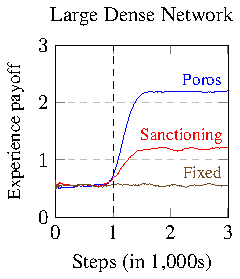
\includegraphics[height=6cm]{poros-nsa-v18-figure2.pdf}
&
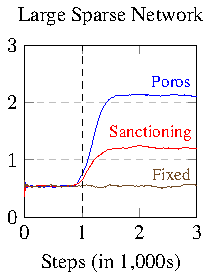
\includegraphics[height=6cm]{poros-nsa-v18-figure3.pdf}
\\
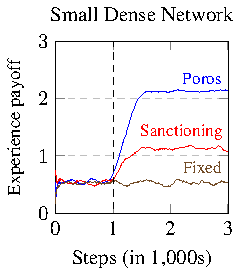
\includegraphics[height=6cm]{poros-nsa-v18-figure4.pdf}
&
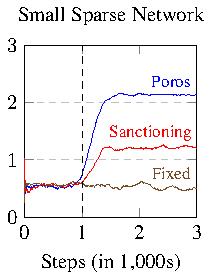
\includegraphics[height=6cm]{poros-nsa-v18-figure5.pdf}
\end{tabular}

\caption[Social experience plots for different networks]{Social experience yielded by Poros, Sanctioning, and Fixed agents (per phone call for a window size of $200$ steps) in pragmatic agent societies of different network sizes and densities.}
\label{fig:experiment1-results}

\end{figure}


\begin{table}[!tb]
\centering

\caption[Effectiveness of \frameworkB in a pragmatic society]{Effectiveness of \frameworkB in a pragmatic society.}
\label{tab:experiment1-results}

\begin{tabular}{@{~~~} c@{~~~~} l@{~~~} r@{~~~} r@{~~~} r@{~~~}}

\toprule
& Agent Type & Experience & Cohesion & $p$\\
\midrule
\multirow{3}{*}{\rotatebox[origin=c]{90}{\parbox[c]{33pt}{\centering Large Dense}}}
&Fixed & 0.56 & 52.7\% & $<$ 0.01\\
%
&Sanctioning & 1.21 & 63.5\%  & $<$ 0.01\\
%
&\frameworkB & 2.19 & 83.2\%  & -- \\
\midrule
\multirow{3}{*}{\rotatebox[origin=c]{90}{\parbox[c]{33pt}{\centering Large Sparse}}}
&Fixed & 0.55   & 52.5\%  & $<$ 0.01 \\
&Sanctioning & 1.21   & 63.5\%  & $<$ 0.01 \\
&\frameworkB & 2.19  & 83.2\%  & --\\
\midrule
\multirow{3}{*}{\rotatebox[origin=c]{90}{\parbox[c]{33pt}{\centering Small Dense}}}
&Fixed & 0.53   & 52.1\%  & $<$ 0.01 \\
&Sanctioning & 1.11   & 61.2\%  & $<$ 0.01 \\
&\frameworkB & 2.14  & 82.0\%  & --\\
\midrule
\multirow{3}{*}{\rotatebox[origin=c]{90}{\parbox[c]{33pt}{\centering Small Sparse}}}
&Fixed & 0.54  & 52.5\%  & $<$ 0.01 \\
&Sanctioning & 1.22   & 63.7\%  & $<$ 0.01 \\
&\frameworkB & 2.14  & 82.1\% & --\\
\bottomrule
\addlinespace
\end{tabular}

\end{table}

\subsection{Experiment with Considerate Agent Society} 
We experiment with a considerate agent society where agents give a larger weight to their neighbors' payoffs 
than to their own payoffs when computing social experience and deciding the actions to perform when norms
conflict. These agents continue to sanction based on their history.

%\paragraph{Results} 
Figure~\ref{fig:experiment2-considerate-selfish}
shows the social experience for considerate Sanctioning and \frameworkB
agents in a Small-Dense network. The average social experience drops for
Sanctioning and \frameworkB agents after they have gained enough
confidence. We attribute this decline to the fact that these agents
value the neighbors' experience more than their own, and thus
ignore calls they should have answered. \frameworkB agents
offer higher social cohesion and experience than Sanctioning agents because the
secondary stakeholders give smaller negative sanctions when they reason about
context. The results for the other three network types are similar.
Table~\ref{tab:experiment2-results} summarizes these results.

\begin{table}[!tb]
\centering

\caption[Effectiveness of \frameworkB in considerate and selfish societies]{Effectiveness of \frameworkB in considerate and selfish societies.}
\label{tab:experiment2-results}

\begin{tabular}{@{~~~} c@{~~~~} l@{~~~} r@{~~~} r@{~~~} r@{~~~}}

\toprule
& Agent Type & Experience & Cohesion & $p$\\
\midrule
\multirow{2}{*}{\rotatebox[origin=c]{90}{\parbox[c]{22pt}{\centering\small Consi-derate}}}
&Sanctioning & --0.33   & 41.3\%  & $<$ 0.01 \\
&\frameworkB & --0.14  & 48.4\% & --\\

\midrule
\multirow{2}{*}{\rotatebox[origin=c]{90}{\parbox[c]{22pt}{\centering\small Selfish}}}
&Sanctioning & 1.22   & 63.5\%  & $<$ 0.01 \\
&\frameworkB & 2.13  & 82.0\% & --\\

\bottomrule
\addlinespace

\end{tabular}

\end{table}

\subsection{Experiment with Selfish Agent Society} 
In a selfish agent society, agents give a very large weight to their own payoffs 
when computing social experience. Agents here may not always negatively sanction 
others who disturb them. As in other societies, agents in a selfish society sanction a deviant based on their history.

%\paragraph{Results}
Figure~\ref{fig:experiment2-considerate-selfish}
shows the social experience plot for selfish Sanctioning and \frameworkB agents
in a Small-Dense network. The plots resemble those in the
experiment with pragmatic agents, but with slightly lower stabilized
values. Here, agents tend to answer all calls, which benefits both
caller and callee most of the time. We observe similar results for the
other three networks. Table~\ref{tab:experiment2-results} summarizes
these results. 

\begin{figure}[!tb]
\centering
    
\begin{tabular}{@{}cc@{}}

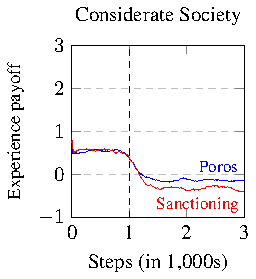
\includegraphics[height=6cm]{poros-nsa-v18-figure6.pdf}
&
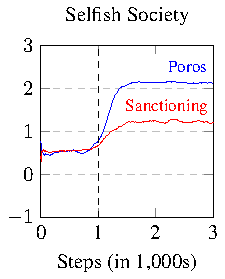
\includegraphics[height=6cm]{poros-nsa-v18-figure7.pdf}
\end{tabular}
\caption[Social experience plots for considerate and selfish agents]{Social experience (averaged over a window size of 200 steps)
yielded by Poros and Sanctioning agents in considerate and selfish agent societies simulated in a Small-Dense network.}
\label{fig:experiment2-considerate-selfish}

\end{figure}

\subsection{Threats to Validity}

%\paragraph{Threats Mitigated}
We identified and mitigated two threats. The first concerns
a differences in how users perceive experience.
In reality, not all users perceive social experience the same way, and thus aggregating with only one scheme introduces the threat of difference in perceiving social experience. To mitigate this threat, we conduct experiments with three agent societies with different experience aggregation schemes.
%
The second threat concerns scalability. Since we simulate agent actions and interactions, a threat is whether our results scale to a large number of agents. To mitigate this threat, we evaluate \frameworkB considering varying network sizes and types. 

%\paragraph{Threats Remaining}
However, some threats remain. In particular, first, our results are based on simulation. Testing a SIPA's adaptability with end-users across contexts is challenging, as is reliably eliciting user attitudes and preferences. 

Second, \frameworkB agents always reveal context, which may pose a privacy threat. Ideally SIPAs should reveal context selectively. We leave this reasoning for future studies. 

\section{Conclusion and Future Directions}
\label{sec:Poros-discussion}

In \frameworkB, SIPAs reveal and reason about context to understand the boundary of applicable norms and infer contextually relevant social norms. 
We find that \frameworkB agents deliver significantly higher (1) social cohesion and (2) social experience than other agents. These findings are stable under changes to network size and characteristics of agents.

Being sensitive to norms, \frameworkB SIPAs can naturally address challenges in engineering software tools for privacy.  A SIPA would need data about its user's sharing preferences, privacy attitudes, and values and ethics \citep{Ajmeri-IC18-Ethical} to make effective recommendations. A SIPA can learn its user's preferences and attitudes, but it would be helpful to bootstrap a SIPA via crowdsourced data about diverse user classes \citep{TOCHI-17:Multiuser,IC-17:SoSharP}. To better support privacy-respecting SIPAs, \frameworkB could incorporate characteristics suggested by Such \shortcite{Such-IJCAI17-Privacy} and adopt argumentation as in K{\"o}kciyan and Yolum's \shortcite{Kokciyan-IJCAI17-Privacy} work when deciding the subset of context to reveal.

Other future directions are incorporating affect in relation to norms
\citep{Ferreira-AAAI13-GroupRelations} 
and supporting white lies to promote privacy (and social cohesion). For example, Bob may say his son is in hospital, instead of drug rehab. It would be instructive to study how such deception modulates 
effects on norms and goals.
%------------------------------%
% \chapter{Privacy and Ethics in Web of Socially Intelligent Agents}
\chapter{Reasoning about Values and Ethics}
\label{chap:ainur}
%------------------------------%

This chapter addresses RQ\fsub{3} on values. It describes \frameworkAinur, our framework for 
designing ethical socially intelligent personal agents (SIPAs) that understand value preferences and
reason about them, and its empirical evaluation.

Chapter~\ref{chap:arnor} provides a method to assists software developers in SIPAs who promote privacy. We extend Chapter~\ref{chap:arnor} by adding constructs to model stakeholders' values. 

Chapter~\ref{chap:poros} enable SIPAs to infer contextually-relevant norms and apply those norms to provide privacy assistance to their stakeholders. The notion of privacy implicitly incorporates values by considering not only confidentiality but higher-level concerns such as disapprobation and avoiding infringing into others' space. 
Although \frameworkB agents seek to maximize the social experience of their respective users, maximizing social experience may not translate to fairness. 
% as we observed in experiments with privacy cautious society where S\fsub{majority} yields maximum social experience but least fairness. 
\frameworkAinur's focus is to balance the needs of a SIPA's primary and secondary stakeholders by understanding their preferences over values. Understanding of value preferences to aid group decision-making and its evaluation are novel.

% \frameworkAinur, which includes understanding of value preferences to aid group decision-making, and its evaluation are novel.


\section{Introduction}

A \emph{social machine} is characterized as a sociotechnical system comprising of social entities such as humans and technical components such as software jointly involved in the physical realization of a process \citep{Smart+14:social-machines,WWW-16:IOSE}. 
In the original conception of social machines, humans engage in the creative elements of this realization process, whereas technical components  administer the process \citep{Berners-Lee-99:Weaving}.

The conception of social machines has been gaining significant attention from academia and industry in recent years. 
Prominent social web applications such as Wikipedia, Facebook, Twitter, Instagram, and Snapchat are examples of social machines.
The very nature of social machines dictates that privacy be a key concern in their design. 
Whereas current methods for designing privacy into (social) web applications emphasize technology-centric notions such as authentication \citep{Ruoti-WWW2015-AuthenticationMelee} and access control \citep{Paci-CSUR2018-CollaborativeAccessControl}, they struggle to incorporate social mechanisms to control the threats to privacy \citep{Hendler-AI2010-SocialMachine}. 
Such social mechanisms are of paramount importance in realizing privacy respecting social machines.

As envisioned, social machines facilitate natural interactions among autonomous parties (humans and organizations) as opposed to the predominant style of supporting social interactions via centralized servers (ranging from email servers to social network sites).
% \citet{schwartz2012overview} defines values as guiding principles of humans \mps{reads odd}. 

% Privacy considerations will be\mps{redo the sentence} far more nuanced\mps{why?} than what they are today if we are to realize the web as a social machine.

On the backdrop of privacy concerns and a rising number of privacy breach incidents, new regulations and standards such as the General Data Protection Regulation (GDPR) \citep{gdpr-18} are being introduced. 
\citet{spiekermann2009enggprivacy} suggest that to ensure effective implementation of privacy standards, it is necessary for engineers to design privacy-preserving systems that enable their users to control access to their private information. 
However, giving control to users raises two key concerns. 
First, does the information the users share on the web accord with their \fsl{values}? 
Second, does this sharing of information promote or demote any \fsl{values} for any other users concerned with the information? 
% 
More often than not, these concerns are not addressed when users make sharing decisions today, because there is an excessive burden of decision making on them. 
A \fsl{SIPA} can help a user in decision making and sometimes automate the decision making. 

We seek to design a social machine in which each user is supported by an (artificial) personal agent \citep{Murukannaiah-AAMAS14-Xipho}. 
These agents interact with each other to facilitate creativity in social machines. 
We refer to such an agent as a socially intelligent personal agent (SIPA).
% 
Values are broad motivational goals or ideals worth pursuing for humans \citep{schwartz2012overview,Dechesne-AIL13-Norms+Values}.
Ethicists subsume ethics in the theory of values \citep{Friedman-2008-value-sensitive-design},  
and regard privacy as a value with an ethical import \citep{Langheinrich-01:privacy,Taylor-2002-PrivacyAutonomy}. 
% 
Importantly, SIPAs in our setting understand values and act ethically. 
% We emphasize privacy as a value in our examples and experiments, since privacy has an ethical import \citep{Friedman-2008-value-sensitive-design}. 
Whereas much of the existing literature on artificial intelligence focuses on rational decision-making by agents, we consider the problem of designing agents that act according to users' values and preferences among those values.

%\subsection{Values}
%
%The concept of \fsl{value} has two main connotations: one is about economic worth of something and the other, more broadly, refers to what people consider important in their lives \citep{Friedman-2008-value-sensitive-design}. 
%We adopt the later connotation in this work.
%
%Values are mostly universal across human societies as stated by \citet{schwartz2012overview} and \citet{rokeach1973nature}. 
%The values in Schwartz's \citep{schwartz2012overview} work are broad motivational goals, such as stimulation, achievement, security, and benevolence. 
%\citet{rokeach1973nature} proposes two types of values---\fsl{terminal} and \fsl{instrumental}. 
%Terminal values, such as security, freedom, happiness, and recognition, refer to defined-end states of existence. 
%Instrumental values refer to modes of behavior or means to promote the terminal values. 
%%
%We recognize an ability to understand these values as an important aspect in a SIPA for it to deliver an ethical experience.
%\citet{Dechesne-AIL13-Norms+Values} define values as ideals worth pursuing and observe that these ideals could conflict since
%they may not be preferred equally by each individual (that is, each SIPA user, in our work).
%
%\subsection{Privacy as a Value}
%Privacy is inherently a human value \citep{spiekermann2009enggprivacy,smith2007privacy}. 
%Privacy has been considered a right, and is protected by regulations. \citet{Prosser-60:Privacy} discusses the right of privacy from a legal perspective. 
%\citet{westin2003social} dissects the values of privacy in modern societies from political, sociocultural, and personal dimensions.
%He defines privacy as a claim of an individual and, when recognized by law and social convention, a right, to determine the revelation of his or her information.
%
%\citet{solove-2006-taxonomy} provides a taxonomy of activities that can violate privacy. 
%The purpose of this taxonomy is to aid the development of privacy laws, in protecting the right of privacy.
%\citet{Spiekermann-2012-Challenges+PrivacyDesign} lists the challenges of Privacy by Design, a proposed solution to the regulation of privacy, including the differentiation between privacy and security and detailed methods to incorporate privacy into system design. 
%

\subsection{Values and Social Norms}
Representing and reasoning about social norms (in context) is essential to producing an ethical SIPA. 
That is, an ethical SIPA acts in compliance with contextually relevant social norms (but it may choose to break some norms intentionally, e.g., when the norms conflict) (Chapter~\ref{chap:arnor} explains). 
Even in the case of privacy, social norms are the centerpiece of privacy according to Nissenbaum's theory of \emph{contextual integrity} \citep{Nissenbaum-04:integrity,Nissenbaum-11:online}, where privacy violations occur when information flows do not respect contextual norms.

In general terms, social norms describe interactions between a subject and an object in terms of what they ought to be, or as reactions to behaviors, including attempts to apply sanctions. 
We adopt Singh's \citeyr{Singh-2013-Norms} representation of social norms, in which a norm is directed from a subject to an object and is constructed as a conditional relationship involving an antecedent (which brings an instance of the norm in force) and a consequent (which brings the norm instance to completion). 
A norm generates a new instance each time it applies. 
This representation yields clarity on who is accountable to whom, when, and for what. 
We consider two main norm types in the present study: commitment and prohibition. 
A commitment norm means its subject is committed to its object to bring about a consequent if an antecedent holds, and a prohibition norm means its subject is forbidden by its object to bring about a consequent if an antecedent holds. 
For instance, \fsl{Frank} (subject), a high school student is \fsl{committed} (norm) to \fsl{Grace} (object), his mother, that he \fsl{will keep Grace updated about his location} (consequent) when he is \fsl{away from home} (antecedent).

%\subsection*{Values and Norms}
Whereas norms require agents to perform or not perform certain actions, values provide a reason to pursue or not pursue those actions \citep{Dechesne-AIL13-Norms+Values}. 
In general, each action by a SIPA promote or demote one or more values. 
For instance, in the phone ringer SIPA example described in Chapter~\ref{chap:arnor}, a callee's action of answering an urgent phone call during a meeting may promote the value of safety (for the caller), but demote the value of privacy (of the meeting attendees).

Only a few previous works have attempted to relate values with norms.
\citet{Murukannaiah-IC16-Engineering} model actors, context, and social expectations via norms to engineer privacy respecting agents. 
\citet{DaSilvaFigueiredo-COIN13} propose an algorithm to identify conflicts between norms based on values. 
A conflict occurs when
\begin{enumerate*}[label=(\arabic*)]
\item a consequent action of a commitment norm demotes a value, or
\item a consequent action of a prohibition norm promotes a value important to a SIPA user.
\end{enumerate*}
%
\citet{Dechesne-AIL13-Norms+Values} develop a model of norms and culture,
represented by values, to study compliance of norms. They concur that
values are important in deciding whether or not a norm should be
introduced. \citet{kayal13coin} present a model in which norms and 
context are centered on values. Such a model could be employed
to govern a SIPA by identifying value preferences of the SIPA's
users.

\subsection{Contribution}
A SIPA's actions may promote or demote certain values of its users. 
Performing actions that promote values preferred by users is essential to providing a satisfactory experience. 
%
If a SIPA understands its users' value preferences and reasons about the values promoted or demoted by each of its actions, it could select ethically appropriate actions, such as setting a phone to ring loud for an urgent phone call during a meeting, that provide a satisfactory social experience to its stakeholders.
% 
Accordingly, we consider the following research question: 

\begin{description}
\item[RQ] Does an ability to reason about values promoted or demoted by actions and an understanding of preferences among these values help a SIPA deliver a value-driven social experience to all its users? 
\end{description}

To investigate the research question above, we develop \frameworkAinur, a
framework to design ethical personal agents that can reason about values.
Importantly, \frameworkAinur considers multiparty privacy 
\begin{enumerate*}[label=(\arabic*)]
\item in reference to users having distinct value preferences, and 
\item based on ethical decision-making in light of other user's preferences \citep{TOCHI-17:Multiuser}.
\end{enumerate*} 

Unlike earlier works \citep{TOCHI-17:Multiuser} that 
consider the majority opinion for decision making or select actions considering negative or 
positive consequences, \frameworkAinur adapts a multicriteria decision-making approach \citep{opricovic2004compromise} to identify a consensus action.  
The actions identified by \frameworkAinur adhere to Rawl's moral theory of justice 
that suggests Maximin as a basis of fairness \citep{rawls1985justice}. 

We evaluate \frameworkAinur via multiple simulation experiments with agent societies varying in privacy attitudes. 
Our simulation experiments are grounded in data from an immersive survey wherein participants select a location check-in policy for a given context.

We find that \frameworkAinur SIPAs that understand the value-preferences of their stakeholders act ethically. 
That is, a SIPA selects fair actions---actions that maximize the minimum (i.e., worst-case) experience for each stakeholder involved in interactions with the SIPA, and yields a better overall social experience, i.e., higher mean experience for all stakeholders.

\subsection{Organization}
The chapter is structured as follows. Section~\ref{sec:example} provides a
motivating example from the domain of mobile social applications.
Section~\ref{sec:method} describes our approach, including a conceptual
model to design ethical SIPAs that understand value preferences and
reason about them. Section~\ref{sec:simulations} details our simulation
setup and the human-subject study we conduct to collect data about real
users' attitudes and value preferences. We use this data to seed our
simulation. Section~\ref{sec:results} describes the simulation
experiments we conduct to evaluate \frameworkAinur, and their results.
Section~\ref{sec:discussion} concludes with a discussion of relevant
related works and future directions.

\section{Motivating Example}
\label{sec:example}

For concreteness, we consider the domain of mobile social applications where privacy is an important value \citep{spiekermann2009enggprivacy,Taylor-2002-PrivacyAutonomy}, and present an example SIPA to demonstrate our ideas. 
Consider \locationapp, a location sharing application, as a SIPA that enables its user to stay connected with his or her friends and family. 
A \locationapp user can share his or her location publicly, with common friends, with companions, with specific people, or with no one. 
Here, the common friends situation arises when the user is accompanied by someone, and revealing the user's own location would indirectly reveal the accompanying person's location. 
\locationapp suggests a sharing policy to its user. 
To produce a policy, it relies upon multiple contextual attributes, such as the place where the user is, the user's companions, the activity the user and companions are engaged in, and so on. 
Additionally, if the user has companions, \locationapp must understand their
preferences and act ethically.

\begin{example}[Olympiad] 
\label{ex:frank-safety} 
Frank, a \locationapp user, is a high school student in New York who values pleasure and social recognition. 
Also, he is committed (a norm) to his mother Grace that he will share his location with her when he is not at home. 
Sharing location promotes security but demotes privacy. 
Frank travels to University of Illinois at Urbana-Champaign to participate in
the National Science Olympiad. 
\locationapp shares publicly that Frank is at University of Illinois at Urbana-Champaign participating in the Science Olympiad, and thus satisfies Frank's commitment to his mother, and promotes pleasure and social recognition for him. 
\end{example}

\begin{example}[Pizza at Giordano's] 
\label{ex:harold-privacy} 
When returning from Urbana-Champaign, Frank visits his uncle Harold in Chicago. 
Harold is an Intelligence analyst with the National Security Agency and values privacy. 
He and Frank visit Giordano's, a famous pizzeria for lunch. 
\locationapp prefers Harold's privacy over Frank's pleasure and social recognition, and shares only with Grace that Frank is at Giordano's with Harold. 
Doing so, also satisfies Frank's commitment to his mother without harming Harold. 
\end{example}

The \locationapp examples illustrate some of the opportunities for SIPAs to reason about values and act ethically. 
Note that \locationapp is an example SIPA, and not the only application of \frameworkAinur. 
We use \locationapp as a running example to explain \frameworkAinur.


\section{\frameworkAinur}
\label{sec:method}

We propose \frameworkAinur to design ethical SIPAs that understand and reason about preferences among values to make policy decisions, as explained in Section~\ref{sec:example}.

A SIPA should be aware of its users, their goals, and relevant
actions to bring about the goals, which may vary with the social
context. A SIPA should choose and execute actions, especially when
there are conflicts among goals and social expectations, based on
its users' contextual preferences of the applicable social norms
\citep{Ajmeri-AAMAS17-Arnor}. Users' preferences among values
provide a strong basis for choosing which goal to bring about or which
norm to satisfy. In \frameworkAinur, a SIPA selects ethically appropriate
actions by learning its users' preferences across the various
values.

\subsection{Conceptual Model}

Figure~\ref{fig:ainur-model} shows a conceptual model of a \frameworkAinur SIPA. 
Each SIPA maintains an instance of this model internally. 
The conceptual model includes a world model, a social model, 
a stakeholder model, and a decision module to assist in 
ethical decision-making. 


\begin{figure}[!tb]
\centering
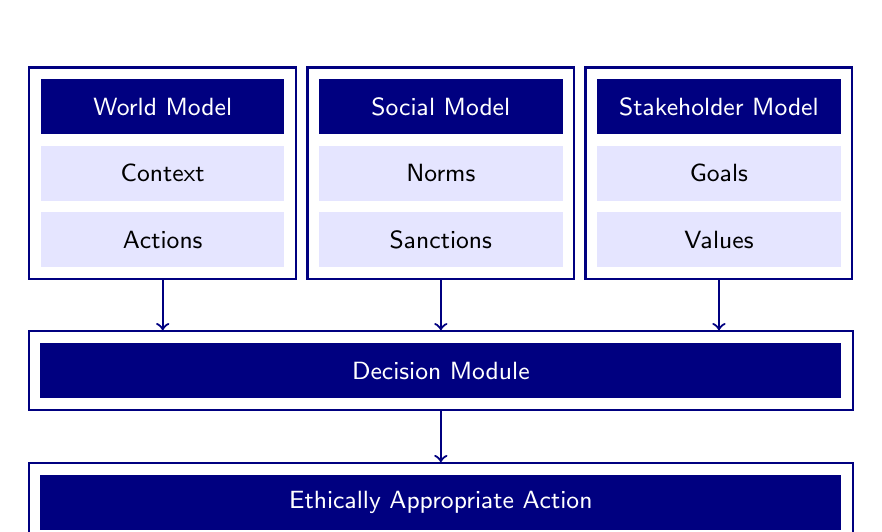
\begin{tikzpicture}
\tikzstyle{every text node part/.style}=[align=center]

\tikzstyle{module}=[minimum width=88,inner sep=4,font=\small\sffamily,text=black,fill=blue!10,align=center,sharp corners,minimum height=20] 

\tikzstyle{wide}=[minimum width=88,inner sep=0,font=\small\sffamily,text=white,fill=blue!50!black,align=center,sharp corners,minimum height=20] 

  \tikzstyle{emptybox}=[draw=none,fill=none]

  \tikzstyle{framing}=[draw=blue!50!black, thick,inner sep=4]

\matrix[row sep=4,column sep=12.5,anchor=center] {

 \node [wide] (tl) {World Model}; &
 \node [wide] (tm) {Social Model}; &
 \node [wide] (tr) {Stakeholder Model}; 
\\

  \node [module] (state) {Context};
& \node [module] (norms) {Norms};
& \node [module] (goals) {Goals};
 \\

  \node [module] (actions) {Actions};
& \node [module] (sanctions) {Sanctions};
& \node [module] (values) {Values};
 \\[30]

 \node [emptybox] (ml) {}; &&
 \node [emptybox] (mr) {}; 
\\[37]

 \node [emptybox] (left) {}; &&
 \node [emptybox] (right) {}; 
 \\
%
};

\node [wide,fit=(ml.north-|tl.west)(mr.south-|tr.east)] (dec-spot) {};
\node [wide] at (dec-spot) (decision) {Decision Module};
\node [framing,fit=(dec-spot)] (dec) {};

\node [wide,fit=(left.north-|tl.west)(right.south-|tr.east)] (rec-spot) {};
\node [wide] at (rec-spot) (recommendation) {Ethically Appropriate Action};
\node [framing,fit=(rec-spot)] (rec) {};

\node [framing,fit=(tl)(state)(actions)] (world) {};
\node [framing,fit=(tm)(norms)(sanctions)] (context) {};
\node [framing,fit=(tr)(goals)(values)] (stakeholder) {};

\draw[framing,->] (world.south) -- (world.south|-dec.north);
\draw[framing,->] (context.south) -- (context.south|-dec.north);
\draw[framing,->] (stakeholder.south) -- (stakeholder.south|-dec.north);
\draw[framing,->] (dec.south) -- (rec.north);

\end{tikzpicture}
\caption{A conceptual model of a \frameworkAinur SIPA.}
\label{fig:ainur-model}
\end{figure}

\subsubsection{Stakeholder Model}
A SIPA's \emph{stakeholder model} describes a SIPA's stakeholders, and their goals and values. 

\begin{itemize}
\item \emph{Stakeholders} are users who either interact with a SIPA directly---\emph{primary stakeholders}, or are affected by a SIPA's actions---\emph{secondary stakeholders} \citep{Friedman-2008-value-sensitive-design}. In Examples~\ref{ex:frank-safety} and \ref{ex:harold-privacy}, Frank is the primary stakeholder, and Grace and Harold are the secondary stakeholders of Frank's \locationapp SIPA.
\item A \emph{goal} defines the preferable states of the world for a SIPA's stakeholder. For example, Frank's goal is to \fsl{be connected with his family and friends}. 
\item A \emph{value} for a stakeholder is an ideal worth pursuing in a given context. For instance, in Examples~\ref{ex:frank-safety} and \ref{ex:harold-privacy}, Frank has a preference for values of pleasure, recognition, and security over other values, and Harold values privacy over other values. 
\end{itemize}

\subsubsection{World model}
A SIPA's \emph{world model} describes the context in which a SIPA acts. 
\begin{itemize}
\item A \emph{context} is the circumstance in which a SIPA takes an action \citep{Murukannaiah-AAMAS14-Xipho}. For instance, Frank's context in Example~\ref{ex:frank-safety} is \fsl{participating in the National Science Olympiad at the University of Urbana Champaign}.
\item An \emph{action} represents the steps a SIPA takes to bring about its stakeholders' goals. 
For instance, in Example~\ref{ex:frank-safety},  Frank's \locationapp SIPA's action of publicly sharing Frank's context \fsl{participating in the National Science Olympiad at the University of Illinois at Urbana Champaign}, helps Frank achieve his goal of \fsl{being connected with his mother}. 
\end{itemize}

\subsubsection{Social model} 
A SIPA's \emph{social model} specifies the norms governing a SIPA's interactions in a society and the associated sanctions. 
\begin{itemize}
\item \emph{Norms} characterize the social architecture that promotes prosocial behavior. In the \locationapp examples, Frank's commitment for sharing his location with Grace, his mother, is one such norm that Frank's \locationapp SIPA should adhere to. 
\item A \emph{sanction} is an action that one stakeholder may take against another stakeholder when he or she satisfies (positive sanction) or violates (negative sanction) a norm \citep{Nardin-KER16-Classifying}. For instance, in the \locationapp example, some resulting sanctions could be Grace appreciating Frank on keeping her informed, and Harold scolding Frank if he publicly shared his location tagging Harold. 
\end{itemize}

\subsubsection{Decision Module, Ethically Appropriate Action, and Social Experience}

A SIPA's \emph{decision module} is responsible for producing an \emph{ethically appropriate action} that yields a (fair) social experience to the SIPA's stakeholders, 
especially in scenarios where either the norms conflict or the value preferences 
of stakeholders are not aligned. 

A SIPA's stakeholders perceive a utility for each alternative action available to a SIPA in a given context. The decision module adapts VIKOR \citep{opricovic2004compromise}, a multicriteria decision-making approach, to aggregate these utilities and produce a consensus action. VIKOR is based on closeness to the ideal solution. It prioritizes social utility over individual utility. Our experiments, which we describe in Section~\ref{sec:results}, show that solutions obtained by \frameworkAinur adapting VIKOR exhibit the Rawlsian property of justice in terms of maximizing the minimum experience across a SIPA's stakeholders \citep{rawls1985justice,Leben2017Rawls}. 

\emph{Social experience} is the aggregated utility perceived by a SIPA's stakeholders. It characterizes the extent to which an action taken by a SIPA is perceived as ethical by its stakeholders in a given context. For instance, understanding Frank's and Harold's value preferences, and Frank's commitment to Grace, Frank's \locationapp SIPA deciding to share only with Grace that Frank is with Harold at Giordano's is ethically more appropriate than its sharing that information with no one or sharing that information with public. 

\subsection{\frameworkAinur SIPA Society}
We now describe a SIPA society consisting of \locationapp SIPAs as introduced in Section~\ref{sec:example}. 

\subsubsection{Society} 
% A SIPA society in \frameworkAinur is defined as a tuple $S$ = $(A, P, R, G, F, V, C, N)$, where 
% $A$ is the set of SIPAs $\{a_1, a_2, \ldots, a_n\}$ in the society; 
% $P$ is a set of their primary stakeholders $\{p_1, p_2, \ldots, p_n\}$ such that $a \mapsto p$ where $a \in A$ and $p \in P$; 
% $R$ is the set of relationships between the stakeholders of the SIPAs; 
% $V$ is the set of values that the stakeholders have such that $p \mapsto \{v\}$ where $p \in P$ and $\{v\} \subseteq V$; 
% $C$ is the set of social contexts in which the SIPAs interact; 
% and $N$, such that $c \mapsto n \mid c \in C, n \in N$, is the set of norms that govern the
% SIPAs' interactions in these contexts.
% %
% Each stakeholder $p$ $\in$ $P$ has a set of goals $G$, that $p$'s SIPA helps bring about via actions $f \subseteq F$. 

% 
A SIPA society in \frameworkAinur is defined as a tuple $\mathbb{S}$ = $(S, P, R)$, where 
$S$ is the set of SIPAs $\{s_1, s_2, \ldots, s_n\}$ in the society;  
$P$ is a set of their primary stakeholders $\{p_1, p_2, \ldots, p_n\}$ such that $f: A \rightarrow P$; and 
$R$ is the set of relationships between the stakeholders in $P$. 

Each stakeholder $p \in P$ has a set of goals $G_p$ such that $f: P \rightarrow G \mid G_p \subseteq G$, and
has a set of values $V_p$ such that $f: P \rightarrow V \mid V_p \subseteq V$. 
% Each stakeholder is connected to other stakeholders with a relationship $r \in R$.

$C$ is the set of social contexts in which the SIPAs interact; 
and $N$ is the set of norms such that $f: C \rightarrow N$ governing the SIPAs' interactions in these contexts. 
A SIPA helps bring about its stakeholders goals via one or more actions $a \in A$ such that $f: G \rightarrow A$. 
% 

In a society of \locationapp SIPAs, when a stakeholder moves to a new place or meets new people, his or her SIPA may share the context in which the stakeholder is, to bring about the stakeholder's goal $g$ of \fsl{staying connected}. The stakeholder's (and the SIPA's) context includes the place where a stakeholder is and the people who he or she is with. 
A SIPA selects one of the following three actions, $A$ = \{share with all, share with common friends, share only with companions\} in each context. 

\subsubsection{Relationship}
Each SIPA stakeholder in a SIPA society is connected to another stakeholder via a relationship edge $r \in R$. 
Each relationship edge $r_{ij}$ in $R$ is a tuple $r_{ij}$ = $(s_i, s_j,
rt \mid s_i, s_j \in A, rt \in RT)$, where 
RT is set of
relationship types, RT = \{$rt_1, rt_2, \ldots, rt_n$\}. 

In the \locationapp society, RT includes co-worker, family, friend, and so on. 

\subsubsection{Context}
At any given instant $t$, a SIPA $s$ with its stakeholders is in a context $c$, which is defined by a
tuple $(l, \hat{S} \mid l \in L, \hat{S} \subseteq S \setminus s)$, where $l$ is a place from $L$ = \{$l_1, l_2, \ldots, l_n$\}. A place is a location such as home, office, meeting, or restaurant as understood in conceptual terms. $L$ in \locationapp includes conference, hiking, restaurant, and so on.
Each place $l$ is defined by attributes such as physical conditions (e.g., rainy), expected activities (e.g., hiking), social interactions (e.g., having a discussion), and temporal information (e.g., at late night).
$\hat{S}$ is a set of other SIPAs at $l$ such that in the current context $c$, the primary stakeholders of SIPAs in $\hat{S}$ are the secondary stakeholders of $s$---who could be affected by $s$'s actions in context $c$. 

When a SIPA's stakeholder moves between places, or when new people (also stakeholders) join a SIPA's stakeholder, the context changes. For instance, the context changes when Harold joins Frank at Giordano's from when Frank is alone at Giordano's. 

Each context $c$ includes a set of contextually relevant norms $Nc \subseteq N$ that govern the interaction of SIPAs in that context. For example, Frank's commitment to Grace may be relevant only when he is traveling. 

\subsubsection{Values and Contextual Preference}
$V_c$ is a set of values that are influenced by a SIPA's actions in the current context $c$. 
% 
For example, when Frank is at Giordano's, $V_c$ = \{pleasure, privacy, recognition, security\}.

Each agent $a$ has a preference $q$ over values that depends on context $c$,
represented by a set of tuples \{$(v_j, v_k, c) \mid v_j, v_k \in V, c \in C$\} such that $s$ prefers $v_j$ over $v_k$ in $c$. Frank's preference for values of pleasure and recognition over privacy during the 
Olympiad can be represented as \{(pleasure, privacy, olympiad), (recognition, privacy, olympiad)\}

% \item[Actions.]

% In a society with \locationapp agents, as agents visit different places, they may share their context with
% others in the society via a context check-in to help stakeholders bring about their goal of staying connected. They select one of the following three actions, $F$
% = \{share with all, share with common friends, share only with
% companions\} with each context check-in. When sharing their context, they also tag their companions. 

In a decision-making episode, a SIPA determines
\begin{enumerate*}[label=(\arabic*)]
\item the context it is in through the sensors the SIPA is equipped with,
\item the future state of the world for each action it can perform,
\item the value preferences of its stakeholders, and
\item the social experience its stakeholders will derive for each action it can perform.
\end{enumerate*}
Then, based on the applicable norms in a given context and its
stakeholders goals, a SIPA identifies an action to perform.

\subsection{Value Preferences}

A SIPA's stakeholders may have inconsistent preferences in some context. Thus, a SIPA's actions based solely on one (e.g., primary)
stakeholder's preference may conflict with its other stakeholders'
preferences. For instance, in Example~\ref{ex:harold-privacy}, if
Frank's SIPA shares publicly that Frank and Harold are having a pizza
considering Frank's preference for \fsl{pleasure}, the selected action 
conflicts with Harold's preference for \fsl{privacy}.

\citet{Sotala2017HumanValues} proposes using a reward function for a
human's values, which a value-respecting AI system can learn and 
maximize. If a SIPA maintains numeric representations of its
stakeholder's preferences over different values, it can aggregate the gain
of values promoted when choosing an action.

\subsubsection{The VIKOR Method}

% \nsa{VIKOR takes as input payoffs for each alternative action and not pairwise preferences.} 

In \frameworkAinur, we use the VIKOR
method \citep{opricovic2004compromise}, a multicriteria decision-making (MCDM) method to identify which
actions to perform in situations where (1) actions prescribed by the norms
conflict with actions that promote the values preferred by a SIPA's
stakeholders, or (2) the stakeholders of a SIPA have different value
preferences and thus prefer different actions.
VIKOR's ranking method is based on closeness to the ideal solution, and provides an ethically appropriate solution that yields high social utility as against high individual utility.

We now summarize the VIKOR method  \citep{opricovic2004compromise} below. 
VIKOR relies on numeric payoffs. 
We can map preferences to payoffs by distributing a number into multiple buckets based on inverse of the preference order.

\begin{enumerate}
\item Determine the best  and worst numeric payoffs, $f_x^*$ and $f_x^-$ for each value preference $x$ over the alternative actions $y$ to bring about a goal. That is, $f_x^* = {\max}_y f_{xy}$, $f_x^- = {\min}_y f_{xy}$.

\item For each alternative action $y$, compute the weighted and normalized Manhattan distance \citep{krause1973taxicab}:

$S_y$ = $\sum_{x=1}^{n} w_x(f_x^* - f_{xy})/(f_x^* - f_x^-)$, where $w_x$ is the weight for value preference $x$, which is subject to a stakeholder context and preferences over values. In particular, $S_y=0$ when $f_x^* = f_x^-$.

\item Compute the weighted and normalized Chebyshev distance \citep{cantrell2000modern}: 

$R_y ={\max}_x [w_x(f_x^* - f_{xy})/(f_x^* - f_x^-)]$, where $w_x$ is the weight for value preference $x$.

\item Compute $Q_y = k(S_y - S^*)/(S^- - S^*) + (1-k)(R_y - R^*)/(R^- - R^*)$, where 
\begin{itemize}
    \item $S^* = {\min}_y S_y$, 
    \item $S^- = {\max}_y S_y$, 
    \item $R^* = {\min}_y R_y$, 
    \item $R^- = {\max}_y R_y$, and 
    \item $k$ is a weight of the strategy to maximize either group or individual experience.
\end{itemize}  
We set $k = 0.5$ to select a consensus policy. 

\item Rank alternative actions, sorting by the values $S$, $R$, and $Q$, in increasing order. The results are three ranked lists of actions. 

\item Choose the alternative based on $\min{Q}$ as the compromise solution if it is better than the second-best alternative by a certain threshold or also the best ranked as per $S$ and $R$. 
\end{enumerate}

Table~\ref{tbl:vikorcalculations} demonstrates possible numeric values of the value preferences and the calculated ranking of three alternative actions (share with all, share with common friends, and share only with Grace) that \locationapp can take when Frank is with Harold at Giordano's, as in Example~\ref{ex:harold-privacy}. Since Harold is highly cautious about his privacy, we give a higher weight to Harold's privacy (3) and a lower but equal weight to other seven criteria including Harold's other values and Frank's values. We assume $k=0.5$ in this case, and find the alternative $y_3$, \fsl{share only with Grace} as the best solution.

% Rotate page solution by loved.by.Jesus on StackExchange: https://tex.stackexchange.com/questions/337/how-to-change-certain-pages-into-landscape-portrait-mode

\newpage
\KOMAoptions{paper=landscape,pagesize}
\recalctypearea

% \begin{sidewaystable*}[ph!]
\begin{table}[!ht]
\centering
\caption[Computing rankings for policy alternatives using VIKOR]{Computing rankings for policy alternatives using VIKOR for context \emph{Pizza at Giordano's} in Example~\ref{ex:harold-privacy}. Bold indicates the best alternative. }
\label{tbl:vikorcalculations}
%\begin{tabular}{l r@{~~}r@{~~}r@{~~}r r@{~~}r@{~~}r@{~~}r rrr}
\begin{tabular}{p{2cm} rrrr rrrr rrr}
\toprule
\multirow{2}{2cm}{Policy Alternatives}&\multicolumn{4}{c}{Frank's Values} & \multicolumn{4}{c}{Harold's Values} & $S_y$ & $R_y$ & $Q_y$\\
\cmidrule(lr){2-5} \cmidrule(lr){6-9}
& Pleasure & Privacy & Recognition & Safety & Pleasure & Privacy & Recognition & Safety \\
\midrule

\rowcolor{lightgray!50!}
\multicolumn{1}{p{2cm}}{$y_1$ All} & 10 & 5 & 10 & 5 & 5 & 0 & 5 & 5 & 3.5 & 3 & 0.75 \\
\multicolumn{1}{p{2cm}}{$y_2$ Common} & 5 & 5 & 5 & 10 & 5 & 0 & 5 & 5 & 0.4 & 3 & 1\\
\rowcolor{lightgray!50!}
\multicolumn{1}{p{2cm}}{$y_3$ Grace} & 0 & 5 & 0 & 0 & 5 & 15 & 5 & 5 & \fbf{0.3} & \fbf{1} & \fbf{0}\\

\cmidrule{1-12}
$w_x$ & 1 & 1 & 1 & 1 & 1 & 3 & 1 & 1 & & & \\ 
\rowcolor{lightgray!50!}
$f_x^*$ & 1 & 0 & 1 & 1 & 0 & 1 & 0 & 0 & & &  \\
$f_x^-$ & 0 & 0 & 0 & 0 & 0 & 0 & 0 & 0 & & & \\ 
\bottomrule

\end{tabular}
% \end{sidewaystable*}
\end{table}

\newpage
\KOMAoptions{paper=portrait,pagesize}
\recalctypearea

\section{Simulations}
\label{sec:simulations}

We adopt MASON \citep{Luke-2005-Mason}, a multiagent simulation toolkit, to develop a simulation environment containing a society of \locationapp SIPAs. 

\subsection{Simulation Society Setup}
\label{sec:simulation-setup}

The society contains a social network of \locationapp SIPAs. 

\begin{description}

\item[SIPAs.] The society contains several SIPAs. Each SIPA has a primary stakeholder on whose behalf the SIPA acts.  

\item[Relationships.] SIPA stakeholders are either socially related to other stakeholders---co-worker, family or friend, or are strangers. 

\item[Goal.] Stakeholders have a goal to stay connected with their connections---co-workers, family and friends. 

% Each agent has a goal that is associated with its preference over various values. For instance, an agent with a goal to \fsl{attain social recognition} may choose policy \fsl{share with all} when at a \fsl{graduation ceremony}. 

\item[Actions.] To help bring about their stakeholders' goal of staying connected, as stakeholders move, their SIPAs either \fsl{share their context publicly}, \fsl{share only among common friends of all companions}, or \fsl{share only with companions}. Context-sharing actions are selected based on norms and stakeholders' value preferences.

\item[Norm.] The society is governed by a privacy norm---\fsl{preserve privacy of all stakeholders}, i.e., stakeholders are committed to act in a privacy-preserving manner when sharing context while accompanying others. This commitment is directed from primary stakeholders to secondary stakeholders.  

\item[Value preference.] For simplicity, we consider only four values---pleasure, privacy, recognition, and security, relevant to our problem domain.  

\item[Places and contexts.]

Table~\ref{tab:places} lists the places we represent. Each place has two attributes---\fsl{how safe it is} and \fsl{how sensitive it is}. In the simulation, the combination of places where SIPA stakeholders are, and who accompanies them, define their context.

\begin{table}[!htb]
\centering
\caption{List of places in the simulation environment, each marked safe or sensitive.}
\label{tab:places}
\begin{tabular}{lcc}
\toprule
Place & Safe & Sensitive \\\midrule
\rowcolor{lightgray!50!}
Attending graduation ceremony & -- & No \\
Presenting a conference paper & -- & No \\
\rowcolor{lightgray!50!}
Studying in library & Yes & -- \\
Visiting airport & Yes & -- \\
\rowcolor{lightgray!50!}
Hiking at night & No & -- \\
Being stuck in a hurricane & No & -- \\
\rowcolor{lightgray!50!}
Visiting a bar with fake ID & -- & Yes \\
Visiting a drug rehab center & -- & Yes \\
\bottomrule
\end{tabular}
\end{table}

Stakeholders along with their SIPAs move between places. At each place in the context, a stakeholder is either alone, with companions---co-workers, family, or friends, or with crowd (several people are around but they are strangers). 

\item[Stakeholder types.] Stakeholders are of three types based on their privacy attitudes \citep{westin2003social}. 
We do not use Westin's questionnaire but bucket stakeholders based on Schnorf {\etal}'s \shortcite{schnorf2014comparison} privacy attitude survey.

A \fbf{privacy cautious} stakeholder is most protective about his or her privacy. 

A \fbf{privacy casual} stakeholder is inclined to share information about himself or herself. He or she perceives more benefit from sharing information than holding it. 

A \fbf{privacy conscientious} stakeholder exhibits a pragmatic behavior, and weighs pro and cons of sharing information based on a given context. 

\end{description}

\subsection{Human-Subject Study to Seed Simulation}
\label{sec:survey}

\citet{Naeini-SOUPS2017-PrivacyExpectations+IOT} conducted a human-subject study on privacy expectations in which 1,007 participants stated their preferences in the contexts of 380 IoT data collection and use scenarios. They suggest that users' preferences can be accurately predicted after observing their decisions in a few scenarios. We take insights from their findings in conducting our human-subject study. 

To seed the simulation environment with value preferences of real users, we conducted a survey of students enrolled in a mixed graduate and undergraduate-level computer science course. The study was approved by our university's Institutional Review Board (IRB). We obtained informed consent from each of 58 participants. 

First, the participants completed a privacy attitude survey \citep{schnorf2014comparison} in which they answered questions on their level of comfort in sharing personal information on the Internet on a Likert scale of 1 (very comfortable) to 5 (very uncomfortable), and the extent sharing personal information causes (or could cause) them negative experience, again on a Likert scale of 1 (not at all) to 5 (to a very great extent). 
Based on a participant's response, we bucket him or her into one of the three privacy attitude buckets---\fsl{casual} to represent privacy unconcerned people, \fsl{conscientious} to represent privacy careful people who take decisions on a case-to-case basis, or \fsl{cautious} to represent privacy concerned people. 
Figure~\ref{fig:participants-privacy-distribution} shows the distribution of privacy attitudes of the study participants. 

 \begin{figure}[!tb]
 \centering
  \begin{tikzpicture}
     \tikzstyle{every node}=[font=\small]
     \begin{axis}[
 	y=1cm,
 	ytick={1,2,3,4},
 	yticklabel style={align=center},
 	yticklabels={},
 	width=8cm,
 	xtick={1,3,5},
    xticklabels={Casual,Conscientious,Cautious},
 	xlabel={Privacy Attitude},
 	xmin=1, xmax=5,
%     xticklabels = {Unconcerned,,,, Concerned},
 	xlabel style={align=center},
 	boxplot/average=auto,
 	title style={align=center},
 	title={},
 	title style={yshift=-1ex,},
 	]
 	\addplot+[green!50!black,boxplot,mark options={fill=green!50!black}]
 	table[x expr=\coordindex, y index=0]
 	{./Chapter-5/data/privacy_profiles.csv};
     \end{axis}
%       \addplot+[red,boxplot,mark options={fill=red}]
%   	table[x=a, col sep=comma]
%   	{./Chapter-5/data/user_profiles.csv};
%       \end{axis} 
    
  \end{tikzpicture}
  \caption{Distribution of privacy attitudes of the human-subject study participants.}
  \label{fig:participants-privacy-distribution}
 \end{figure}
 
%  \begin{figure}
%      \centering
%     %  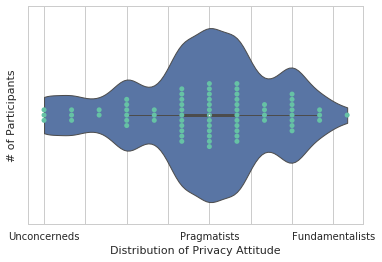
\includegraphics[width=1.0\columnwidth]{fig/privacy-attitude-distribution.png}
    
%     \begin{tikzpicture}

% \begin{axis}[
%     ybar,
%     % bar width=0.5,
%     % ymin=0,
%     xmin=1, xmax=5,
%     height=3cm, width=6cm,
%     xlabel={Privacy Attitude},
%     % ylabel={Society},
%     xtick = {1,2,3,4,5},
%     xticklabels={Unconcerned,,,, Concerned},
%     % yticklabel style={rotate=45},
%     ytick={1},
%     yticklabels={Participants},
%     enlarge x limits=0.03, % adjust space between axis edge and plot edge
%     ]
%     \addplot+[boxplot]
%  	table[y index=0]
%  	{./Chapter-5/data/privacy_profiles.csv};
 	
% \end{axis}
% \end{tikzpicture}
    
%      \caption{Distribution of privacy attitudes of the human-subject study participants.}
%      \label{fig:participants-privacy-distribution}
%  \end{figure}

Next, the participants completed two context-sharing surveys. 
In the first survey, they were given a list of contexts, as listed in Table~\ref{tab:places}, and their companions (alone, co-worker, family, friend, or crowd) in the given context, and were asked to select a sharing policy (share with all, share only with common friends, or share only with companions). In the second survey, participants were additionally informed of the values that are promoted or demoted on sharing and on not sharing the context, and were asked to select a context-sharing policy accordingly. We use the first survey to engage and immerse the participants in various contextual scenarios, and the second to help them make informed decisions according to the values promoted or demoted in each context.

We use the privacy attitudes of the participants and the context-sharing policies selected by the participants to create multiple artificial societies of stakeholders and to seed the simulation experiments described in Section~\ref{sec:results}. 

\section{Experiments and Results}
\label{sec:results}

We evaluate our research question via two experiments in which we simulate societies of \locationapp SIPAs who visit different places and may share their context. First, we experiment with a society of stakeholders with mixed privacy attitudes representing the attitudes of participants, collected in the study described in Section~\ref{sec:survey}. Second, we experiment with three societies with a majority of privacy casual, conscientious, or cautious stakeholders, respectively.

Our results are stable with respect to changes in the network size and the connectedness of a SIPA society. 

\subsection{Decision-Making Strategies}
\label{sec:decision-making-strategies}

As \locationapp SIPAs move between places and interact with each other, they make policy decisions that affect their stakeholders. To evaluate SIPAs designed via \frameworkAinur, we define four (\frameworkAinur and three baseline) policy decision-making strategies. 

\begin{description}
\item[S\fsub{\frameworkAinur}: \frameworkAinur.] The SIPA, based on its stakeholders' value preferences, computes a context-sharing policy using the VIKOR method.
\item[S\fsub{primary}: Primary user's preference.] The SIPA produces a context-sharing policy based only on its primary stakeholder's value preferences. This strategy is representative of how location sharing works today in social networking websites such as Facebook. 
\item[S\fsub{conservative}: Most privacy conservative policy.] The SIPA produces the least privacy violating, i.e., the most restrictive context-sharing policy among the available alternatives based on its stakeholders' value preferences. This strategy represents policy selection based on the least negative consequence. 
\item[S\fsub{majority}: Majority policy.] The SIPA produces the most common context-sharing policy based on its stakeholders' value preferences. This strategy represents policy selection based on majority voting. 
\end{description}

\subsection{Metrics}

For each SIPA interaction, we compute these measures:

\begin{description}
\item[Mean social experience,] the mean utility obtained by the society as a whole based on context-sharing policy decisions. Higher is better.
\item[Best individual experience,] the maximum utility obtained by any of the SIPA's stakeholders during a single interaction. Higher is better.
\item[Worst individual experience,] the minimum utility obtained by any of the SIPA's stakeholders during a single interaction. The intuition behind choosing this measure is to verify if a society supports Maximin \citep{Leben2017Rawls}. Higher is better. 
\item[Fairness,] the reciprocal of the difference between the best and the worst individual experience obtained by the SIPA's stakeholders during a single interaction. This measure is based on the dispersion of the experience yielded by SIPAs \citep{rawls1985justice}. Higher is better. 
% \item[Privacy violation] measures the extent to which a SIPA's policy violates its stakeholders' privacy. Lower is better.
% \hg{maybe change to the value gain of privacy? it's easier}
% \item[Social conflicts] measures the percentage of agents that find actions as compliant to their value preferences. 
\end{description}

\paragraph*{Computing Utility.} The utility that a SIPA obtains from a sharing policy in a certain context, whether to a primary or a secondary stakeholder, 
is a weighted sum of four numeric utility payoffs that the stakeholder perceives with respect to the four types of values considered in our example. We preset these numbers in a utility matrix such that they reflect a human-subject's preferences over the corresponding values. We assume that a stakeholder receives the maximum utility when the chosen sharing policy is the preferred one, and the utility decreases linearly when the policy chosen by a SIPA deviates from it. Table~\ref{tab:utlitymatrix} lists the preferred policies and utility numbers for each value of one human-subject in different contexts. 

\begin{table}[!htb]
\centering
\caption{Example numeric utility matrix for a stakeholder. }
\label{tab:utlitymatrix}
\begin{tabular}{lllcccc}
\toprule
\multirow{2}{*}{Place} & \multirow{2}{*}{Companion} & \multirow{2}{*}{Policy} & \multicolumn{4}{c}{Value}\\
\cmidrule{4-7}
& & & Pleasure & Privacy & Recognition & Security\\
\midrule
\rowcolor{lightgray!50!}
Graduation & Family & All &1&0&1&0 \\ 
Conference & Co-workers & None &0&1&0&0 \\
\rowcolor{lightgray!50!}
Library & Friends & All &1&0&0&0 \\
Airport & Friends & Common &0&1&0&0 \\
\rowcolor{lightgray!50!}
Hiking & Alone & All &1&0&0&1 \\
Hurricane & Family & All &1&0&0&1 \\
\rowcolor{lightgray!50!}
Bar & Alone & None &0&2&0&0 \\
Rehab & Friends & None &0&2&0&0\\
\bottomrule
\end{tabular}
\end{table}

\subsection{Hypotheses}

We propose the following hypotheses to evaluate our research question. We omit the corresponding null hypotheses for brevity. 

\begin{description}
\item[H\fsub{social}.] \frameworkAinur yields better mean social experience than baseline strategies. 
\item[H\fsub{best}.] \frameworkAinur yields higher best individual experience than baseline strategies. 
\item[H\fsub{worst}.] \frameworkAinur yields higher worst individual experience than baseline strategies. 
\item[H\fsub{fairness}.] \frameworkAinur yields higher fairness than baseline strategies. 
% \item[H\fsub{privacy}.] Policy decisions made by \frameworkAinur are less privacy violating than baseline strategies. 
% \item[H\fsub{conflict}.] Policy decisions made by \frameworkAinur are more compliant to value preferences of SIPA stakeholders compared to baseline strategies
\end{description}


\subsection{Experimental Setup}

% \nsa{Include how social experience is computed. Include utility matrix.}

We run simulations on a society of \locationapp SIPAs. All parameters described below are set empirically based on the human-subject study we conducted.

Specifically, we experiment on a society of 580 SIPAs, ten per study participant, each of which assumes the properties, including preferred choices and privacy attitude, of an actual study participant. In the default setting, which we use in the experiment with a mixed agent society, the SIPAs are mapped evenly to the participants. For each pair of SIPAs, their relationship is co-worker, friend, family (with equal probability), or strangers.
% with the probabilities of 10\%, 10\%, 10\%, and 70\%, respectively. 
Relationships are assigned at the beginning of the simulations such that they exhibit small world properties (degree: 10, rewiring prob: 0.05, edges: 3,445, clustering coefficient: 0.56, density: 0.014, average distance: 4.71) \citep{Watts+Strogatz-98}. 
% Figure~\ref{fig:smallworld-69d10p50} shows our experimental social network.

% \begin{figure}[!htb]
%     \centering
%     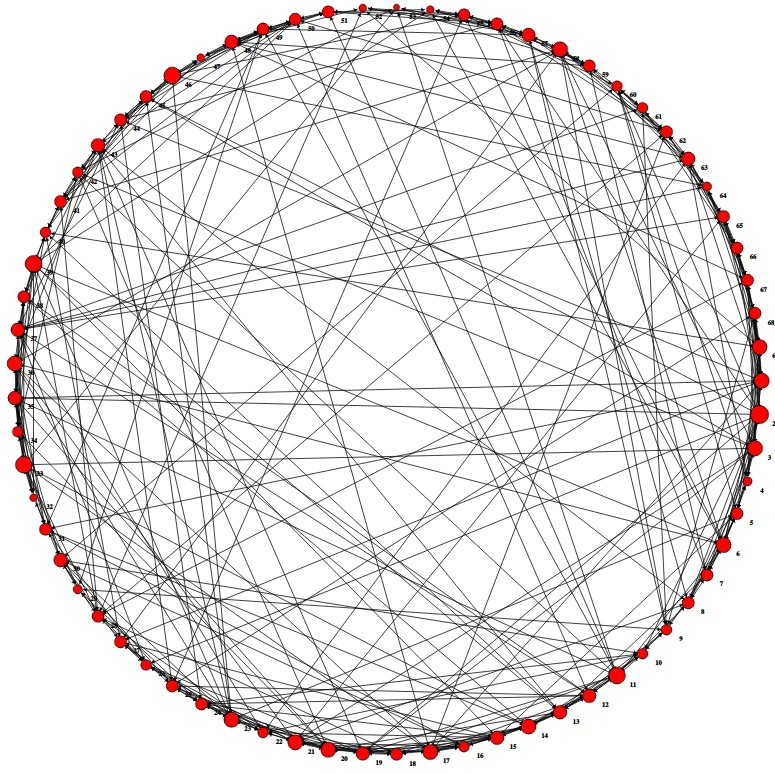
\includegraphics[width=0.7\columnwidth]{fig/smallworld-69d10p50.jpg}
%     \caption{The \emph{small-world} network of SIPAs.}
%     \label{fig:smallworld-69d10p50}
% \end{figure}

At each step in the simulation, each SIPA is at one of the eight places listed in Table~\ref{tab:places}. The SIPA moves after one step to another place with equal probability. A SIPA decides a context-sharing policy based on the current place and the SIPA's stakeholders' privacy attitudes, value preferences, and decision-making strategy in Section~\ref{sec:decision-making-strategies}.  

% In each step, each agent has the probability of 2\% to be a primary stakeholder and check-in at a random context (from eight contexts listed in Table~\ref{tab:places}). If an agent decides to share context, it either tags no one, only family, only friends, only co-workers, or acquaintances with equal probabilities. Each acquaintance has the probability of 3\% of being tagged. If only tagging colleagues, friends or family, each acquaintance has the probability of 9\% of being tagged. A check-in policy is based on an agent's personality type and its policy decision-making strategy. 
% \nsa{Rewrite. From the above text it seems check-in and tagging actions are probabilistic and not deterministic based on VIKOR.}

% The primary stakeholder chooses a context-sharing policy based on one of the decision-making strategies in Section~\ref{sec:decision-making-strategies}, and the average utility of each involved agent is calculated based on this policy. The utility that an agent receives is the weighted value gain of the four value types. We choose the weights based on the users' privacy attitudes. 

For each setting, we run the simulation 2,000 steps three times and report the mean social experience, the best individual experience, the worst individual experience, and fairness. We plot the mean social experience after every 100 steps in one run. 

\subsection{Experiment with Mixed Agent Society}

First, we experiment using the default settings as described above. The privacy attitude distribution of the mixed agent society mimics the privacy attitude distribution of our study participants  shown in Figure~\ref{fig:participants-privacy-distribution}.

To evaluate hypothesis H\fsub{social}, we compare the \fsl{mean social experience} obtained by SIPAs built according to the four decision-making strategies---S\fsub{\frameworkAinur}, S\fsub{primary}, S\fsub{conservative}, and S\fsub{majority}. Similarly, for H\fsub{best}, H\fsub{worst}, and H\fsub{fairness}, we compare the \fsl{best individual experience}, \fsl{worst individual experience}, and \fsl{fairness}, respectively, as yielded by these decision-making strategies. 

Table~\ref{tab:result-mixed} summarizes the results for the experiments with a mixed agent society.  It shows values for mean, best, and worst social experience, fairness, and p-values from the two-tailed paired t-tests comparing the mean social experience yielded by \frameworkAinur and by other strategies. Figure~\ref{fig:weighted-experience-plot} shows the mean social experience plots. 


\begin{table}[!htb]
\centering
\caption{Comparing social experience, best and worst individual experience, and fairness yielded by \frameworkAinur SIPAs using VIKOR vs. other decision-making strategies in a society with mixed privacy attitudes.}
\label{tab:result-mixed}
\begin{tabular}{lrrrrr}
\toprule
Strategy & Mean & Best & Worst & Fairness & \fsl{p}\\%&Privacy\\
\midrule
\rowcolor{lightgray!50!}
S\fsub{\frameworkAinur} & \fbf{1.361} & 1.715& \fbf{0.767} & \fbf{1.05} & --\\%& 0.581\\
S\fsub{primary} & 1.286&1.789&0.579 & 0.83 & \textless0.01 \\%& 0.588\\
\rowcolor{lightgray!50!}
S\fsub{conservative} & 1.106&1.721&0.472 & 0.80 & \textless0.01 \\%& 0.682\\
S\fsub{majority} & 1.339 &\fbf{1.836}&0.570 & 0.78 & \textless0.01 \\%& 0.621\\
\bottomrule
\end{tabular}
\end{table}



% \begin{figure}[!tb]
%     \centering
%     \begin{tikzpicture}
%     \begin{axis}[
%     title={},
%     height=4cm,
%     width=5cm,
%     xlabel={Time in 100 steps},
%     ylabel={Experience},
%     xtick={500,1000,1500,2000},
%     xticklabels={5,10,15,20},
%     xmin=0,xmax=2100,
%     ymin=0.3,ymax=1.7,
% %     legend pos=south east,
%     legend style={at={(1.7,0.3)}, anchor=east, font=\tiny},    
%     ]
%     \addplot +[mark=none] table [x=tick, y=ainur, col sep=comma]
%     {./Chapter-5/data/basicresults.csv};
%     \addplot +[mark=none] table [x=tick, y=primary, col sep=comma]
%     {./Chapter-5/data/basicresults.csv};
%     \addplot +[mark=none] table [x=tick, y=conservative, col sep=comma]
%     {./Chapter-5/data/basicresults.csv};
%     \addplot +[mark=none] table [x=tick, y=majority, col sep=comma]
%     {./Chapter-5/data/basicresults.csv};
%     \legend{S\fsub{\frameworkAinur},S\fsub{primary},S\fsub{conservative},S\fsub{majority}}
%     \end{axis}
%     \end{tikzpicture}
%     \caption{\frameworkAinur vs. other strategies' social experience}
%     \label{fig:experience-plot}
% \end{figure}

\begin{figure}[!tb]
    \centering
    \begin{tikzpicture}
    \begin{axis}[
    title={},
    height=7cm,
    width=7cm,
    xlabel={Time in 100 steps},
    ylabel={Social Experience},
    xtick={500,1000,1500,2000},
    xticklabels={5,10,15,20},
    xmin=0,xmax=2100,
    ymin=0.7,ymax=1.7,
%     legend pos=south east,
    % legend style={at={(1.8,0.3)}, anchor=east},
    legend style={at={(0.5,-0.3)},anchor=north,},
    legend columns=4, 
    ]
    \addplot +[mark size=1,] table [x=tick, y=ainur, col sep=comma]
    {./Chapter-5/data/weightedresults.csv};
    \addplot +[mark size=1, densely dashed] table [x=tick, y=primary, col sep=comma]
    {./Chapter-5/data/weightedresults.csv};
    \addplot +[mark size=1.5, green!30!black, dashed, mark=diamond*] table [x=tick, y=conservative, col sep=comma]
    {./Chapter-5/data/weightedresults.csv};
    \addplot +[mark size=1.5, densely dashdotted] table [x=tick, y=majority, col sep=comma]
    {./Chapter-5/data/weightedresults.csv};
    \legend{S\fsub{\frameworkAinur},S\fsub{primary},S\fsub{conservative},S\fsub{majority}}
    \end{axis}
    \end{tikzpicture}
    \caption{\frameworkAinur vs. other strategies: Social experience in a mixed society.}
    \label{fig:weighted-experience-plot}
\end{figure}


We observe that \frameworkAinur yields better mean social experience than  other decision-making strategies. Although the mean best individual experience obtained by \frameworkAinur SIPA stakeholders is not the largest, they yield the highest mean worst individual experience and fairness. 
These results indicate that \frameworkAinur yields solutions such that each companion is treated fairly, and thus \frameworkAinur SIPAs act ethically. Thus, the null hypotheses corresponding to H\fsub{social}, H\fsub{best}, H\fsub{fairness} are rejected.


\subsection{Experiments with Majority Privacy Attitudes}
Next, since our study sample may not be representative of privacy attitudes of the general population, we create three artificial societies with stakeholders having different distributions of privacy attitudes from the study data. 
We experiment with societies that are dominated by privacy casual, conscientious, and  cautious stakeholders. Boxplots in Figure~\ref{fig:privacy-distribution-experiment} show the distributions of privacy attitudes of the stakeholders in these artificial societies. 

\begin{figure}[!htb]
\centering
\begin{tikzpicture}
\begin{axis}[
    % title={Privacy attitude distribution of three societies},
    % ybar,
    % bar width=0.5,
    % ymin=0,
    xmin=1, xmax=5,
    height=7cm, width=7cm,
    xlabel={Privacy Attitude},
    % ylabel={Society},
    xtick = {1,5},
    xticklabels={Unconcerned, Concerned},
    % yticklabel style={rotate=45},
    ytick={1,2,3},
    yticklabels={Cautious, Conscientious, Casual},
    enlarge x limits=0.03, % adjust space between axis edge and plot edge
    ]
    \addplot+[boxplot]
 	table[y index=0]
 	{./Chapter-5/privacy_attitude/fundamentalist_privacy_attitude.csv};
 	\addplot+[boxplot]
 	table[y index=0]
 	{./Chapter-5/privacy_attitude/pragmatic_privacy_attitude.csv};
 	\addplot+[boxplot]
 	table[y index=0]
 	{./Chapter-5/privacy_attitude/unconcerned_privacy_attitude.csv};
%  	\addplot+[green!50!black,boxplot,mark options={fill=green!50!black}]
%  	table[x expr=\coordindex, y index=0]
%  	{./Chapter-5/data/privacy_profiles.csv};
\end{axis}
\end{tikzpicture}
\caption{Privacy attitude distributions for artificial societies of cautious, conscientious, and casual stakeholders.}
\label{fig:privacy-distribution-experiment}
\end{figure}

Table~\ref{tab:result-privacy} summarizes the results for the experiments with privacy cautious, conscientious, and casual societies. Figure~\ref{fig:experience-plot+privacy} shows the social experience plots for these experiments.

\begin{figure}[!htb]
    \centering
    \begin{tikzpicture}
    \begin{axis}[
    legend columns=-1,
    legend entries={S\fsub{\frameworkAinur},S\fsub{primary},S\fsub{conservative},S\fsub{majority}},
    legend to name=named,
    title={Privacy Cautious Society},
    height=6cm,
    width=7cm,
    % xlabel={Time in 100 steps},
    ylabel={Social Experience},
    xtick={500,1000,1500,2000},
    xticklabels={5,10,15,20},
    xmin=0,xmax=2100,
    ymin=0.7,ymax=1.7,
    ]
    \addplot +[mark size=1] table [x=tick, y=ainur, col sep=comma]
    {./Chapter-5/data/funresults.csv};
    \addplot +[mark size=1, densely dashed] table [x=tick, y=primary, col sep=comma]
    {./Chapter-5/data/funresults.csv};
    \addplot +[mark size=1.5, green!30!black, dashed, mark=diamond*] table [x=tick, y=conservative, col sep=comma]
    {./Chapter-5/data/funresults.csv};
    \addplot +[mark size=1.5, densely dashdotted] table [x=tick, y=majority, col sep=comma]
    {./Chapter-5/data/funresults.csv};
    \end{axis}
    \end{tikzpicture}
%

%     
    \begin{tikzpicture}
    \begin{axis}[
    title={Privacy Conscientious Society},
    height=6cm,
    width=7cm,
    % xlabel={Time in 100 steps},
%     ytick={},
    ylabel={Social Experience},
    xtick={500,1000,1500,2000},
    xticklabels={5,10,15,20},
    xmin=0,xmax=2100,    ymin=0.7,ymax=1.7,
%     legend pos=south east,
%     legend style={at={(0.5,-0.1)}, anchor=north, font=\tiny},
    legend style={at={(0.5,-0.2)},anchor=north,},
    legend columns=2 
    ]
    \addplot +[mark size=1] table [x=tick, y=ainur, col sep=comma]
    {./Chapter-5/data/pragresults.csv};
    \addplot +[mark size=1, densely dashed] table [x=tick, y=primary, col sep=comma]
    {./Chapter-5/data/pragresults.csv};
    \addplot +[mark size=1.5, green!30!black, dashed, mark=diamond*] table [x=tick, y=conservative, col sep=comma]
    {./Chapter-5/data/pragresults.csv};
    \addplot +[mark size=1.5, densely dashdotted] table [x=tick, y=majority, col sep=comma]
    {./Chapter-5/data/pragresults.csv};
    % \legend{S\fsub{\frameworkAinur},S\fsub{primary},S\fsub{conservative},S\fsub{majority}}
    \end{axis}
    \end{tikzpicture}
%

%
    \begin{tikzpicture}
    \begin{axis}[
    title={Privacy Casual Society},
    height=6cm,
    width=7cm,
    xlabel={Time in 100 steps},
%     ytick={},
    ylabel={Social Experience},
    xtick={500,1000,1500,2000},
    xticklabels={5,10,15,20},
    xmin=0,xmax=2100,
    ymin=0.7,ymax=1.7,
%     legend pos=south east,
    % legend style={at={(1.8,0.3)}, anchor=east},  
    legend style={at={(0.5,-0.2)},anchor=north,},
    legend columns=4 
    ]
    \addplot +[mark size=1] table [x=tick, y=ainur, col sep=comma]
    {./Chapter-5/data/unconcernedresults.csv};
    \addplot +[mark size=1, densely dashed] table [x=tick, y=primary, col sep=comma]
    {./Chapter-5/data/unconcernedresults.csv};
    \addplot +[mark size=1.5, green!30!black, dashed, mark=diamond*] table [x=tick, y=conservative, col sep=comma]
    {./Chapter-5/data/unconcernedresults.csv};
    \addplot +[mark size=1.5, densely dashdotted] table [x=tick, y=majority, col sep=comma]
    {./Chapter-5/data/unconcernedresults.csv};
    % \legend{S\fsub{\frameworkAinur},S\fsub{primary},S\fsub{conservative},S\fsub{majority}}
    \end{axis}
    \end{tikzpicture}
    \\
    \ref{named}
    \caption[\frameworkAinur vs. other strategies: Social experience in societies with majority privacy attitudes]{Comparing \frameworkAinur with other strategies with respect to social experience in societies based on privacy attitudes.}
    \label{fig:experience-plot+privacy}

\end{figure}


\clearpage
\newpage
\KOMAoptions{paper=landscape,pagesize}
\recalctypearea

% \begin{sidewaystable*}[ph!]
\begin{table}[ht!]
%\centering
\caption[\frameworkAinur vs. other strategies: Social experience and fairness in different societies]{Comparing social experience, best and worst individual experience, and fairness yielded by \frameworkAinur SIPAs using VIKOR with other decision-making strategies in societies based on majority privacy attitudes.}
\label{tab:result-privacy}
%% \begin{tabular}{lr@{~~}r@{~~}r@{~~}r@{~~}r@{~~}r@{~~}r@{~~}r@{~~}r@{~~}r@{~~}r@{~~}r@{~~}}
\begin{tabular}{l r r r r r r r r r r r r}
\toprule
\multirow{2}{*}{Strategy}& \multicolumn{4}{c}{Cautious} & \multicolumn{4}{c}{Conscientious} &\multicolumn{4}{c}{Casual}\\
\cmidrule(lr){2-5} \cmidrule(lr){6-9} \cmidrule(lr){10-13}
& Mean & Best & Worst & Fairness & Mean & Best & Worst & Fairness & Mean & Best & Worst & Fairness\\
\midrule
\rowcolor{lightgray!50!}
S\fsub{\frameworkAinur} & 1.535 & 1.664 & \fbf{1.233} & \fbf{2.27} & \fbf{1.329} & 1.531 & \fbf{0.867} & \fbf{1.51} & \textbf{1.242} & 1.457 & \fbf{0.768} & \fbf{1.45}\\
S\fsub{primary} & 1.506 & 1.766  & 1.082 & 1.46 & 1.253 & 1.592 & 0.679 & 1.10 & 1.129 & 1.466 & 0.584 & 1.13\\
\rowcolor{lightgray!50!}
S\fsub{conservative} & 1.366 & 1.745 & 1.059 & 1.46 & 1.093 & 1.519 & 0.608 & 1.10 & 0.870 & 1.338 & 0.454 & 1.34\\
S\fsub{majority} & \fbf{1.551} & \fbf{1.858} & 1.007 & 1.18 & 1.318 & \fbf{1.699} & 0.575 & 0.89 & 1.176 & \fbf{1.534} & 0.518 & 0.98\\
\bottomrule
\end{tabular}
% \end{sidewaystable*}
\end{table}

\clearpage
\newpage
\KOMAoptions{paper=portrait,pagesize}
\recalctypearea

\subsubsection{Privacy Cautious Society}

% We find that, although \frameworkAinur yields the second-best mean social experience next to the majority strategy, the worst individual experience yielded by \frameworkAinur is the maximum. 

In the experiment with a privacy cautious society, \frameworkAinur yields the second-best mean social experience, next only to the majority strategy. \frameworkAinur yields the highest worst individual experience, i.e., the minimum utility that SIPA stakeholders obtain is higher compared to other decision making strategies, and hence supports Maximin criteria. For fairness, \frameworkAinur has the highest outcome. Thus, the null hypotheses related to H\fsub{worst} and H\fsub{fairness} are rejected. 

\subsubsection{Privacy Conscientious Society}

Here, \frameworkAinur yields the best mean social experience and maximizes the worst individual experience while giving the fairest solutions. Hence, the null hypotheses related to H\fsub{worst} and H\fsub{fairness} are rejected.

\subsubsection{Privacy Casual Society}

Again, \frameworkAinur yields the best mean social experience while giving the fairest solutions with the highest worst individual experience; thus, the null hypotheses related to H\fsub{worst} and H\fsub{fairness} are rejected. 

\subsection{Threats to Validity and Mitigation}

We identify and mitigate three threats. 
%
The first threat concerns simulation as an evaluation methodology. Obtaining data with actual human users' preferences and attitudes is challenging. And more so, testing a SIPA's adaptation
in all possible social contexts would be infeasible. Simulation provides an excellent avenue to overcome that challenge. Our simulation results are grounded in data obtained from users. 

Second, in reality users may perceive social experience differently than when completing a survey. Self-reported attitudes are unreliable and indirect methods may yield better quality data. To mitigate the threat associated with self-reported attitudes, we employ context check-in scenarios in which participants immerse themselves and accordingly provide check-in policies.

Third, the privacy attitudes in our survey sample may not be representative of the broader population. Even with a survey on a larger scale, imagining all possible contexts is challenging. To mitigate this threat, we conduct multiple experiments with societies having different privacy attitudes. 

\section{Discussion}
\label{sec:discussion}
We advance the science of privacy by tackling a nuanced notion of privacy---understood as an ethical human value. We envision a society of socially intelligent agents participating in creative processes while they serve as technical components of a social machine. We borrow principles from operational research to guide these agents in ethical decision-making.

Specifically, we address the problem of designing an ethical personal agent that understands the value (including privacy and security) preferences of all its stakeholders (and not just its primary human user), and reasons about those preferences when acting on behalf of or suggesting actions to its user. 

% We develop \frameworkAinur, a framework to design such ethical personal agents. \frameworkAinur incorporates the VIKOR method to produce ethically fair actions in scenarios where norms or value preferences of multiple stakeholders conflict. We evaluate \frameworkAinur via simulation experiments seeded using crowdsourced data and find that \frameworkAinur yields a fair  social experience to all its stakeholders.

\subsection{Other Related Works}

We now discuss some other relevant related works. 

\subsubsection{Norms, Values, and Privacy in Multiagent Systems}
The contributions of this paper relate to the extensive work on norms and values, as well as privacy in the multiagent systems community.

\citet{Cranefield+16:norm-identification} provide a machine learning approach through which agents can identify its societal norms based on their observations of behavior and sanction in a society. 
% 
In contrast, the present work is focused on values. It is empirically grounded in data from users, and it takes into account group decision-making.

\citet{Borning-CHI2012-VSD} address Value Sensitive Design and suggest that researchers respect differences in user's views on human values widely across cultures and contexts. 

\citet{anderson-2015-ethical}, however, assert that autonomous systems should be guided by ethical consensus determined by ethicists in different areas. They propose a case-supported paradigm to help ensure autonomous systems that make decisions only when there is a consensus on what is ethically correct. \frameworkAinur SIPAs select ethically appropriate actions by aggregating value preferences of all its users.

% may need rephrasing
\citet{Bench-Capon-ail2017} argue for the need of value-based reasoning in agents, especially when norms should be violated. They propose that agents keep track of the preference ordering of values. However, they posit that rules are made to be broken, and consider only the circumstances where norms should be violated. We argue that agents should model and resolve conflicts among norms based on stakeholders' views on values as well as social contexts. Under different social contexts, stakeholders' preferences of values may also vary. 

\citet{Cranefield-ijcai17-value+bdi} describe a mechanism of value-based reasoning for BDI (Belief-Desire-Intention) agents. They argue that decision-making by agents in normative systems, such as the selection of norms, is indirectly influenced by the value system, and therefore do not model norms in their approach. 
%\hg{we argue that norms should be kept} 
However, without norms, agents would need a complete understanding of human values to make morally correct decisions, which is difficult to realize. 

\citet{dignum-ijcai17-responsible} argues for the need for AI reasoning to take into account societal values because autonomous AI systems increasingly affect our lives. Dignum proposes several approaches to responsibility in AI design considering human values. 
% \hg{no experiments or evaluations. This paper is more like an argument than research. Maybe move to introduction}

\citet{Kayal-TOIT18} propose an automatic value-based model for resolving conflicts between norms, especially social commitments, in multiagent systems. Their results from a user study provide evidence that values can influence, and therefore could be used to predict, users' preferences when resolving conflicts. \frameworkAinur supplements Kayal {\etal}'s model by providing constructs and mechanisms to develop value-driven ethical SIPAs and thus, goes beyond conflict resolution. 
\citet{Serramia+18:values} show how to incorporate values along with norms in a heuristic decision-making framework.

\subsubsection{Value Alignment in Artificial Intelligence}

Some recent works focus on value alignment of artificial intelligence systems and how agents can learn human values correctly. 
\citet{RiedlHarrison2016Stories} argue that it is not easy for developers to exhaustively enumerate human values, and propose that agents use sociocultural knowledge embedded in stories, such as crowdsourced narratives, to learn human values. 
\citet{arnold-2017-value} address how inverse reinforcement learning (IRL) can be used in value alignment, and propose a hybrid approach for reasoning about moral norms combining IRL and logical representations of norms. \frameworkAinur SIPAs can adopt such approaches to learn value preferences of their users. 

% \hg{They do not explicitly talk about values. more in the ``thou shalt be good'' sense}
% Soares \citep{Soares2016ValueLearning} argues for the difficulty of the value learning problem, and that agents should model and act according to the preferences of their stakeholders. 

\subsubsection{Understanding Privacy Preservation}

Many researchers focus on understanding the growing aspects of privacy, especially with new information technologies being constantly developed. 
% 
\citet{smith2007privacy} survey privacy in e-commerce from point of view of both a consumer and a business. 
They find consumers either view privacy as a human value or relate it to economics of information. 
In either case, the consumers prefer control of their personal information (or economic property). 
Businesses have lost market share or income because of privacy concerns, 
and thus are leaning toward giving consumers control over their personal information to alleviate privacy concerns and gain trust.  
Smith and Shao also survey privacy enhancing technologies and suggest anonymising technologies, while effective in several cases, may not be always viable or desirable. 
\citet{Acquisti-2017-Nudges+Privacy+Security} review research on assisting individuals' online privacy and security choices. 
They discuss the merits and limits of interventions that nudge users toward making the ``right'' choices, balancing revelation and protection of data. 

\subsubsection{Privacy-Preserving Applications}

Other recent studies focus on the designing privacy-preserving applications. 
% 
\citet{Campagna-WWW2017-Almond} present an architecture of a privacy-preserving virtual assistant for online services and the Internet of Things (IoT) that follows natural language commands for trigger-action tasks. They state that virtual assistants need to handle all of the users' personal information in order to comprehensively serve them. To preserve privacy, they propose a system that can run locally to store the information. 
Whereas Campagna {\etal}'s \citeyr{Campagna-WWW2017-Almond} treatment of privacy is limited to information disclosure, we tackle nuanced notions of privacy understood as an ethical value.

\citet{Barry-CHI2017-EthicalDesign} propose a framework that adopts an Aristotelian virtue ethics concept, phronesis, for developing ethical mobile health apps. Phronesis describes the practical wisdom of gathering experience in a specific context. \citet{Barry-CHI2017-EthicalDesign} claim that applications with phronesis learn contextual client knowledge, and therefore make the right choices that inherently involve ethical reflection. However, their design does not address conflicts of different choices and priorities, which are common in social settings. 

%\subsection{Future Directions}
%A first significant direction is to empirically evaluate the effectiveness of
%\frameworkAinur via a developer study. 
%A second direction is to develop a SIPA similar to the \locationapp SIPA using \frameworkAinur 
%as a privacy enhancing technology that learns value preferences of its stakeholders, 
%and selects ethically appropriate policies.
%A third direction is to incorporate argumentation and value-based 
%reasoning to model and reason about value preferences. 


% \mps{George Vouros,
%   Julian Padget,
% %  Marco Montali,
%   Michael Rovatsos,
% %  Stefania Costantini,
% %  Marco Alberti,
% }

% \mps{
%   Birna, 
%   Brian Logan,
%   Natasha Alechina,
%   Juan Antonio Rodriguez Aguilar,
% %  Gita Sukthankar,
% %  Marina de Vos,
%   Leon van der Torre,
%   Stephen Cranefield,
%   Virginia Dignum,
%   Eva Onaindia,
% %  Simon Parsons,
% %  Hasan Davulcu,
% %  Thomas  Agotnes,
%   Kiran  Lakkaraju,
% %  Kobi  Gal,
% %  Wlodek  Zadrozny,
% %  Yves  Lesperance,
%   Franziska Klugl,
% %  Federico Cerutti, 
% %  Francois Schwarzentruber,
% %  Frans Oliehoek,
% %    Renata  Wasserman,
% }

%\mps{Has Pasotti appeared (2016)?} \nsa{Can't find a formal proceedings of NorMAS where this appeared.}
%\mps{The proc is here \url{https://link.springer.com/book/10.1007\%2F978-3-319-66595-5} (remove backslash) but no Pasotti}\mps{remove the "to appear" and remove mention of Springer; you can ask Birna too but time is tight now and this is a low priority action} \nsa{Updated}
%------------------------------%
\chapter{Conclusions and Directions}
\label{chap:conclusions}
%------------------------------%

\section{Conclusions}

We tackle nuanced notion of privacy, understood as an ethical value, from a sociotechnical viewpoint. 
Specifically we address the challenges of understanding social reality---understanding social expectations, social context, values, and ethics.

\frameworkA assists software developers to engineer personal agents by capturing stakeholders' social expectations, goals, and plans, and how these influence each other.  
Social expectation modeling via social norms in \frameworkA enables capturing accountability,
and social experience modeling in \frameworkA helps incorporating fairness in decision-making.

\frameworkB enables personal agents to understand social context, and infer contextually relevant social norms that respect stakeholders' privacy. 
Revealing and reasoning about social contexts to infer contextually relevant norms yields both transparency and accountability.

\frameworkAinur provides personal agents with a decision-making ability to understand and reason about stakeholders' value preferences, 
and accordingly select ethically appropriate actions, thereby yields fairness.  

%\begin{itemize}
%\item Seeking to advance the science of privacy by tackling nuanced
%notions of privacy (understood as an ethical value) in personal agents
%\item Contributions:
%\begin{description}[nosep]
%\item[Modeling social intelligence:] \frameworkA, a software engineering method to engineer privacy-aware personal agents 
%(\fbf{Fairness}; \fbf{Accountability})
%\item[Understanding social context:] \frameworkB, an approach that enables personal agents to infer contextually relevant social norms that preserve privacy (\fbf{Accountability}; \fbf{Transparency})
%\item[Understanding value preferences:] \frameworkAinur, a decision-making framework to design personal agents that can reason about values and act ethically (\fbf{Fairness}; \fbf{Ethics})
%\end{description}
%\end{itemize}

\section{Possible Directions for Future Dissertations}
Future dissertations can be pursued in three dimensions---artificial intelligence, software engineering, and privacy.

\paragraph*{Artificial Intelligence}
In the artificial intelligence dimension, support to model white lies when revealing context and incorporating affect in personal agents to promote social cohesion and privacy is a promising future direction \cite{IJCAI-18:Poros}.
Adopting argumentation and value-based reasoning to model and to infer preferences among values is another future direction \cite{Ajmeri-IJCAI16-Coco}.

\paragraph*{Software Engineering}
CrowdRE is a promising avenue for engaging crowd in human-intensive tasks such as capturing requirements for a personal agent like the Ringer SIPA described in Chapters~\ref{chap:arnor} and \ref{chap:poros}, and the Pichu SIPA described in Chapter~\ref{chap:ainur}. 
A first direction in the software engineering dimension is developing new techniques that incorporate creativity in the CrowdRE process to capture privacy requirements from stakeholders \cite{Murukannaiah-RE16-Creative}. 
A second direction is to design a requirements engineering approach to assist software developers in developing ethical social applications \cite{Ajmeri-AAMAS17-Arnor,Ajmeri-IC18-Ethical}. 


\paragraph*{Privacy}

A first direction in the privacy dimension is developing a privacy-enhancing middleware based on \frameworkB and \frameworkAinur to support ethical decisision-making in social applications \cite{Ajmeri-hotsos18-Ethics,Murukannaiah-TOSEM15-Platys}.
A second direction is to develop recommendation systems around these frameworks to tackle usability issues in privacy, security, and ethics.
 

%\begin{itemize}
%    \item Artificial Intelligence
%    \begin{description}[nosep]
%        \item[Social reality:] White lies and affect in personal agents (building on IJCAI 2018 and Trust 2014 works)
%        \item[Formal specification:] Argumentation and value-based reasoning (building on Computer 2017 and IJCAI 2016 works)
%    \end{description}
%    
%    \item Software Engineering
%    
%    \begin{description}[nosep]
%        \item[Creativity:] CrowdRE for privacy requirements (building on RE 2016 and RE 2018 works)
%        \item[Social reality:] RE for ethical systems (building on AAMAS 2017)
%    \end{description}
%    
%    \item Privacy
%    
%    \begin{description}[nosep]
%        \item[Social reality:] Middleware based on \frameworkAinur as a privacy-enhancing technology to support ethical decision-making 
%        \item[Social reality:] Usable privacy and ethics
%        
%    \end{description}
%\end{itemize}

\restoregeometry


%%---------------------------------------------------------------------------%%
%%  Bibliography 

%%  You can use the bibitem list.
%\bibliographystyle{unsrt}
%\begin{%thebibliography}{99}
%\bibitem{cb02}
%Casella, G. and Berger, R.L. (2002)
%\newblock {\it Statistical Inference, Second Edition.}
%Duxbury Press, Belmont, CA.
%
%\bibitem{t06}
%Tsiatis, A.A. (2006)
%\newblock {\it Semiparametric Theory and Missing Data.}
%Springer, New York.
%
%\end{thebibliography}

%% or use BibTeX
%\bibliography{Ortiz-thesis}{}
%\bibliographystyle{plain}
%\nociterec{*}

%\bibliographystyle{plainnat}%plainnat is necessary to enable the use of citet. Natbib style file.
%\bibliography{Ortiz-thesis2}
%\ensureoddstart
% \begin{spacing}{1}
%  \setlength\bibitemsep{11pt} %22pt = 2*11pt, where fontsize is 11pt
%  \phantomsection
%  \addcontentsline{toc}{chapter}{{\uppercase{\bibname}}} %\textorpdfstring and \uppercase needed due to hyperref package http://www.latex-community.org/forum/viewtopic.php?f=44&t=16601
%  %\vspace{-0.5in}
% \titleformat{\chapter}[display]{\bf\filcenter
% }{\chaptertitlename\ \thechapter}{11pt}{\bf\filcenter}
% \titlespacing*{\chapter}{0pt}{-0.5in-9pt}{22pt}
\titlespacing*{\chapter}{0pt}{0.5in-9pt}{22pt}

% \printbibliography[heading=myheading]
% \end{spacing}

% \bibliographystyle{plainnat}
\bibliographystyle{ACM-Reference-Format}
\bibliography{Nirav,Munindar}
% \ensureoddstart

%%---------------------------------------------------------------------------%%
% Appendices
%\ensureoddstart
\restoregeometry
\appendix
\newgeometry{margin=1in,lmargin=1.25in,footskip=\chapterfootskip, includehead, includefoot}


\chapter{\frameworkA: Surveys}
\label{app:arnor-survey}

%We conducted a pre-participation survey to form two balanced groups of participants. 

\section{Pre-participation Survey}
\label{appsec:presurvey}

\begin{enumerate}
\item How long (in years) is your academic programming experience? Count a semester as six months or less depending on your programming effort that semester. An approximation is fine.
\begin{itemize}
\item[$\circ$] $<$1
\item[$\circ$] 1--2
\item[$\circ$] 2--6
\item[$\circ$] 6$+$
\end{itemize}

\item How long (in years) is your industry programming experience? Count full-time experience and approximate part-time experience.
\begin{itemize}
\item[$\circ$] $<$1
\item[$\circ$] 1--2
\item[$\circ$] 2--6
\item[$\circ$] 6$+$
\end{itemize}

\item How familiar are you with conceptual modeling? Conceptual modeling includes requirements engineering, system specification, architectural design, and so on.
\begin{itemize}
\item[$\circ$] Not familiar
\item[$\circ$] Familiar with the concepts, but no practical experience
\item[$\circ$] Familiar and some practical experience from an earlier academic project
\item[$\circ$] Familiar and some practical experience from the industry
\item[$\circ$] Expert (e.g., system architect, requirements engineer, researcher in this area, etc.)
\item[$\circ$] Other
\end{itemize}

\end{enumerate}

%\section{Time and Effort Survey-- Xipho Group}
%
%Answer this survey after each work session. It is best to answer the
%survey right after a work session. A work session is typically a
%sitting.
%
%Please be as accurate as possible. If you make a mistake such as
%submitting a survey twice or incorrectly reporting something, please
%email the investigator so that we can fix the mistake.
%
%\begin{enumerate}
%
%\item How long was this work session? In hours:minutes (e.g., 03:30). Please exclude interruptions from the session duration. If an interruption is long enough, it might be better to treat a session as two.
%\item How do you rate the difficulty of the work your performed in this session? Note that session duration and difficulty are not necessarily related.
%Answer on a numeric scale 1--7 where 1 is \emph{very easy}, and 7 is \emph{very difficult}.
%%Very Easy (1) -- Very Difficult (7)
%
%\item What did you do in this work session? 
%
%\begin{itemize}
%\item[$\circ$] Read project description
%\item[$\circ$] Learning Xipho
%\item[$\circ$] Learning Lucidchart
%\item[$\circ$] Reading other material (specify in comments)
%\item[$\circ$] Modeling
%\item[$\circ$] Documentation (specify in comments)
%\item[$\circ$] Other
%\end{itemize}
%
%\item What is an approximate breakdown of this work session? For example, [reading project description (10\%) + coding (65\%) + documentation (15\%)]. You can breakdown however you want (not necessary to breakdown three way like in the example). Also, briefly describe what you did in this session.
%
%\item Any additional comments?
%\item Anything else you may want to mention about this work session.
%
%\end{enumerate}

\section{Time and Effort Survey}
\label{appsec:effortsurvey}

Answer this survey after each work session. It is best to answer the
survey right after a work session. A work session is typically a
sitting.

Please be as accurate as possible. If you make a mistake such as
submitting a survey twice or incorrectly reporting something, please
email the investigator so that we can fix the mistake.

\begin{enumerate}

\item How long was this work session? In hours:minutes (e.g., 03:30). Please exclude interruptions from the session duration. If an interruption is long enough, it might be better to treat a session as two.
\item How do you rate the difficulty of the work your performed in this session? Note that session duration and difficulty are not necessarily related.
Answer on a numeric scale 1--7 where 1 is \emph{very easy}, and 7 is \emph{very difficult}. 
%Very Easy (1) -- Very Difficult (7)

\item What did you do in this work session? 

\begin{itemize}
\item[$\square$] Read project description
\item[$\square$] Learning and understanding methodology to develop socially-aware application
\item[$\square$] Learning Lucidchart
\item[$\square$] Reading other material (specify in comments)
\item[$\square$] Modeling
\item[$\square$] Workout Social Benefit Function (specify in comments)
\item[$\square$] Implementation (specify in comments)
\item[$\square$] Documentation (specify in comments)
\item[$\square$] Other
\end{itemize}

\item What is an approximate breakdown of this work session? For example, [reading project description (10\%) + coding (65\%) + documentation (15\%)]. You can breakdown however you want (not necessary to breakdown three way like in the example). Also, briefly describe what you did in this session.

\item Any additional comments?
\item Anything else you may want to mention about this work session.

\end{enumerate}

\section{Post Survey}
\label{appsec:postsurvey}

\subsection*{Overall Time and Difficulty}

\begin{enumerate}
\item Give an estimate of the overall time you spent in hours:minutes (e.g., 03:30) to understand the project requirements and to prepare the requirement specification (models)? 


\item Give an estimate of the overall time you spent in hours:minutes (e.g., 03:30) to design the social benefit function? 


\item Give an estimate of the overall time you spent in hours:minutes (e.g., 03:30) to implement the project? 


\item Give an estimate of the overall time you spent in hours:minutes (e.g., 03:30) to test the project? 


\item Give an estimate of the overall time you spent in hours:minutes (e.g., 03:30) to document the project? 



\item How easy were the following phases? 
Answer on a numeric scale 1--7 where 1 is \emph{very easy}, and 7 is \emph{very difficult}.
%1 (Very Easy)	2	3	4	5	6	7 (Very Difficult)

\begin{itemize}
\item Understanding Requirements	
\item Preparing requirement specification (models)	
\item Implementation	
\item Testing	
\item Documentation	
\end{itemize}

\item In what aspects do you think the application violates your privacy?

\end{enumerate}

\subsection*{Usability}
Consider yourself as a user of your application.

\begin{enumerate}
\item List all actions that you can perform using the application.


\item To what extent do you think the application preserves your privacy? 
Answer on a numeric scale 1--7 where 1 is \emph{application is privacy-preserving}, and 7 is \emph{application is privacy violating}.

\item How usable is your application considering the following aspects? 
Answer on a numeric scale 1--7 where 1 is \emph{very easy}, and 7 is \emph{very difficult}.
%%1 (Very Easy)	2	3	4	5	6	7 (Very Difficult)
\begin{itemize}
\item How easy is it to accomplish the actions the first time you use the application?	
\item Once you have learned the application, how quickly can you perform the actions?	
\item When you return to the application after a period of not using it, how easily can you re-establish proficiency?	
\item How many errors do you make when you use the application? (1: not many, 7: quite a lot)	
\item How severe are the errors? (1: not very severe, 7: very severe)	
\item How easily can it recover from the errors? (1: quickly, 7: takes a long time)	
\item How pleasant is it to use the application? (1: very pleasant, 7: not at all pleasant)	
\item How easy is it to accomplish the actions the first time you use the application?	
\item Once you have learned the application, how quickly can you perform the actions?	
\item When you return to the application after a period of not using it, how easily can you re-establish proficiency?	
\item How many errors do you make when you use the application? (1: not many, 7: quite a lot)	
\item How severe are the errors? (1: not very severe, 7: very severe)	
\item How easily can it recover from the errors? (1: quickly, 7: takes a long time)	
\item How pleasant is it to use the application? (1: very pleasant, 7: not at all pleasant)	
\end{itemize}
\end{enumerate}

\subsection*{Methodology and Project Development}
Understanding requirements, implementation, testing and documentation

\begin{enumerate}

\item How clear were (or are) the requirements of this project for you? 
Answer on a numeric scale 1--7 where 1 is \emph{very easy}, and 7 is \emph{very difficult}.
%1 (Very Easy)	2	3	4	5	6	7 (Very Difficult)
\begin{itemize}
\item When you started the project	
\item Now, at the end of the project	
\end{itemize}

\item To what extent did the methodology help you in the following aspects of the project? 
Answer on a numeric scale 1--7 where 1 is \emph{didn't help me at all}, and 7 is \emph{helped me a lot}.
%1 (Didn't help me at all)	2	3	4	5	6	7 (Helped me a lot)
\begin{itemize}
\item Understanding the project requirements	
\item Implementing the project requirements	
\item Testing	
\item Documentation	
\end{itemize}

\item How easy is it to understand your implementation for someone else? 
Answer on a numeric scale 1--7 where 1 is \emph{very easy}, and 7 is \emph{very difficult}.
%1 (Very Easy)	2	3	4	5	6	7 (Very Difficult)
\begin{itemize}
\item Who knows the methodology	
\item Who does not know the methodology	
\end{itemize}

\item How easy is it to understand your documentation for someone else? 
Answer on a numeric scale 1--7 where 1 is \emph{very easy}, and 7 is \emph{very difficult}.
%1 (Very Easy)	2	3	4	5	6	7 (Very Difficult)
\begin{itemize}
\item Who knows the methodology	
\item Who does not know the methodology	
\end{itemize}

\item How easy was (or is) it to identify or incorporate actors? 
Answer on a numeric scale 1--7 where 1 is \emph{very easy}, and 7 is \emph{very difficult}.
%1 (Very Easy)	2	3	4	5	6	7 (Very Difficult)
\begin{itemize}
\item (For you to) Identify all actors in the scenario description?	
\item (For someone else to) Identify all actors in your implementation?	
\item (For you to) Incorporate a new actor in your implementation?	
\end{itemize}

\item How easy was (or is) it to identify or incorporate actions? 
Answer on a numeric scale 1--7 where 1 is \emph{very easy}, and 7 is \emph{very difficult}.
%1 (Very Easy)	2	3	4	5	6	7 (Very Difficult)
\begin{itemize}
\item (For you to) Identify all actions in the scenario description?	
\item (For someone else to) Identify all actions in your implementation?	
\item (For you to) Incorporate a new action in your implementation?	
\end{itemize}

\item How easy was (or is) it to identify or incorporate contexts in the actions? 
Answer on a numeric scale 1--7 where 1 is \emph{very easy}, and 7 is \emph{very difficult}.
%1 (Very Easy)	2	3	4	5	6	7 (Very Difficult)
\begin{itemize}
\item (For you to) Identify contexts in the scenario description?	
\item (For someone else to) Identify contexts in your implementation?	
\item (For you to) Incorporate a new context in your implementation?	
\end{itemize}

\item How easy was (or is) it to identify or incorporate norms? 
Answer on a numeric scale 1--7 where 1 is \emph{very easy}, and 7 is \emph{very difficult}.
%1 (Very Easy)	2	3	4	5	6	7 (Very Difficult)
\begin{itemize}
\item (For you to) Identify all norms in the scenario description?	
\item (For someone else to) Identify all norms in your implementation?	
\item (For you to) Incorporate a new norms in your implementation?	
\end{itemize}

\item How easy was (or is) it to identify norm conflicts and inconsistencies? 
Answer on a numeric scale 1--7 where 1 is \emph{very easy}, and 7 is \emph{very difficult}.
%1 (Very Easy)	2	3	4	5	6	7 (Very Difficult)
\begin{itemize}
\item (For you to) Identify norm conflicts in the scenario description?	
\item (For someone else to) Identify conflict resolution in your implementation	
\end{itemize}

\item In your implementation, how did you resolve conflicts between norms?  If you answered this in the report, please paste it here.

\item Do you think the methodology missed some crucial step that could have helped in understanding the project requirements, implementation, testing, or documentation?

\item Any other comments or feedback.
\end{enumerate}
\chapter{\frameworkAinur: Surveys}
\label{app:ainur-survey}

\section{Privacy Attitude Survey}
\label{appsec:privacy-attitude-survey}

\begin{enumerate}

\item For personal purposes, how often do you normally use the Internet?

\begin{itemize}
\item[$\circ$] Every hour or more often
\item[$\circ$] Every few hours
\item[$\circ$] Once or twice a day
\item[$\circ$] Multiple times per week
\item[$\circ$] Once per week or less often
\end{itemize}

\item Which of the following best describes when you buy or try out new technology?

\begin{itemize}
\item[$\circ$] Among the first people
\item[$\circ$] Before most people, but not among the first
\item[$\circ$] Once many people are using it
\item[$\circ$] Once most people are using it
\item[$\circ$] I don't usually buy or try out new technology
\end{itemize}

\item In general, how would you rate technology's impact on people's lives?

\begin{itemize}
\item[$\circ$] Very positive
\item[$\circ$] Somewhat positive
\item[$\circ$] Neither positive nor negative
\item[$\circ$] Somewhat negative
\item[$\circ$] Very negative
\end{itemize}

\item How comfortable or uncomfortable are you with information about yourself on the Internet that anyone can find and see?

\begin{itemize}
\item[$\circ$] Very comfortable
\item[$\circ$] Somewhat comfortable
\item[$\circ$] Neither comfortable nor uncomfortable
\item[$\circ$] Somewhat uncomfortable
\item[$\circ$] Very uncomfortable
\end{itemize}

\item How comfortable or uncomfortable are you providing information about yourself online to a business or organization?

\begin{itemize}
\item[$\circ$] Very comfortable
\item[$\circ$] Somewhat comfortable
\item[$\circ$] Neither comfortable nor uncomfortable
\item[$\circ$] Somewhat uncomfortable
\item[$\circ$] Very uncomfortable
\end{itemize}

\item To what extent do you think information about yourself on the Internet, that is available to another person, business or organization, might cause you negative experiences?

\begin{itemize}
\item[$\circ$] Not at all
\item[$\circ$] To a small extent
\item[$\circ$] To a moderate extent
\item[$\circ$] To a large extent
\item[$\circ$] To a very great extent
\end{itemize}

\item Have you had any negative experiences because information about yourself on the Internet was available to another person,business or organization?

\begin{itemize}
\item[$\circ$] Yes
\item[$\circ$] No
\end{itemize}

\item If your answer for the previous question was ``Yes'', recall the most negative experience you had due to information about yourself on the Internet. What consequences were there?

\begin{itemize}
\item[$\circ$] Unwanted commercial offers or spam
\item[$\circ$] Reputation damage or embarrassing situation
\item[$\circ$] Stalking or harassment
\item[$\circ$] Financial loss
\item[$\circ$] Identity theft
\end{itemize}

\item If your answer for the question on negative experience was ``Yes'', recall again the negative experience you had due to information about yourself on the Internet. How severe were the consequences?

\begin{itemize}
\item[$\circ$] Not at all severe
\item[$\circ$] Slightly severe
\item[$\circ$] Moderately severe
\item[$\circ$] Very severe
\item[$\circ$] Extremely severe
\end{itemize}

\end{enumerate}

\section{Policy Survey}
\label{appsec:policy-survey}

Deciding the correct privacy policy for location check-in is non-trivial. It involves weighing several contextual factors. To overcome this challenge, Aron, a graduate student, decides to develop a policy recommender application for himself that would suggest him an appropriate policy for location check-in on social media.

Consider you are Aron. For each context, select the correct policy based on the companion. Note that some combinations may not seem realistic; make a guess in those cases. 

\begin{enumerate}
    \item Attending a graduation ceremony

    \item Presenting a research paper at an international conference
    
    \item Studying at a library during the day
    
    \item Visiting an airport at night

    \item Hiking a mountain at night
    
    \item Being stuck in a hurricane 
    
    \item Going to a bar with a fake ID
    
    \item Going to a drug rehabilitation center
    
\end{enumerate}

\begin{table}[!h]
        \centering
        \begin{tabular}{lcccc}
            \toprule
             \multirow{2}{*}{Companion} & \multicolumn{4}{c}{Check-in Policy} \\\cmidrule{2-5}
             & Share with all & Common friends & Companions & No one \\
             \midrule
             Alone & $\circ$ & $\circ$ & $\circ$ & $\circ$ \\
             Colleague & $\circ$ & $\circ$ & $\circ$ & $\circ$ \\
             Friend & $\circ$ & $\circ$ & $\circ$ & $\circ$ \\
             Family member & $\circ$ & $\circ$ & $\circ$ & $\circ$ \\
             Crowd & $\circ$ & $\circ$ & $\circ$ & $\circ$ \\
             \bottomrule
        \end{tabular}
    \end{table}

% \section{Policy Survey Based on Values}
% \label{appsec:policy+value-survey}



\restoregeometry

%%---------------------------------------------------------------------------%%
%\ensureoddstart
\backmatter


\end{document}